\documentclass[twoside]{book}

% Packages required by doxygen
\usepackage{fixltx2e}
\usepackage{calc}
\usepackage{doxygen}
\usepackage[export]{adjustbox} % also loads graphicx
\usepackage{graphicx}
\usepackage[utf8]{inputenc}
\usepackage{makeidx}
\usepackage{multicol}
\usepackage{multirow}
\PassOptionsToPackage{warn}{textcomp}
\usepackage{textcomp}
\usepackage[nointegrals]{wasysym}
\usepackage[table]{xcolor}

% Font selection
\usepackage[T1]{fontenc}
\usepackage[scaled=.90]{helvet}
\usepackage{courier}
\usepackage{amssymb}
\usepackage{sectsty}
\renewcommand{\familydefault}{\sfdefault}
\allsectionsfont{%
  \fontseries{bc}\selectfont%
  \color{darkgray}%
}
\renewcommand{\DoxyLabelFont}{%
  \fontseries{bc}\selectfont%
  \color{darkgray}%
}
\newcommand{\+}{\discretionary{\mbox{\scriptsize$\hookleftarrow$}}{}{}}

% Page & text layout
\usepackage{geometry}
\geometry{%
  a4paper,%
  top=2.5cm,%
  bottom=2.5cm,%
  left=2.5cm,%
  right=2.5cm%
}
\tolerance=750
\hfuzz=15pt
\hbadness=750
\setlength{\emergencystretch}{15pt}
\setlength{\parindent}{0cm}
\setlength{\parskip}{3ex plus 2ex minus 2ex}
\makeatletter
\renewcommand{\paragraph}{%
  \@startsection{paragraph}{4}{0ex}{-1.0ex}{1.0ex}{%
    \normalfont\normalsize\bfseries\SS@parafont%
  }%
}
\renewcommand{\subparagraph}{%
  \@startsection{subparagraph}{5}{0ex}{-1.0ex}{1.0ex}{%
    \normalfont\normalsize\bfseries\SS@subparafont%
  }%
}
\makeatother

% Headers & footers
\usepackage{fancyhdr}
\pagestyle{fancyplain}
\fancyhead[LE]{\fancyplain{}{\bfseries\thepage}}
\fancyhead[CE]{\fancyplain{}{}}
\fancyhead[RE]{\fancyplain{}{\bfseries\leftmark}}
\fancyhead[LO]{\fancyplain{}{\bfseries\rightmark}}
\fancyhead[CO]{\fancyplain{}{}}
\fancyhead[RO]{\fancyplain{}{\bfseries\thepage}}
\fancyfoot[LE]{\fancyplain{}{}}
\fancyfoot[CE]{\fancyplain{}{}}
\fancyfoot[RE]{\fancyplain{}{\bfseries\scriptsize Generated by Doxygen }}
\fancyfoot[LO]{\fancyplain{}{\bfseries\scriptsize Generated by Doxygen }}
\fancyfoot[CO]{\fancyplain{}{}}
\fancyfoot[RO]{\fancyplain{}{}}
\renewcommand{\footrulewidth}{0.4pt}
\renewcommand{\chaptermark}[1]{%
  \markboth{#1}{}%
}
\renewcommand{\sectionmark}[1]{%
  \markright{\thesection\ #1}%
}

% Indices & bibliography
\usepackage{natbib}
\usepackage[titles]{tocloft}
\setcounter{tocdepth}{3}
\setcounter{secnumdepth}{5}
\makeindex

% Hyperlinks (required, but should be loaded last)
\usepackage{ifpdf}
\ifpdf
  \usepackage[pdftex,pagebackref=true]{hyperref}
\else
  \usepackage[ps2pdf,pagebackref=true]{hyperref}
\fi
\hypersetup{%
  colorlinks=true,%
  linkcolor=blue,%
  citecolor=blue,%
  unicode%
}

% Custom commands
\newcommand{\clearemptydoublepage}{%
  \newpage{\pagestyle{empty}\cleardoublepage}%
}

\usepackage{caption}
\captionsetup{labelsep=space,justification=centering,font={bf},singlelinecheck=off,skip=4pt,position=top}

%===== C O N T E N T S =====

\begin{document}

% Titlepage & ToC
\hypersetup{pageanchor=false,
             bookmarksnumbered=true,
             pdfencoding=unicode
            }
\pagenumbering{roman}
\begin{titlepage}
\vspace*{7cm}
\begin{center}%
{\Large My Project }\\
\vspace*{1cm}
{\large Generated by Doxygen 1.8.11}\\
\end{center}
\end{titlepage}
\clearemptydoublepage
\tableofcontents
\clearemptydoublepage
\pagenumbering{arabic}
\hypersetup{pageanchor=true}

%--- Begin generated contents ---
\chapter{Hierarchical Index}
\section{Class Hierarchy}
This inheritance list is sorted roughly, but not completely, alphabetically\+:\begin{DoxyCompactList}
\item \contentsline{section}{African\+Elephant}{\pageref{class_african_elephant}}{}
\item \contentsline{section}{Air\+Habitat}{\pageref{class_air_habitat}}{}
\item \contentsline{section}{Anoa}{\pageref{class_anoa}}{}
\item \contentsline{section}{Bear}{\pageref{class_bear}}{}
\item \contentsline{section}{Eagle}{\pageref{class_eagle}}{}
\item \contentsline{section}{Girrafe}{\pageref{class_girrafe}}{}
\item \contentsline{section}{Gorilla}{\pageref{class_gorilla}}{}
\item \contentsline{section}{Indian\+Phyton}{\pageref{class_indian_phyton}}{}
\item \contentsline{section}{Land\+Habitat}{\pageref{class_land_habitat}}{}
\item \contentsline{section}{Lion}{\pageref{class_lion}}{}
\item \contentsline{section}{Merak}{\pageref{class_merak}}{}
\item \contentsline{section}{Panda}{\pageref{class_panda}}{}
\item \contentsline{section}{Pari}{\pageref{class_pari}}{}
\item \contentsline{section}{Penguin}{\pageref{class_penguin}}{}
\item \contentsline{section}{Reindeer}{\pageref{class_reindeer}}{}
\item \contentsline{section}{Rhino}{\pageref{class_rhino}}{}
\item \contentsline{section}{Road}{\pageref{class_road}}{}
\item \contentsline{section}{Sample}{\pageref{class_sample}}{}
\item \contentsline{section}{Sea\+Dragon}{\pageref{class_sea_dragon}}{}
\item \contentsline{section}{Squirrel\+Monkey}{\pageref{class_squirrel_monkey}}{}
\item Test\begin{DoxyCompactList}
\item \contentsline{section}{African\+Elephant\+Test}{\pageref{class_african_elephant_test}}{}
\item \contentsline{section}{African\+Elephant\+Test}{\pageref{class_african_elephant_test}}{}
\item \contentsline{section}{Air\+Habitat\+Test}{\pageref{class_air_habitat_test}}{}
\item \contentsline{section}{Air\+Habitat\+Test}{\pageref{class_air_habitat_test}}{}
\item \contentsline{section}{Anoa\+Test}{\pageref{class_anoa_test}}{}
\item \contentsline{section}{Bear\+Test}{\pageref{class_bear_test}}{}
\item \contentsline{section}{Eagle\+Test}{\pageref{class_eagle_test}}{}
\item \contentsline{section}{Girrafe\+Test}{\pageref{class_girrafe_test}}{}
\item \contentsline{section}{Gorilla\+Test}{\pageref{class_gorilla_test}}{}
\item \contentsline{section}{Indian\+Phyton\+Test}{\pageref{class_indian_phyton_test}}{}
\item \contentsline{section}{Land\+Habitat\+Test}{\pageref{class_land_habitat_test}}{}
\item \contentsline{section}{Lion\+Test}{\pageref{class_lion_test}}{}
\item \contentsline{section}{Merak\+Test}{\pageref{class_merak_test}}{}
\item \contentsline{section}{Panda\+Test}{\pageref{class_panda_test}}{}
\item \contentsline{section}{Pari\+Test}{\pageref{class_pari_test}}{}
\item \contentsline{section}{Penguin\+Test}{\pageref{class_penguin_test}}{}
\item \contentsline{section}{Reindeer\+Test}{\pageref{class_reindeer_test}}{}
\item \contentsline{section}{Rhino\+Test}{\pageref{class_rhino_test}}{}
\item \contentsline{section}{Road\+Test}{\pageref{class_road_test}}{}
\item \contentsline{section}{Sea\+Dragon\+Test}{\pageref{class_sea_dragon_test}}{}
\item \contentsline{section}{Squirrel\+Monkey\+Test}{\pageref{class_squirrel_monkey_test}}{}
\item \contentsline{section}{Tiger\+Test}{\pageref{class_tiger_test}}{}
\item \contentsline{section}{Water\+Habitat\+Test}{\pageref{class_water_habitat_test}}{}
\item \contentsline{section}{Whale\+Test}{\pageref{class_whale_test}}{}
\item \contentsline{section}{White\+Shark\+Test}{\pageref{class_white_shark_test}}{}
\item \contentsline{section}{Zebra\+Test}{\pageref{class_zebra_test}}{}
\end{DoxyCompactList}
\item \contentsline{section}{Tiger}{\pageref{class_tiger}}{}
\item \contentsline{section}{Water\+Habitat}{\pageref{class_water_habitat}}{}
\item \contentsline{section}{Whale}{\pageref{class_whale}}{}
\item \contentsline{section}{White\+Shark}{\pageref{class_white_shark}}{}
\item \contentsline{section}{Zebra}{\pageref{class_zebra}}{}
\end{DoxyCompactList}

\chapter{Class Index}
\section{Class List}
Here are the classes, structs, unions and interfaces with brief descriptions\+:\begin{DoxyCompactList}
\item\contentsline{section}{\hyperlink{class_accipitridae}{Accipitridae} }{\pageref{class_accipitridae}}{}
\item\contentsline{section}{\hyperlink{class_african_elephant}{African\+Elephant} }{\pageref{class_african_elephant}}{}
\item\contentsline{section}{\hyperlink{class_air_animal}{Air\+Animal} }{\pageref{class_air_animal}}{}
\item\contentsline{section}{\hyperlink{class_air_habitat}{Air\+Habitat} }{\pageref{class_air_habitat}}{}
\item\contentsline{section}{\hyperlink{class_animal}{Animal} }{\pageref{class_animal}}{}
\item\contentsline{section}{\hyperlink{class_anoa}{Anoa} }{\pageref{class_anoa}}{}
\item\contentsline{section}{\hyperlink{class_bear}{Bear} }{\pageref{class_bear}}{}
\item\contentsline{section}{\hyperlink{class_beo_nias}{Beo\+Nias} }{\pageref{class_beo_nias}}{}
\item\contentsline{section}{\hyperlink{class_bovidae}{Bovidae} }{\pageref{class_bovidae}}{}
\item\contentsline{section}{\hyperlink{class_burung_gereja}{Burung\+Gereja} }{\pageref{class_burung_gereja}}{}
\item\contentsline{section}{\hyperlink{class_cage}{Cage} }{\pageref{class_cage}}{}
\item\contentsline{section}{\hyperlink{class_canidae}{Canidae} }{\pageref{class_canidae}}{}
\item\contentsline{section}{\hyperlink{class_cape_cobra}{Cape\+Cobra} }{\pageref{class_cape_cobra}}{}
\item\contentsline{section}{\hyperlink{class_carpet_python}{Carpet\+Python} }{\pageref{class_carpet_python}}{}
\item\contentsline{section}{\hyperlink{class_cat}{Cat} }{\pageref{class_cat}}{}
\item\contentsline{section}{\hyperlink{class_cell}{Cell} }{\pageref{class_cell}}{}
\item\contentsline{section}{\hyperlink{class_cercopithecidae}{Cercopithecidae} }{\pageref{class_cercopithecidae}}{}
\item\contentsline{section}{\hyperlink{class_cervidae}{Cervidae} }{\pageref{class_cervidae}}{}
\item\contentsline{section}{\hyperlink{class_cetacea}{Cetacea} }{\pageref{class_cetacea}}{}
\item\contentsline{section}{\hyperlink{class_chimpanzee}{Chimpanzee} }{\pageref{class_chimpanzee}}{}
\item\contentsline{section}{\hyperlink{class_crocodile}{Crocodile} }{\pageref{class_crocodile}}{}
\item\contentsline{section}{\hyperlink{class_crocodylidae}{Crocodylidae} }{\pageref{class_crocodylidae}}{}
\item\contentsline{section}{\hyperlink{class_cryptobranchidae}{Cryptobranchidae} }{\pageref{class_cryptobranchidae}}{}
\item\contentsline{section}{\hyperlink{class_dog}{Dog} }{\pageref{class_dog}}{}
\item\contentsline{section}{\hyperlink{class_dolphin}{Dolphin} }{\pageref{class_dolphin}}{}
\item\contentsline{section}{\hyperlink{class_donkey}{Donkey} }{\pageref{class_donkey}}{}
\item\contentsline{section}{\hyperlink{class_eagle}{Eagle} }{\pageref{class_eagle}}{}
\item\contentsline{section}{\hyperlink{class_elapidae}{Elapidae} }{\pageref{class_elapidae}}{}
\item\contentsline{section}{\hyperlink{class_elephantidae}{Elephantidae} }{\pageref{class_elephantidae}}{}
\item\contentsline{section}{\hyperlink{class_entrance}{Entrance} }{\pageref{class_entrance}}{}
\item\contentsline{section}{\hyperlink{class_equidae}{Equidae} }{\pageref{class_equidae}}{}
\item\contentsline{section}{\hyperlink{class_exit}{Exit} }{\pageref{class_exit}}{}
\item\contentsline{section}{\hyperlink{class_facility}{Facility} }{\pageref{class_facility}}{}
\item\contentsline{section}{\hyperlink{class_felidae}{Felidae} }{\pageref{class_felidae}}{}
\item\contentsline{section}{\hyperlink{class_fox}{Fox} }{\pageref{class_fox}}{}
\item\contentsline{section}{\hyperlink{class_girrafe}{Girrafe} }{\pageref{class_girrafe}}{}
\item\contentsline{section}{\hyperlink{class_girrafidae}{Girrafidae} }{\pageref{class_girrafidae}}{}
\item\contentsline{section}{\hyperlink{class_goat}{Goat} }{\pageref{class_goat}}{}
\item\contentsline{section}{\hyperlink{class_gorilla}{Gorilla} }{\pageref{class_gorilla}}{}
\item\contentsline{section}{\hyperlink{class_habitat}{Habitat} }{\pageref{class_habitat}}{}
\item\contentsline{section}{\hyperlink{class_hammer_shark}{Hammer\+Shark} }{\pageref{class_hammer_shark}}{}
\item\contentsline{section}{\hyperlink{class_herbivora}{Herbivora} }{\pageref{class_herbivora}}{}
\item\contentsline{section}{\hyperlink{class_hominidae}{Hominidae} }{\pageref{class_hominidae}}{}
\item\contentsline{section}{\hyperlink{class_horse}{Horse} }{\pageref{class_horse}}{}
\item\contentsline{section}{\hyperlink{class_hyaenidae}{Hyaenidae} }{\pageref{class_hyaenidae}}{}
\item\contentsline{section}{\hyperlink{class_hyena}{Hyena} }{\pageref{class_hyena}}{}
\item\contentsline{section}{\hyperlink{class_hylidae}{Hylidae} }{\pageref{class_hylidae}}{}
\item\contentsline{section}{\hyperlink{class_indian_python}{Indian\+Python} }{\pageref{class_indian_python}}{}
\item\contentsline{section}{\hyperlink{class_kakatua}{Kakatua} }{\pageref{class_kakatua}}{}
\item\contentsline{section}{\hyperlink{class_karnivora}{Karnivora} }{\pageref{class_karnivora}}{}
\item\contentsline{section}{\hyperlink{class_king_cobra}{King\+Cobra} }{\pageref{class_king_cobra}}{}
\item\contentsline{section}{\hyperlink{class_land_animal}{Land\+Animal} }{\pageref{class_land_animal}}{}
\item\contentsline{section}{\hyperlink{class_land_habitat}{Land\+Habitat} }{\pageref{class_land_habitat}}{}
\item\contentsline{section}{\hyperlink{class_lion}{Lion} }{\pageref{class_lion}}{}
\item\contentsline{section}{\hyperlink{class_mamba}{Mamba} }{\pageref{class_mamba}}{}
\item\contentsline{section}{\hyperlink{class_merak}{Merak} }{\pageref{class_merak}}{}
\item\contentsline{section}{\hyperlink{class_moose}{Moose} }{\pageref{class_moose}}{}
\item\contentsline{section}{\hyperlink{class_myliobatidae}{Myliobatidae} }{\pageref{class_myliobatidae}}{}
\item\contentsline{section}{\hyperlink{class_okapi}{Okapi} }{\pageref{class_okapi}}{}
\item\contentsline{section}{\hyperlink{class_omnivora}{Omnivora} }{\pageref{class_omnivora}}{}
\item\contentsline{section}{\hyperlink{class_orangutan}{Orangutan} }{\pageref{class_orangutan}}{}
\item\contentsline{section}{\hyperlink{class_panda}{Panda} }{\pageref{class_panda}}{}
\item\contentsline{section}{\hyperlink{class_panther}{Panther} }{\pageref{class_panther}}{}
\item\contentsline{section}{\hyperlink{class_pari}{Pari} }{\pageref{class_pari}}{}
\item\contentsline{section}{\hyperlink{class_park}{Park} }{\pageref{class_park}}{}
\item\contentsline{section}{\hyperlink{class_passeridae}{Passeridae} }{\pageref{class_passeridae}}{}
\item\contentsline{section}{\hyperlink{class_pegar}{Pegar} }{\pageref{class_pegar}}{}
\item\contentsline{section}{\hyperlink{class_penguin}{Penguin} }{\pageref{class_penguin}}{}
\item\contentsline{section}{\hyperlink{class_phasianidae}{Phasianidae} }{\pageref{class_phasianidae}}{}
\item\contentsline{section}{\hyperlink{class_point}{Point} }{\pageref{class_point}}{}
\item\contentsline{section}{\hyperlink{class_psittacifurmes}{Psittacifurmes} }{\pageref{class_psittacifurmes}}{}
\item\contentsline{section}{\hyperlink{class_pythonidae}{Pythonidae} }{\pageref{class_pythonidae}}{}
\item\contentsline{section}{\hyperlink{class_reindeer}{Reindeer} }{\pageref{class_reindeer}}{}
\item\contentsline{section}{\hyperlink{class_renderable}{Renderable} }{\pageref{class_renderable}}{}
\item\contentsline{section}{\hyperlink{class_restaurant}{Restaurant} }{\pageref{class_restaurant}}{}
\item\contentsline{section}{\hyperlink{class_rhino}{Rhino} }{\pageref{class_rhino}}{}
\item\contentsline{section}{\hyperlink{class_rhinocerotidae}{Rhinocerotidae} }{\pageref{class_rhinocerotidae}}{}
\item\contentsline{section}{\hyperlink{class_road}{Road} }{\pageref{class_road}}{}
\item\contentsline{section}{\hyperlink{class_salamander}{Salamander} }{\pageref{class_salamander}}{}
\item\contentsline{section}{\hyperlink{class_sea_dragon}{Sea\+Dragon} }{\pageref{class_sea_dragon}}{}
\item\contentsline{section}{\hyperlink{class_sea_horse}{Sea\+Horse} }{\pageref{class_sea_horse}}{}
\item\contentsline{section}{\hyperlink{class_selachimorpha}{Selachimorpha} }{\pageref{class_selachimorpha}}{}
\item\contentsline{section}{\hyperlink{class_sheep}{Sheep} }{\pageref{class_sheep}}{}
\item\contentsline{section}{\hyperlink{class_spheniscidae}{Spheniscidae} }{\pageref{class_spheniscidae}}{}
\item\contentsline{section}{\hyperlink{class_squirrel_monkey}{Squirrel\+Monkey} }{\pageref{class_squirrel_monkey}}{}
\item\contentsline{section}{\hyperlink{class_sumatra_elephant}{Sumatra\+Elephant} }{\pageref{class_sumatra_elephant}}{}
\item\contentsline{section}{\hyperlink{class_syngnathydae}{Syngnathydae} }{\pageref{class_syngnathydae}}{}
\item\contentsline{section}{\hyperlink{class_tiger}{Tiger} }{\pageref{class_tiger}}{}
\item\contentsline{section}{\hyperlink{class_tiger_snake}{Tiger\+Snake} }{\pageref{class_tiger_snake}}{}
\item\contentsline{section}{\hyperlink{class_tree_frog}{Tree\+Frog} }{\pageref{class_tree_frog}}{}
\item\contentsline{section}{\hyperlink{class_ursoidea}{Ursoidea} }{\pageref{class_ursoidea}}{}
\item\contentsline{section}{\hyperlink{class_water_animal}{Water\+Animal} }{\pageref{class_water_animal}}{}
\item\contentsline{section}{\hyperlink{class_water_habitat}{Water\+Habitat} }{\pageref{class_water_habitat}}{}
\item\contentsline{section}{\hyperlink{class_whale}{Whale} }{\pageref{class_whale}}{}
\item\contentsline{section}{\hyperlink{class_white_shark}{White\+Shark} }{\pageref{class_white_shark}}{}
\item\contentsline{section}{\hyperlink{class_wolf}{Wolf} }{\pageref{class_wolf}}{}
\item\contentsline{section}{\hyperlink{class_zebra}{Zebra} }{\pageref{class_zebra}}{}
\end{DoxyCompactList}

\chapter{Class Documentation}
\hypertarget{class_african_elephant}{}\section{African\+Elephant Class Reference}
\label{class_african_elephant}\index{African\+Elephant@{African\+Elephant}}
\subsection*{Public Member Functions}
\begin{DoxyCompactItemize}
\item 
\hyperlink{class_african_elephant_afafb947626644b43e348d085d6a5eb31}{African\+Elephant} ()\hypertarget{class_african_elephant_afafb947626644b43e348d085d6a5eb31}{}\label{class_african_elephant_afafb947626644b43e348d085d6a5eb31}

\begin{DoxyCompactList}\small\item\em Inisialisasi Hewan. \end{DoxyCompactList}\item 
\hyperlink{class_african_elephant_a17ce0ba2364f220e4d1ca40a7ae5aa81}{$\sim$\+African\+Elephant} ()\hypertarget{class_african_elephant_a17ce0ba2364f220e4d1ca40a7ae5aa81}{}\label{class_african_elephant_a17ce0ba2364f220e4d1ca40a7ae5aa81}

\begin{DoxyCompactList}\small\item\em Destructor. \end{DoxyCompactList}\item 
string \hyperlink{class_african_elephant_aac5c88e6602badf90bb27facabe529e3}{Get\+Experience} ()\hypertarget{class_african_elephant_aac5c88e6602badf90bb27facabe529e3}{}\label{class_african_elephant_aac5c88e6602badf90bb27facabe529e3}

\begin{DoxyCompactList}\small\item\em Komunikasi dengan hewan. \end{DoxyCompactList}\item 
int \hyperlink{class_african_elephant_af9e45168516630a85d9e912db8c9bb1b}{Get\+Food\+Num} ()
\begin{DoxyCompactList}\small\item\em Jumlah makanan. \end{DoxyCompactList}\item 
char \hyperlink{class_african_elephant_ad23ae9d890178298bb78cba165a7b31b}{Get\+Render} ()
\begin{DoxyCompactList}\small\item\em Print karakter. \end{DoxyCompactList}\item 
void \hyperlink{class_african_elephant_a83b408182be782dea570343159b0b179}{Set\+Enemy} (char cc)
\begin{DoxyCompactList}\small\item\em Set karakter hewan. \end{DoxyCompactList}\item 
char $\ast$ \hyperlink{class_african_elephant_afdac55c991ee243d3440e913bb2c57a4}{Get\+Enemy} ()
\begin{DoxyCompactList}\small\item\em Ambil list musuh. \end{DoxyCompactList}\end{DoxyCompactItemize}
\subsection*{Protected Attributes}
\begin{DoxyCompactItemize}
\item 
int $\ast$ \hyperlink{class_african_elephant_a44b4d4298c137251455b18b85cd047f6}{Type}
\item 
string \hyperlink{class_african_elephant_aa7e6a696ec153e20b074f5173bdd3774}{Famili}
\item 
string \hyperlink{class_african_elephant_a8905a3a9580267fe09d57e0f00b63e63}{Species}
\item 
string \hyperlink{class_african_elephant_ae829d108093e48e59f7a5c35763155a3}{Experience}
\item 
short \hyperlink{class_african_elephant_a86efbbc4722a04c8baa3592e9f8c1d3b}{Jenis\+Makanan}
\item 
int \hyperlink{class_african_elephant_a09cf0323ebd67b80c0f2030c09f3e9a9}{Berat}
\item 
char \hyperlink{class_african_elephant_ab33b962eeac8451727a1a97e88a3c2d2}{Ani\+Char}
\item 
char $\ast$ \hyperlink{class_african_elephant_ae92db5a99916b43f0c31e7a118c004b6}{Enemy\+Char}
\item 
int \hyperlink{class_african_elephant_aafbdcab021159fa5389733a917524d5e}{Top\+Enemy}
\end{DoxyCompactItemize}


\subsection{Member Function Documentation}
\index{African\+Elephant@{African\+Elephant}!Get\+Enemy@{Get\+Enemy}}
\index{Get\+Enemy@{Get\+Enemy}!African\+Elephant@{African\+Elephant}}
\subsubsection[{\texorpdfstring{Get\+Enemy()}{GetEnemy()}}]{\setlength{\rightskip}{0pt plus 5cm}char $\ast$ African\+Elephant\+::\+Get\+Enemy (
\begin{DoxyParamCaption}
{}
\end{DoxyParamCaption}
)}\hypertarget{class_african_elephant_afdac55c991ee243d3440e913bb2c57a4}{}\label{class_african_elephant_afdac55c991ee243d3440e913bb2c57a4}


Ambil list musuh. 

\begin{DoxyReturn}{Returns}
List Musuh 
\end{DoxyReturn}
\index{African\+Elephant@{African\+Elephant}!Get\+Food\+Num@{Get\+Food\+Num}}
\index{Get\+Food\+Num@{Get\+Food\+Num}!African\+Elephant@{African\+Elephant}}
\subsubsection[{\texorpdfstring{Get\+Food\+Num()}{GetFoodNum()}}]{\setlength{\rightskip}{0pt plus 5cm}int African\+Elephant\+::\+Get\+Food\+Num (
\begin{DoxyParamCaption}
{}
\end{DoxyParamCaption}
)}\hypertarget{class_african_elephant_af9e45168516630a85d9e912db8c9bb1b}{}\label{class_african_elephant_af9e45168516630a85d9e912db8c9bb1b}


Jumlah makanan. 

\begin{DoxyReturn}{Returns}
Jumlah makan

Jumlah makanan 
\end{DoxyReturn}
\index{African\+Elephant@{African\+Elephant}!Get\+Render@{Get\+Render}}
\index{Get\+Render@{Get\+Render}!African\+Elephant@{African\+Elephant}}
\subsubsection[{\texorpdfstring{Get\+Render()}{GetRender()}}]{\setlength{\rightskip}{0pt plus 5cm}char African\+Elephant\+::\+Get\+Render (
\begin{DoxyParamCaption}
{}
\end{DoxyParamCaption}
)}\hypertarget{class_african_elephant_ad23ae9d890178298bb78cba165a7b31b}{}\label{class_african_elephant_ad23ae9d890178298bb78cba165a7b31b}


Print karakter. 

\begin{DoxyReturn}{Returns}
char 
\end{DoxyReturn}
\index{African\+Elephant@{African\+Elephant}!Set\+Enemy@{Set\+Enemy}}
\index{Set\+Enemy@{Set\+Enemy}!African\+Elephant@{African\+Elephant}}
\subsubsection[{\texorpdfstring{Set\+Enemy(char cc)}{SetEnemy(char cc)}}]{\setlength{\rightskip}{0pt plus 5cm}void African\+Elephant\+::\+Set\+Enemy (
\begin{DoxyParamCaption}
\item[{char}]{cc}
\end{DoxyParamCaption}
)}\hypertarget{class_african_elephant_a83b408182be782dea570343159b0b179}{}\label{class_african_elephant_a83b408182be782dea570343159b0b179}


Set karakter hewan. 


\begin{DoxyParams}{Parameters}
{\em cc} & Karakter hewan tsb \\
\hline
\end{DoxyParams}


\subsection{Member Data Documentation}
\index{African\+Elephant@{African\+Elephant}!Ani\+Char@{Ani\+Char}}
\index{Ani\+Char@{Ani\+Char}!African\+Elephant@{African\+Elephant}}
\subsubsection[{\texorpdfstring{Ani\+Char}{AniChar}}]{\setlength{\rightskip}{0pt plus 5cm}char African\+Elephant\+::\+Ani\+Char\hspace{0.3cm}{\ttfamily [protected]}}\hypertarget{class_african_elephant_ab33b962eeac8451727a1a97e88a3c2d2}{}\label{class_african_elephant_ab33b962eeac8451727a1a97e88a3c2d2}
Char yang digunakan untuk render \index{African\+Elephant@{African\+Elephant}!Berat@{Berat}}
\index{Berat@{Berat}!African\+Elephant@{African\+Elephant}}
\subsubsection[{\texorpdfstring{Berat}{Berat}}]{\setlength{\rightskip}{0pt plus 5cm}int African\+Elephant\+::\+Berat\hspace{0.3cm}{\ttfamily [protected]}}\hypertarget{class_african_elephant_a09cf0323ebd67b80c0f2030c09f3e9a9}{}\label{class_african_elephant_a09cf0323ebd67b80c0f2030c09f3e9a9}
Berat hewan \index{African\+Elephant@{African\+Elephant}!Enemy\+Char@{Enemy\+Char}}
\index{Enemy\+Char@{Enemy\+Char}!African\+Elephant@{African\+Elephant}}
\subsubsection[{\texorpdfstring{Enemy\+Char}{EnemyChar}}]{\setlength{\rightskip}{0pt plus 5cm}char$\ast$ African\+Elephant\+::\+Enemy\+Char\hspace{0.3cm}{\ttfamily [protected]}}\hypertarget{class_african_elephant_ae92db5a99916b43f0c31e7a118c004b6}{}\label{class_african_elephant_ae92db5a99916b43f0c31e7a118c004b6}
Array of char yang berisi list musuhnya \index{African\+Elephant@{African\+Elephant}!Experience@{Experience}}
\index{Experience@{Experience}!African\+Elephant@{African\+Elephant}}
\subsubsection[{\texorpdfstring{Experience}{Experience}}]{\setlength{\rightskip}{0pt plus 5cm}string African\+Elephant\+::\+Experience\hspace{0.3cm}{\ttfamily [protected]}}\hypertarget{class_african_elephant_ae829d108093e48e59f7a5c35763155a3}{}\label{class_african_elephant_ae829d108093e48e59f7a5c35763155a3}
Experience hewan \index{African\+Elephant@{African\+Elephant}!Famili@{Famili}}
\index{Famili@{Famili}!African\+Elephant@{African\+Elephant}}
\subsubsection[{\texorpdfstring{Famili}{Famili}}]{\setlength{\rightskip}{0pt plus 5cm}string African\+Elephant\+::\+Famili\hspace{0.3cm}{\ttfamily [protected]}}\hypertarget{class_african_elephant_aa7e6a696ec153e20b074f5173bdd3774}{}\label{class_african_elephant_aa7e6a696ec153e20b074f5173bdd3774}
Family hewan \index{African\+Elephant@{African\+Elephant}!Jenis\+Makanan@{Jenis\+Makanan}}
\index{Jenis\+Makanan@{Jenis\+Makanan}!African\+Elephant@{African\+Elephant}}
\subsubsection[{\texorpdfstring{Jenis\+Makanan}{JenisMakanan}}]{\setlength{\rightskip}{0pt plus 5cm}short African\+Elephant\+::\+Jenis\+Makanan\hspace{0.3cm}{\ttfamily [protected]}}\hypertarget{class_african_elephant_a86efbbc4722a04c8baa3592e9f8c1d3b}{}\label{class_african_elephant_a86efbbc4722a04c8baa3592e9f8c1d3b}
Jenis Makanan hewan. 1 \+: herbifor, 2 \+: karnivor, 3 \+: omnifor \index{African\+Elephant@{African\+Elephant}!Species@{Species}}
\index{Species@{Species}!African\+Elephant@{African\+Elephant}}
\subsubsection[{\texorpdfstring{Species}{Species}}]{\setlength{\rightskip}{0pt plus 5cm}string African\+Elephant\+::\+Species\hspace{0.3cm}{\ttfamily [protected]}}\hypertarget{class_african_elephant_a8905a3a9580267fe09d57e0f00b63e63}{}\label{class_african_elephant_a8905a3a9580267fe09d57e0f00b63e63}
Species hewan \index{African\+Elephant@{African\+Elephant}!Top\+Enemy@{Top\+Enemy}}
\index{Top\+Enemy@{Top\+Enemy}!African\+Elephant@{African\+Elephant}}
\subsubsection[{\texorpdfstring{Top\+Enemy}{TopEnemy}}]{\setlength{\rightskip}{0pt plus 5cm}int African\+Elephant\+::\+Top\+Enemy\hspace{0.3cm}{\ttfamily [protected]}}\hypertarget{class_african_elephant_aafbdcab021159fa5389733a917524d5e}{}\label{class_african_elephant_aafbdcab021159fa5389733a917524d5e}
Pointer Enemy\+Char yang available \index{African\+Elephant@{African\+Elephant}!Type@{Type}}
\index{Type@{Type}!African\+Elephant@{African\+Elephant}}
\subsubsection[{\texorpdfstring{Type}{Type}}]{\setlength{\rightskip}{0pt plus 5cm}int$\ast$ African\+Elephant\+::\+Type\hspace{0.3cm}{\ttfamily [protected]}}\hypertarget{class_african_elephant_a44b4d4298c137251455b18b85cd047f6}{}\label{class_african_elephant_a44b4d4298c137251455b18b85cd047f6}
Type habitat hewan. 0 \+: darat, 1 \+: udara, 2 \+: air 

The documentation for this class was generated from the following files\+:\begin{DoxyCompactItemize}
\item 
africanelephant.\+h\item 
africanelephant.\+cpp\end{DoxyCompactItemize}

\hypertarget{class_african_elephant_test}{}\section{African\+Elephant\+Test Class Reference}
\label{class_african_elephant_test}\index{African\+Elephant\+Test@{African\+Elephant\+Test}}
Inheritance diagram for African\+Elephant\+Test\+:\begin{figure}[H]
\begin{center}
\leavevmode
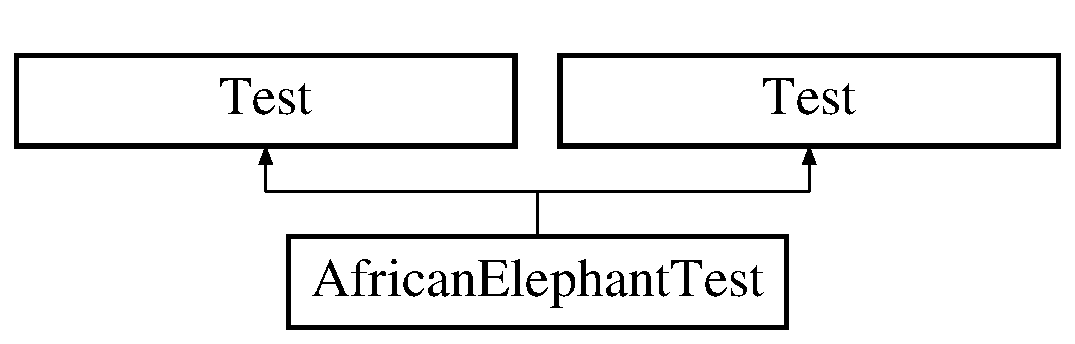
\includegraphics[height=2.000000cm]{class_african_elephant_test}
\end{center}
\end{figure}


The documentation for this class was generated from the following files\+:\begin{DoxyCompactItemize}
\item 
africanelephant\+\_\+test.\+cpp\item 
main\+\_\+test.\+cpp\end{DoxyCompactItemize}

\hypertarget{class_air_habitat}{}\section{Air\+Habitat Class Reference}
\label{class_air_habitat}\index{Air\+Habitat@{Air\+Habitat}}
\subsection*{Public Member Functions}
\begin{DoxyCompactItemize}
\item 
\hyperlink{class_air_habitat_aaf82e1201cb35917975fa58ac5a67763}{Air\+Habitat} ()
\begin{DoxyCompactList}\small\item\em constructor \end{DoxyCompactList}\item 
virtual \hyperlink{class_air_habitat_a18f98f33d3edbb7c397e184f3b7ad56b}{$\sim$\+Air\+Habitat} ()\hypertarget{class_air_habitat_a18f98f33d3edbb7c397e184f3b7ad56b}{}\label{class_air_habitat_a18f98f33d3edbb7c397e184f3b7ad56b}

\begin{DoxyCompactList}\small\item\em Destructor. \end{DoxyCompactList}\item 
char \hyperlink{class_air_habitat_a58342f9774797af46bf8f86695568180}{Get\+Render} ()
\begin{DoxyCompactList}\small\item\em render nawn \end{DoxyCompactList}\end{DoxyCompactItemize}


\subsection{Constructor \& Destructor Documentation}
\index{Air\+Habitat@{Air\+Habitat}!Air\+Habitat@{Air\+Habitat}}
\index{Air\+Habitat@{Air\+Habitat}!Air\+Habitat@{Air\+Habitat}}
\subsubsection[{\texorpdfstring{Air\+Habitat()}{AirHabitat()}}]{\setlength{\rightskip}{0pt plus 5cm}Air\+Habitat\+::\+Air\+Habitat (
\begin{DoxyParamCaption}
{}
\end{DoxyParamCaption}
)}\hypertarget{class_air_habitat_aaf82e1201cb35917975fa58ac5a67763}{}\label{class_air_habitat_aaf82e1201cb35917975fa58ac5a67763}


constructor 


\begin{DoxyParams}{Parameters}
{\em posx} & posisi x \\
\hline
{\em posy} & posisi y \\
\hline
\end{DoxyParams}


\subsection{Member Function Documentation}
\index{Air\+Habitat@{Air\+Habitat}!Get\+Render@{Get\+Render}}
\index{Get\+Render@{Get\+Render}!Air\+Habitat@{Air\+Habitat}}
\subsubsection[{\texorpdfstring{Get\+Render()}{GetRender()}}]{\setlength{\rightskip}{0pt plus 5cm}char Air\+Habitat\+::\+Get\+Render (
\begin{DoxyParamCaption}
{}
\end{DoxyParamCaption}
)}\hypertarget{class_air_habitat_a58342f9774797af46bf8f86695568180}{}\label{class_air_habitat_a58342f9774797af46bf8f86695568180}


render nawn 


\begin{DoxyParams}{Parameters}
{\em cc} & nawnnawn \\
\hline
\end{DoxyParams}


The documentation for this class was generated from the following files\+:\begin{DoxyCompactItemize}
\item 
air\+\_\+habitat.\+h\item 
air\+\_\+habitat.\+cpp\end{DoxyCompactItemize}

\hypertarget{class_air_habitat_test}{}\section{Air\+Habitat\+Test Class Reference}
\label{class_air_habitat_test}\index{Air\+Habitat\+Test@{Air\+Habitat\+Test}}
Inheritance diagram for Air\+Habitat\+Test\+:\begin{figure}[H]
\begin{center}
\leavevmode
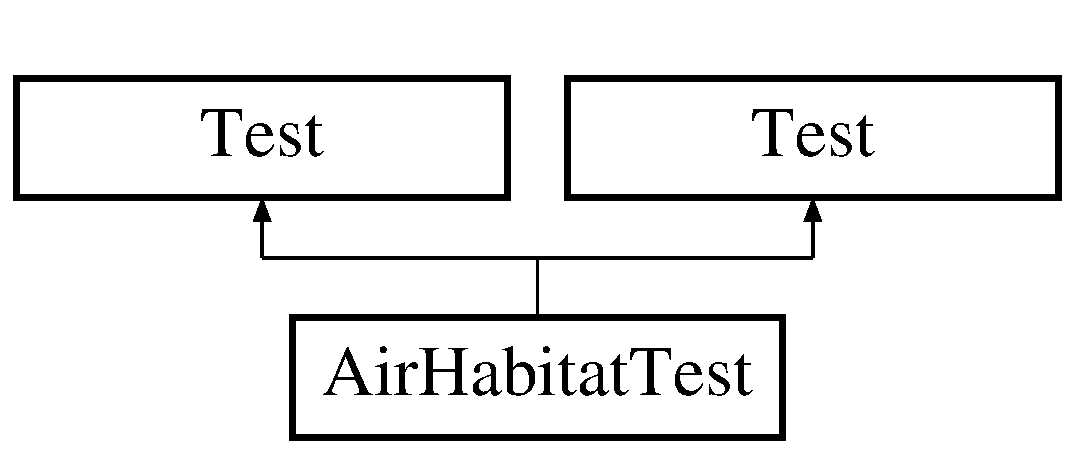
\includegraphics[height=2.000000cm]{class_air_habitat_test}
\end{center}
\end{figure}


The documentation for this class was generated from the following files\+:\begin{DoxyCompactItemize}
\item 
air\+\_\+habitat\+\_\+test.\+cpp\item 
main\+\_\+test.\+cpp\end{DoxyCompactItemize}

\hypertarget{class_anoa}{}\section{Anoa Class Reference}
\label{class_anoa}\index{Anoa@{Anoa}}
\subsection*{Public Member Functions}
\begin{DoxyCompactItemize}
\item 
\hyperlink{class_anoa_adc03b4c166e61ef3c66c84bb9f74d037}{Anoa} ()\hypertarget{class_anoa_adc03b4c166e61ef3c66c84bb9f74d037}{}\label{class_anoa_adc03b4c166e61ef3c66c84bb9f74d037}

\begin{DoxyCompactList}\small\item\em Inisialisasi Hewan. \end{DoxyCompactList}\item 
\hyperlink{class_anoa_ab80d0e5f30d7b6a008e56f4fad144ecf}{$\sim$\+Anoa} ()\hypertarget{class_anoa_ab80d0e5f30d7b6a008e56f4fad144ecf}{}\label{class_anoa_ab80d0e5f30d7b6a008e56f4fad144ecf}

\begin{DoxyCompactList}\small\item\em Destructor. \end{DoxyCompactList}\item 
string \hyperlink{class_anoa_a5873ad7fbbaabe159fe78d18abca5cf9}{Get\+Experience} ()\hypertarget{class_anoa_a5873ad7fbbaabe159fe78d18abca5cf9}{}\label{class_anoa_a5873ad7fbbaabe159fe78d18abca5cf9}

\begin{DoxyCompactList}\small\item\em Komunikasi dengan hewan. \end{DoxyCompactList}\item 
int \hyperlink{class_anoa_a1bd6ef587f919996a80664ce7fe378f4}{Get\+Food\+Num} ()
\begin{DoxyCompactList}\small\item\em Jumlah makanan. \end{DoxyCompactList}\item 
char \hyperlink{class_anoa_aa18da9e26b96be2ab14510cab0753653}{Get\+Render} ()
\begin{DoxyCompactList}\small\item\em Print karakter. \end{DoxyCompactList}\item 
void \hyperlink{class_anoa_a3e2a743b367371207a4f511542016c9f}{Set\+Enemy} (char cc)
\begin{DoxyCompactList}\small\item\em Set karakter hewan. \end{DoxyCompactList}\item 
char $\ast$ \hyperlink{class_anoa_aebfc13ce0edf718e7ad691ce227444dc}{Get\+Enemy} ()
\begin{DoxyCompactList}\small\item\em Ambil list musuh. \end{DoxyCompactList}\end{DoxyCompactItemize}
\subsection*{Protected Attributes}
\begin{DoxyCompactItemize}
\item 
int $\ast$ \hyperlink{class_anoa_a074ddc510aa6b04d78100f1d9d562f2e}{Type}
\item 
string \hyperlink{class_anoa_a70b854fa12421457338081ff66e23b3c}{Famili}
\item 
string \hyperlink{class_anoa_a6dffd5df83dbf71071233b6c32aac878}{Species}
\item 
string \hyperlink{class_anoa_a6791e3fbe425ec1b478dcf2544c039aa}{Experience}
\item 
short \hyperlink{class_anoa_af710bb7dedfd5ea717db3c940981d3e9}{Jenis\+Makanan}
\item 
int \hyperlink{class_anoa_ace1d7758a5e8371a22b23fecbf9152e7}{Berat}
\item 
char \hyperlink{class_anoa_a4bfb9cb19e5c6c784d8e60b060f7fa7f}{Ani\+Char}
\item 
char $\ast$ \hyperlink{class_anoa_abc7657c0df0c0a08b69c9fd9213442f2}{Enemy\+Char}
\item 
int \hyperlink{class_anoa_ae36a4e73eaeed7952baf5804ea68cdc2}{Top\+Enemy}
\end{DoxyCompactItemize}


\subsection{Member Function Documentation}
\index{Anoa@{Anoa}!Get\+Enemy@{Get\+Enemy}}
\index{Get\+Enemy@{Get\+Enemy}!Anoa@{Anoa}}
\subsubsection[{\texorpdfstring{Get\+Enemy()}{GetEnemy()}}]{\setlength{\rightskip}{0pt plus 5cm}char $\ast$ Anoa\+::\+Get\+Enemy (
\begin{DoxyParamCaption}
{}
\end{DoxyParamCaption}
)}\hypertarget{class_anoa_aebfc13ce0edf718e7ad691ce227444dc}{}\label{class_anoa_aebfc13ce0edf718e7ad691ce227444dc}


Ambil list musuh. 

\begin{DoxyReturn}{Returns}
List Musuh 
\end{DoxyReturn}
\index{Anoa@{Anoa}!Get\+Food\+Num@{Get\+Food\+Num}}
\index{Get\+Food\+Num@{Get\+Food\+Num}!Anoa@{Anoa}}
\subsubsection[{\texorpdfstring{Get\+Food\+Num()}{GetFoodNum()}}]{\setlength{\rightskip}{0pt plus 5cm}int Anoa\+::\+Get\+Food\+Num (
\begin{DoxyParamCaption}
{}
\end{DoxyParamCaption}
)}\hypertarget{class_anoa_a1bd6ef587f919996a80664ce7fe378f4}{}\label{class_anoa_a1bd6ef587f919996a80664ce7fe378f4}


Jumlah makanan. 

\begin{DoxyReturn}{Returns}
Jumlah makan

Jumlah makanan 
\end{DoxyReturn}
\index{Anoa@{Anoa}!Get\+Render@{Get\+Render}}
\index{Get\+Render@{Get\+Render}!Anoa@{Anoa}}
\subsubsection[{\texorpdfstring{Get\+Render()}{GetRender()}}]{\setlength{\rightskip}{0pt plus 5cm}char Anoa\+::\+Get\+Render (
\begin{DoxyParamCaption}
{}
\end{DoxyParamCaption}
)}\hypertarget{class_anoa_aa18da9e26b96be2ab14510cab0753653}{}\label{class_anoa_aa18da9e26b96be2ab14510cab0753653}


Print karakter. 

\begin{DoxyReturn}{Returns}
char 
\end{DoxyReturn}
\index{Anoa@{Anoa}!Set\+Enemy@{Set\+Enemy}}
\index{Set\+Enemy@{Set\+Enemy}!Anoa@{Anoa}}
\subsubsection[{\texorpdfstring{Set\+Enemy(char cc)}{SetEnemy(char cc)}}]{\setlength{\rightskip}{0pt plus 5cm}void Anoa\+::\+Set\+Enemy (
\begin{DoxyParamCaption}
\item[{char}]{cc}
\end{DoxyParamCaption}
)}\hypertarget{class_anoa_a3e2a743b367371207a4f511542016c9f}{}\label{class_anoa_a3e2a743b367371207a4f511542016c9f}


Set karakter hewan. 


\begin{DoxyParams}{Parameters}
{\em cc} & Karakter hewan tsb \\
\hline
\end{DoxyParams}


\subsection{Member Data Documentation}
\index{Anoa@{Anoa}!Ani\+Char@{Ani\+Char}}
\index{Ani\+Char@{Ani\+Char}!Anoa@{Anoa}}
\subsubsection[{\texorpdfstring{Ani\+Char}{AniChar}}]{\setlength{\rightskip}{0pt plus 5cm}char Anoa\+::\+Ani\+Char\hspace{0.3cm}{\ttfamily [protected]}}\hypertarget{class_anoa_a4bfb9cb19e5c6c784d8e60b060f7fa7f}{}\label{class_anoa_a4bfb9cb19e5c6c784d8e60b060f7fa7f}
Char yang digunakan untuk render \index{Anoa@{Anoa}!Berat@{Berat}}
\index{Berat@{Berat}!Anoa@{Anoa}}
\subsubsection[{\texorpdfstring{Berat}{Berat}}]{\setlength{\rightskip}{0pt plus 5cm}int Anoa\+::\+Berat\hspace{0.3cm}{\ttfamily [protected]}}\hypertarget{class_anoa_ace1d7758a5e8371a22b23fecbf9152e7}{}\label{class_anoa_ace1d7758a5e8371a22b23fecbf9152e7}
Berat hewan \index{Anoa@{Anoa}!Enemy\+Char@{Enemy\+Char}}
\index{Enemy\+Char@{Enemy\+Char}!Anoa@{Anoa}}
\subsubsection[{\texorpdfstring{Enemy\+Char}{EnemyChar}}]{\setlength{\rightskip}{0pt plus 5cm}char$\ast$ Anoa\+::\+Enemy\+Char\hspace{0.3cm}{\ttfamily [protected]}}\hypertarget{class_anoa_abc7657c0df0c0a08b69c9fd9213442f2}{}\label{class_anoa_abc7657c0df0c0a08b69c9fd9213442f2}
Array of char yang berisi list musuhnya \index{Anoa@{Anoa}!Experience@{Experience}}
\index{Experience@{Experience}!Anoa@{Anoa}}
\subsubsection[{\texorpdfstring{Experience}{Experience}}]{\setlength{\rightskip}{0pt plus 5cm}string Anoa\+::\+Experience\hspace{0.3cm}{\ttfamily [protected]}}\hypertarget{class_anoa_a6791e3fbe425ec1b478dcf2544c039aa}{}\label{class_anoa_a6791e3fbe425ec1b478dcf2544c039aa}
Experience hewan \index{Anoa@{Anoa}!Famili@{Famili}}
\index{Famili@{Famili}!Anoa@{Anoa}}
\subsubsection[{\texorpdfstring{Famili}{Famili}}]{\setlength{\rightskip}{0pt plus 5cm}string Anoa\+::\+Famili\hspace{0.3cm}{\ttfamily [protected]}}\hypertarget{class_anoa_a70b854fa12421457338081ff66e23b3c}{}\label{class_anoa_a70b854fa12421457338081ff66e23b3c}
Family hewan \index{Anoa@{Anoa}!Jenis\+Makanan@{Jenis\+Makanan}}
\index{Jenis\+Makanan@{Jenis\+Makanan}!Anoa@{Anoa}}
\subsubsection[{\texorpdfstring{Jenis\+Makanan}{JenisMakanan}}]{\setlength{\rightskip}{0pt plus 5cm}short Anoa\+::\+Jenis\+Makanan\hspace{0.3cm}{\ttfamily [protected]}}\hypertarget{class_anoa_af710bb7dedfd5ea717db3c940981d3e9}{}\label{class_anoa_af710bb7dedfd5ea717db3c940981d3e9}
Jenis Makanan hewan. 1 \+: herbifor, 2 \+: karnivor, 3 \+: omnifor \index{Anoa@{Anoa}!Species@{Species}}
\index{Species@{Species}!Anoa@{Anoa}}
\subsubsection[{\texorpdfstring{Species}{Species}}]{\setlength{\rightskip}{0pt plus 5cm}string Anoa\+::\+Species\hspace{0.3cm}{\ttfamily [protected]}}\hypertarget{class_anoa_a6dffd5df83dbf71071233b6c32aac878}{}\label{class_anoa_a6dffd5df83dbf71071233b6c32aac878}
Species hewan \index{Anoa@{Anoa}!Top\+Enemy@{Top\+Enemy}}
\index{Top\+Enemy@{Top\+Enemy}!Anoa@{Anoa}}
\subsubsection[{\texorpdfstring{Top\+Enemy}{TopEnemy}}]{\setlength{\rightskip}{0pt plus 5cm}int Anoa\+::\+Top\+Enemy\hspace{0.3cm}{\ttfamily [protected]}}\hypertarget{class_anoa_ae36a4e73eaeed7952baf5804ea68cdc2}{}\label{class_anoa_ae36a4e73eaeed7952baf5804ea68cdc2}
Pointer Enemy\+Char yang available \index{Anoa@{Anoa}!Type@{Type}}
\index{Type@{Type}!Anoa@{Anoa}}
\subsubsection[{\texorpdfstring{Type}{Type}}]{\setlength{\rightskip}{0pt plus 5cm}int$\ast$ Anoa\+::\+Type\hspace{0.3cm}{\ttfamily [protected]}}\hypertarget{class_anoa_a074ddc510aa6b04d78100f1d9d562f2e}{}\label{class_anoa_a074ddc510aa6b04d78100f1d9d562f2e}
Type habitat hewan. 0 \+: darat, 1 \+: udara, 2 \+: air 

The documentation for this class was generated from the following files\+:\begin{DoxyCompactItemize}
\item 
anoa.\+h\item 
anoa.\+cpp\end{DoxyCompactItemize}

\hypertarget{class_anoa_test}{}\section{Anoa\+Test Class Reference}
\label{class_anoa_test}\index{Anoa\+Test@{Anoa\+Test}}
Inheritance diagram for Anoa\+Test\+:\begin{figure}[H]
\begin{center}
\leavevmode
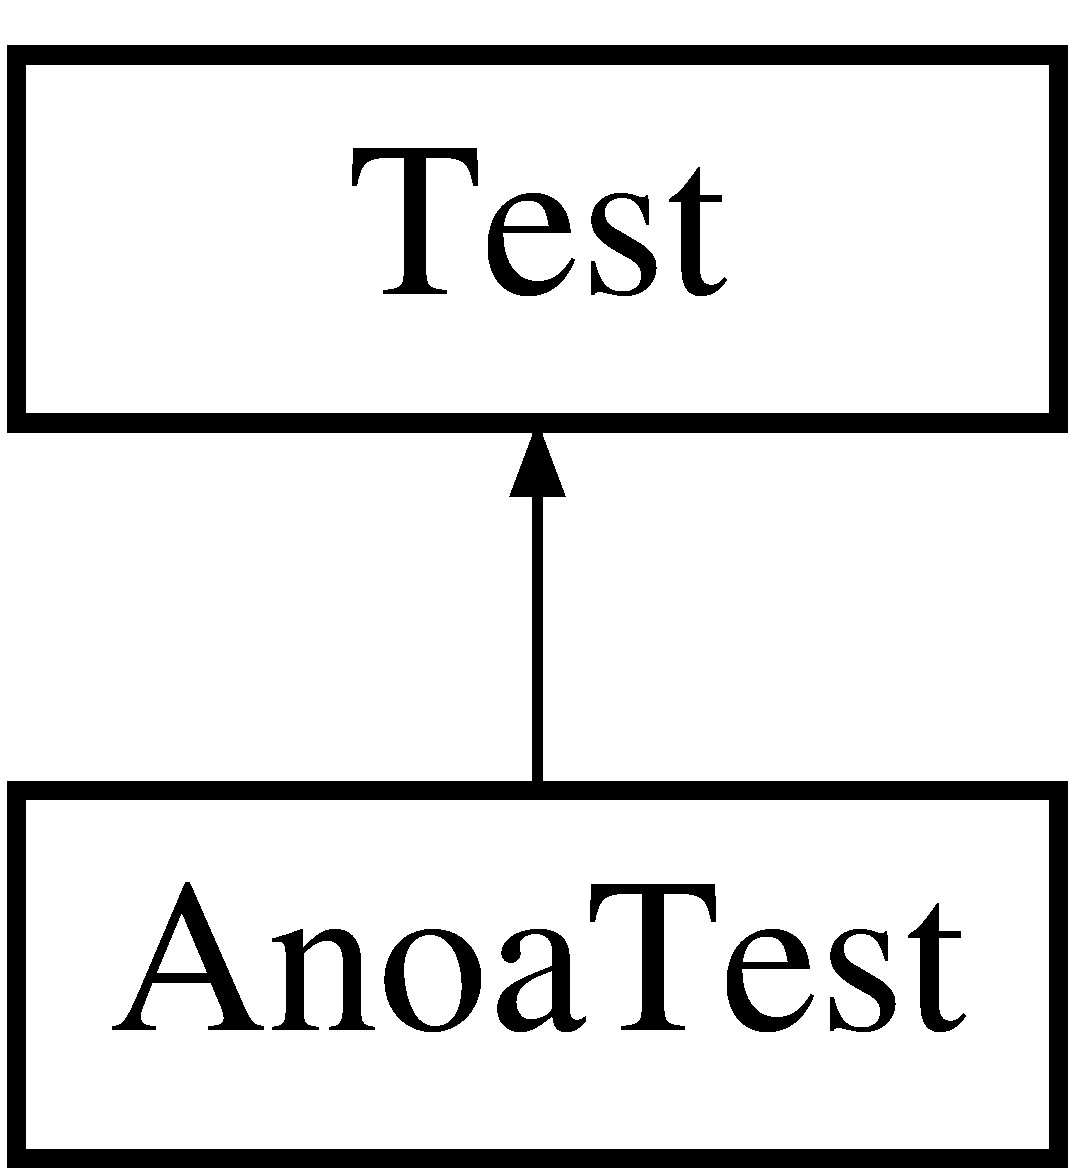
\includegraphics[height=2.000000cm]{class_anoa_test}
\end{center}
\end{figure}


The documentation for this class was generated from the following file\+:\begin{DoxyCompactItemize}
\item 
main\+\_\+test.\+cpp\end{DoxyCompactItemize}

\hypertarget{class_bear}{}\section{Bear Class Reference}
\label{class_bear}\index{Bear@{Bear}}
\subsection*{Public Member Functions}
\begin{DoxyCompactItemize}
\item 
\hyperlink{class_bear_a639d2d41ec84454055f7b44f23c39639}{Bear} ()\hypertarget{class_bear_a639d2d41ec84454055f7b44f23c39639}{}\label{class_bear_a639d2d41ec84454055f7b44f23c39639}

\begin{DoxyCompactList}\small\item\em Inisialisasi Hewan. \end{DoxyCompactList}\item 
\hyperlink{class_bear_aa76f45b1665a93512b04af11a0346b4f}{$\sim$\+Bear} ()\hypertarget{class_bear_aa76f45b1665a93512b04af11a0346b4f}{}\label{class_bear_aa76f45b1665a93512b04af11a0346b4f}

\begin{DoxyCompactList}\small\item\em Destructor. \end{DoxyCompactList}\item 
string \hyperlink{class_bear_a2df1a07339534654f35de034ea3dafcb}{Get\+Experience} ()\hypertarget{class_bear_a2df1a07339534654f35de034ea3dafcb}{}\label{class_bear_a2df1a07339534654f35de034ea3dafcb}

\begin{DoxyCompactList}\small\item\em Komunikasi dengan hewan. \end{DoxyCompactList}\item 
int \hyperlink{class_bear_a4b57abf5bb55df3b222af850f5d033d7}{Get\+Food\+Num} ()
\begin{DoxyCompactList}\small\item\em Jumlah makanan. \end{DoxyCompactList}\item 
char \hyperlink{class_bear_a2d653d61990d3d72393ceaee126347d6}{Get\+Render} ()
\begin{DoxyCompactList}\small\item\em Print karakter. \end{DoxyCompactList}\item 
void \hyperlink{class_bear_a7506c9aca8c458184e92b51747602799}{Set\+Enemy} (char cc)
\begin{DoxyCompactList}\small\item\em Set karakter hewan. \end{DoxyCompactList}\item 
char $\ast$ \hyperlink{class_bear_aacb1d0bd094175bdb2105f22c5639e13}{Get\+Enemy} ()
\begin{DoxyCompactList}\small\item\em Ambil list musuh. \end{DoxyCompactList}\end{DoxyCompactItemize}
\subsection*{Protected Attributes}
\begin{DoxyCompactItemize}
\item 
int $\ast$ \hyperlink{class_bear_a03e9a8157b73c13012c774d1cc2dc2ce}{Type}
\item 
string \hyperlink{class_bear_a767087abd9a85df8d7d491468a38c31c}{Famili}
\item 
string \hyperlink{class_bear_a2fb3468c903430fc04e61d746fdc0ca4}{Species}
\item 
string \hyperlink{class_bear_af37839ada6bce88bfa2eecc5594a14f3}{Experience}
\item 
short \hyperlink{class_bear_af7d119e505bc59bdf0dc57798a513411}{Jenis\+Makanan}
\item 
int \hyperlink{class_bear_ae3d0faff07047afc333f43cdd4633afd}{Berat}
\item 
char \hyperlink{class_bear_a9745d3b799240db3554f6da9708d5cdd}{Ani\+Char}
\item 
char $\ast$ \hyperlink{class_bear_a035b584369de54e3d25d7e19aa99ee6d}{Enemy\+Char}
\item 
int \hyperlink{class_bear_a7d03f6795109ce70a28a7941394868a1}{Top\+Enemy}
\end{DoxyCompactItemize}


\subsection{Member Function Documentation}
\index{Bear@{Bear}!Get\+Enemy@{Get\+Enemy}}
\index{Get\+Enemy@{Get\+Enemy}!Bear@{Bear}}
\subsubsection[{\texorpdfstring{Get\+Enemy()}{GetEnemy()}}]{\setlength{\rightskip}{0pt plus 5cm}char $\ast$ Bear\+::\+Get\+Enemy (
\begin{DoxyParamCaption}
{}
\end{DoxyParamCaption}
)}\hypertarget{class_bear_aacb1d0bd094175bdb2105f22c5639e13}{}\label{class_bear_aacb1d0bd094175bdb2105f22c5639e13}


Ambil list musuh. 

\begin{DoxyReturn}{Returns}
List Musuh 
\end{DoxyReturn}
\index{Bear@{Bear}!Get\+Food\+Num@{Get\+Food\+Num}}
\index{Get\+Food\+Num@{Get\+Food\+Num}!Bear@{Bear}}
\subsubsection[{\texorpdfstring{Get\+Food\+Num()}{GetFoodNum()}}]{\setlength{\rightskip}{0pt plus 5cm}int Bear\+::\+Get\+Food\+Num (
\begin{DoxyParamCaption}
{}
\end{DoxyParamCaption}
)}\hypertarget{class_bear_a4b57abf5bb55df3b222af850f5d033d7}{}\label{class_bear_a4b57abf5bb55df3b222af850f5d033d7}


Jumlah makanan. 

\begin{DoxyReturn}{Returns}
Jumlah makan

Jumlah makanan 
\end{DoxyReturn}
\index{Bear@{Bear}!Get\+Render@{Get\+Render}}
\index{Get\+Render@{Get\+Render}!Bear@{Bear}}
\subsubsection[{\texorpdfstring{Get\+Render()}{GetRender()}}]{\setlength{\rightskip}{0pt plus 5cm}char Bear\+::\+Get\+Render (
\begin{DoxyParamCaption}
{}
\end{DoxyParamCaption}
)}\hypertarget{class_bear_a2d653d61990d3d72393ceaee126347d6}{}\label{class_bear_a2d653d61990d3d72393ceaee126347d6}


Print karakter. 

\begin{DoxyReturn}{Returns}
char 
\end{DoxyReturn}
\index{Bear@{Bear}!Set\+Enemy@{Set\+Enemy}}
\index{Set\+Enemy@{Set\+Enemy}!Bear@{Bear}}
\subsubsection[{\texorpdfstring{Set\+Enemy(char cc)}{SetEnemy(char cc)}}]{\setlength{\rightskip}{0pt plus 5cm}void Bear\+::\+Set\+Enemy (
\begin{DoxyParamCaption}
\item[{char}]{cc}
\end{DoxyParamCaption}
)}\hypertarget{class_bear_a7506c9aca8c458184e92b51747602799}{}\label{class_bear_a7506c9aca8c458184e92b51747602799}


Set karakter hewan. 


\begin{DoxyParams}{Parameters}
{\em cc} & Karakter hewan tsb \\
\hline
\end{DoxyParams}


\subsection{Member Data Documentation}
\index{Bear@{Bear}!Ani\+Char@{Ani\+Char}}
\index{Ani\+Char@{Ani\+Char}!Bear@{Bear}}
\subsubsection[{\texorpdfstring{Ani\+Char}{AniChar}}]{\setlength{\rightskip}{0pt plus 5cm}char Bear\+::\+Ani\+Char\hspace{0.3cm}{\ttfamily [protected]}}\hypertarget{class_bear_a9745d3b799240db3554f6da9708d5cdd}{}\label{class_bear_a9745d3b799240db3554f6da9708d5cdd}
Char yang digunakan untuk render \index{Bear@{Bear}!Berat@{Berat}}
\index{Berat@{Berat}!Bear@{Bear}}
\subsubsection[{\texorpdfstring{Berat}{Berat}}]{\setlength{\rightskip}{0pt plus 5cm}int Bear\+::\+Berat\hspace{0.3cm}{\ttfamily [protected]}}\hypertarget{class_bear_ae3d0faff07047afc333f43cdd4633afd}{}\label{class_bear_ae3d0faff07047afc333f43cdd4633afd}
Berat hewan \index{Bear@{Bear}!Enemy\+Char@{Enemy\+Char}}
\index{Enemy\+Char@{Enemy\+Char}!Bear@{Bear}}
\subsubsection[{\texorpdfstring{Enemy\+Char}{EnemyChar}}]{\setlength{\rightskip}{0pt plus 5cm}char$\ast$ Bear\+::\+Enemy\+Char\hspace{0.3cm}{\ttfamily [protected]}}\hypertarget{class_bear_a035b584369de54e3d25d7e19aa99ee6d}{}\label{class_bear_a035b584369de54e3d25d7e19aa99ee6d}
Array of char yang berisi list musuhnya \index{Bear@{Bear}!Experience@{Experience}}
\index{Experience@{Experience}!Bear@{Bear}}
\subsubsection[{\texorpdfstring{Experience}{Experience}}]{\setlength{\rightskip}{0pt plus 5cm}string Bear\+::\+Experience\hspace{0.3cm}{\ttfamily [protected]}}\hypertarget{class_bear_af37839ada6bce88bfa2eecc5594a14f3}{}\label{class_bear_af37839ada6bce88bfa2eecc5594a14f3}
Experience hewan \index{Bear@{Bear}!Famili@{Famili}}
\index{Famili@{Famili}!Bear@{Bear}}
\subsubsection[{\texorpdfstring{Famili}{Famili}}]{\setlength{\rightskip}{0pt plus 5cm}string Bear\+::\+Famili\hspace{0.3cm}{\ttfamily [protected]}}\hypertarget{class_bear_a767087abd9a85df8d7d491468a38c31c}{}\label{class_bear_a767087abd9a85df8d7d491468a38c31c}
Family hewan \index{Bear@{Bear}!Jenis\+Makanan@{Jenis\+Makanan}}
\index{Jenis\+Makanan@{Jenis\+Makanan}!Bear@{Bear}}
\subsubsection[{\texorpdfstring{Jenis\+Makanan}{JenisMakanan}}]{\setlength{\rightskip}{0pt plus 5cm}short Bear\+::\+Jenis\+Makanan\hspace{0.3cm}{\ttfamily [protected]}}\hypertarget{class_bear_af7d119e505bc59bdf0dc57798a513411}{}\label{class_bear_af7d119e505bc59bdf0dc57798a513411}
Jenis Makanan hewan. 1 \+: herbifor, 2 \+: karnivor, 3 \+: omnifor \index{Bear@{Bear}!Species@{Species}}
\index{Species@{Species}!Bear@{Bear}}
\subsubsection[{\texorpdfstring{Species}{Species}}]{\setlength{\rightskip}{0pt plus 5cm}string Bear\+::\+Species\hspace{0.3cm}{\ttfamily [protected]}}\hypertarget{class_bear_a2fb3468c903430fc04e61d746fdc0ca4}{}\label{class_bear_a2fb3468c903430fc04e61d746fdc0ca4}
Species hewan \index{Bear@{Bear}!Top\+Enemy@{Top\+Enemy}}
\index{Top\+Enemy@{Top\+Enemy}!Bear@{Bear}}
\subsubsection[{\texorpdfstring{Top\+Enemy}{TopEnemy}}]{\setlength{\rightskip}{0pt plus 5cm}int Bear\+::\+Top\+Enemy\hspace{0.3cm}{\ttfamily [protected]}}\hypertarget{class_bear_a7d03f6795109ce70a28a7941394868a1}{}\label{class_bear_a7d03f6795109ce70a28a7941394868a1}
Pointer Enemy\+Char yang available \index{Bear@{Bear}!Type@{Type}}
\index{Type@{Type}!Bear@{Bear}}
\subsubsection[{\texorpdfstring{Type}{Type}}]{\setlength{\rightskip}{0pt plus 5cm}int$\ast$ Bear\+::\+Type\hspace{0.3cm}{\ttfamily [protected]}}\hypertarget{class_bear_a03e9a8157b73c13012c774d1cc2dc2ce}{}\label{class_bear_a03e9a8157b73c13012c774d1cc2dc2ce}
Type habitat hewan. 0 \+: darat, 1 \+: udara, 2 \+: air 

The documentation for this class was generated from the following files\+:\begin{DoxyCompactItemize}
\item 
bear.\+h\item 
bear.\+cpp\end{DoxyCompactItemize}

\hypertarget{class_bear_test}{}\section{Bear\+Test Class Reference}
\label{class_bear_test}\index{Bear\+Test@{Bear\+Test}}
Inheritance diagram for Bear\+Test\+:\begin{figure}[H]
\begin{center}
\leavevmode
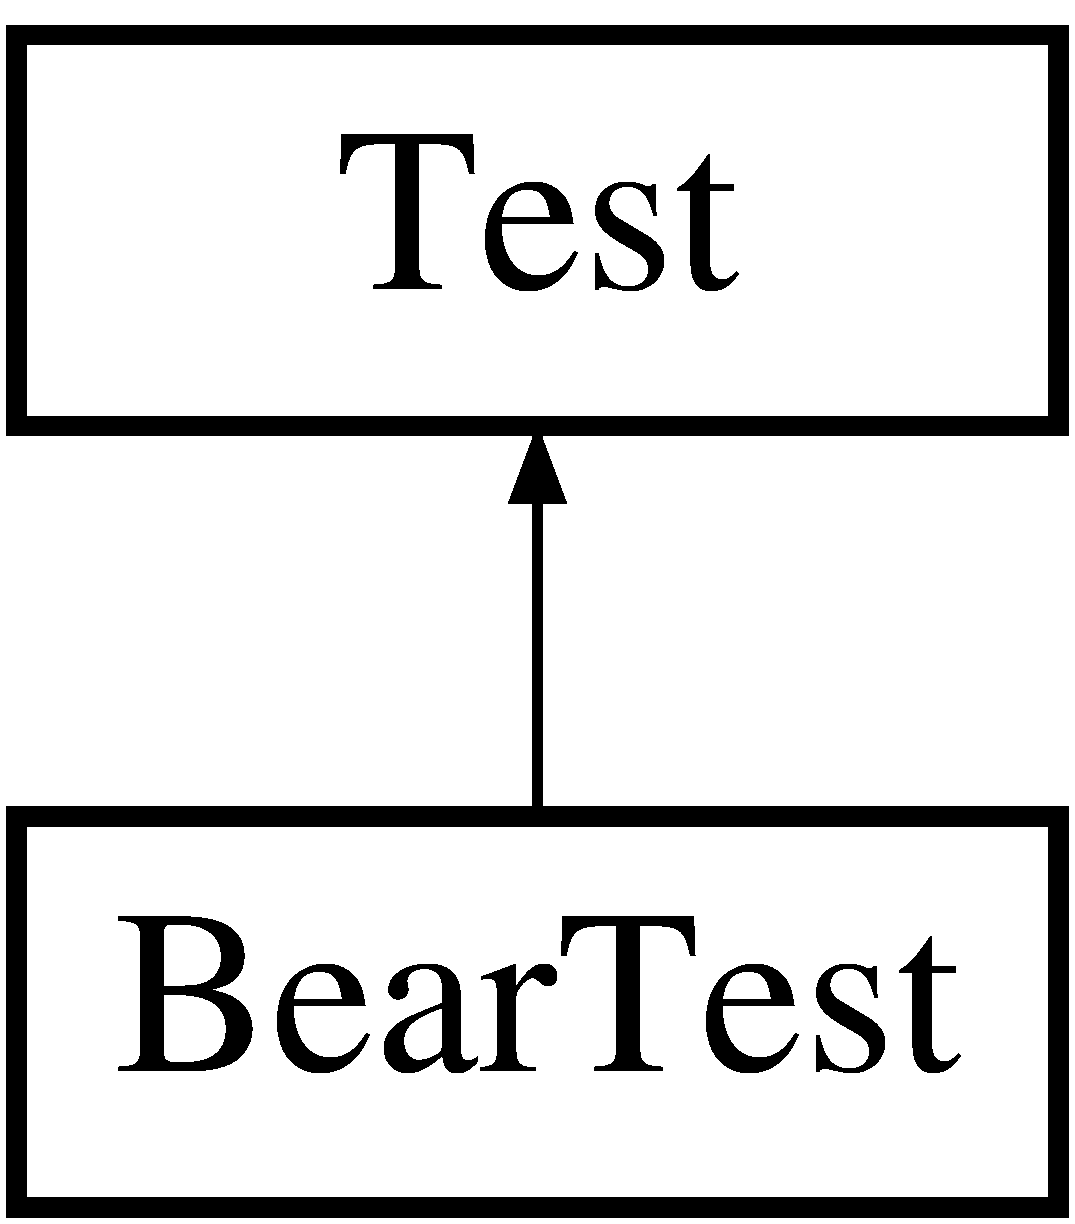
\includegraphics[height=2.000000cm]{class_bear_test}
\end{center}
\end{figure}


The documentation for this class was generated from the following file\+:\begin{DoxyCompactItemize}
\item 
main\+\_\+test.\+cpp\end{DoxyCompactItemize}

\hypertarget{class_eagle}{}\section{Eagle Class Reference}
\label{class_eagle}\index{Eagle@{Eagle}}
\subsection*{Public Member Functions}
\begin{DoxyCompactItemize}
\item 
\hyperlink{class_eagle_a8b205e5b26bece07d18b852b042851fe}{Eagle} ()\hypertarget{class_eagle_a8b205e5b26bece07d18b852b042851fe}{}\label{class_eagle_a8b205e5b26bece07d18b852b042851fe}

\begin{DoxyCompactList}\small\item\em Constructor. \end{DoxyCompactList}\item 
\hyperlink{class_eagle_a192a898182736506c1f78159bf3477b7}{$\sim$\+Eagle} ()\hypertarget{class_eagle_a192a898182736506c1f78159bf3477b7}{}\label{class_eagle_a192a898182736506c1f78159bf3477b7}

\begin{DoxyCompactList}\small\item\em Destructor. \end{DoxyCompactList}\item 
string \hyperlink{class_eagle_abba7200880762e44c4d4efd022b4fdf5}{Get\+Experience} ()\hypertarget{class_eagle_abba7200880762e44c4d4efd022b4fdf5}{}\label{class_eagle_abba7200880762e44c4d4efd022b4fdf5}

\begin{DoxyCompactList}\small\item\em Komunikasi dengan hewan. \end{DoxyCompactList}\item 
int \hyperlink{class_eagle_a17c7f9dee204950dbdfae50b9ac3b109}{Get\+Food\+Num} ()
\begin{DoxyCompactList}\small\item\em Jumlah makanan. \end{DoxyCompactList}\item 
char \hyperlink{class_eagle_a3c1666b9eb07da8a1f45a230f72c7e14}{Get\+Render} ()
\begin{DoxyCompactList}\small\item\em Print karakter. \end{DoxyCompactList}\item 
void \hyperlink{class_eagle_ac6aec7ed7fe21d00009ef2fdfa89e906}{Set\+Enemy} (char cc)
\begin{DoxyCompactList}\small\item\em Set karakter hewan. \end{DoxyCompactList}\item 
char $\ast$ \hyperlink{class_eagle_ae236ae54ae034fe9a28c16b5da250351}{Get\+Enemy} ()
\begin{DoxyCompactList}\small\item\em Ambil list musuh. \end{DoxyCompactList}\end{DoxyCompactItemize}
\subsection*{Protected Attributes}
\begin{DoxyCompactItemize}
\item 
int $\ast$ \hyperlink{class_eagle_a95800352867fbd31040582cc79c18b82}{Type}
\item 
string \hyperlink{class_eagle_ade0d4181358630d065569538501f6132}{Famili}
\item 
string \hyperlink{class_eagle_a61f705b57074941915461034802176f2}{Species}
\item 
string \hyperlink{class_eagle_aa0cc19789f81ee5816af9bdcdb317c95}{Experience}
\item 
short \hyperlink{class_eagle_a55a9be317085d72e732d3ce8f30d5ba3}{Jenis\+Makanan}
\item 
int \hyperlink{class_eagle_ad67052387c7a14e70884eb64543371e6}{Berat}
\item 
char \hyperlink{class_eagle_a51848217dd4b104fde6fdcfc56b747b8}{Ani\+Char}
\item 
char $\ast$ \hyperlink{class_eagle_aa022a6488691235bca90587719675ebc}{Enemy\+Char}
\item 
int \hyperlink{class_eagle_a5b4809208017e8864727510d26436a0b}{Top\+Enemy}
\end{DoxyCompactItemize}


\subsection{Member Function Documentation}
\index{Eagle@{Eagle}!Get\+Enemy@{Get\+Enemy}}
\index{Get\+Enemy@{Get\+Enemy}!Eagle@{Eagle}}
\subsubsection[{\texorpdfstring{Get\+Enemy()}{GetEnemy()}}]{\setlength{\rightskip}{0pt plus 5cm}char $\ast$ Eagle\+::\+Get\+Enemy (
\begin{DoxyParamCaption}
{}
\end{DoxyParamCaption}
)}\hypertarget{class_eagle_ae236ae54ae034fe9a28c16b5da250351}{}\label{class_eagle_ae236ae54ae034fe9a28c16b5da250351}


Ambil list musuh. 

\begin{DoxyReturn}{Returns}
List Musuh 
\end{DoxyReturn}
\index{Eagle@{Eagle}!Get\+Food\+Num@{Get\+Food\+Num}}
\index{Get\+Food\+Num@{Get\+Food\+Num}!Eagle@{Eagle}}
\subsubsection[{\texorpdfstring{Get\+Food\+Num()}{GetFoodNum()}}]{\setlength{\rightskip}{0pt plus 5cm}int Eagle\+::\+Get\+Food\+Num (
\begin{DoxyParamCaption}
{}
\end{DoxyParamCaption}
)}\hypertarget{class_eagle_a17c7f9dee204950dbdfae50b9ac3b109}{}\label{class_eagle_a17c7f9dee204950dbdfae50b9ac3b109}


Jumlah makanan. 

\begin{DoxyReturn}{Returns}
Jumlah makan

Jumlah makanan 
\end{DoxyReturn}
\index{Eagle@{Eagle}!Get\+Render@{Get\+Render}}
\index{Get\+Render@{Get\+Render}!Eagle@{Eagle}}
\subsubsection[{\texorpdfstring{Get\+Render()}{GetRender()}}]{\setlength{\rightskip}{0pt plus 5cm}char Eagle\+::\+Get\+Render (
\begin{DoxyParamCaption}
{}
\end{DoxyParamCaption}
)}\hypertarget{class_eagle_a3c1666b9eb07da8a1f45a230f72c7e14}{}\label{class_eagle_a3c1666b9eb07da8a1f45a230f72c7e14}


Print karakter. 

\begin{DoxyReturn}{Returns}
char 
\end{DoxyReturn}
\index{Eagle@{Eagle}!Set\+Enemy@{Set\+Enemy}}
\index{Set\+Enemy@{Set\+Enemy}!Eagle@{Eagle}}
\subsubsection[{\texorpdfstring{Set\+Enemy(char cc)}{SetEnemy(char cc)}}]{\setlength{\rightskip}{0pt plus 5cm}void Eagle\+::\+Set\+Enemy (
\begin{DoxyParamCaption}
\item[{char}]{cc}
\end{DoxyParamCaption}
)}\hypertarget{class_eagle_ac6aec7ed7fe21d00009ef2fdfa89e906}{}\label{class_eagle_ac6aec7ed7fe21d00009ef2fdfa89e906}


Set karakter hewan. 


\begin{DoxyParams}{Parameters}
{\em cc} & Karakter hewan tsb \\
\hline
\end{DoxyParams}


\subsection{Member Data Documentation}
\index{Eagle@{Eagle}!Ani\+Char@{Ani\+Char}}
\index{Ani\+Char@{Ani\+Char}!Eagle@{Eagle}}
\subsubsection[{\texorpdfstring{Ani\+Char}{AniChar}}]{\setlength{\rightskip}{0pt plus 5cm}char Eagle\+::\+Ani\+Char\hspace{0.3cm}{\ttfamily [protected]}}\hypertarget{class_eagle_a51848217dd4b104fde6fdcfc56b747b8}{}\label{class_eagle_a51848217dd4b104fde6fdcfc56b747b8}
Char yang digunakan untuk render \index{Eagle@{Eagle}!Berat@{Berat}}
\index{Berat@{Berat}!Eagle@{Eagle}}
\subsubsection[{\texorpdfstring{Berat}{Berat}}]{\setlength{\rightskip}{0pt plus 5cm}int Eagle\+::\+Berat\hspace{0.3cm}{\ttfamily [protected]}}\hypertarget{class_eagle_ad67052387c7a14e70884eb64543371e6}{}\label{class_eagle_ad67052387c7a14e70884eb64543371e6}
Berat hewan \index{Eagle@{Eagle}!Enemy\+Char@{Enemy\+Char}}
\index{Enemy\+Char@{Enemy\+Char}!Eagle@{Eagle}}
\subsubsection[{\texorpdfstring{Enemy\+Char}{EnemyChar}}]{\setlength{\rightskip}{0pt plus 5cm}char$\ast$ Eagle\+::\+Enemy\+Char\hspace{0.3cm}{\ttfamily [protected]}}\hypertarget{class_eagle_aa022a6488691235bca90587719675ebc}{}\label{class_eagle_aa022a6488691235bca90587719675ebc}
Array of char yang berisi list musuhnya \index{Eagle@{Eagle}!Experience@{Experience}}
\index{Experience@{Experience}!Eagle@{Eagle}}
\subsubsection[{\texorpdfstring{Experience}{Experience}}]{\setlength{\rightskip}{0pt plus 5cm}string Eagle\+::\+Experience\hspace{0.3cm}{\ttfamily [protected]}}\hypertarget{class_eagle_aa0cc19789f81ee5816af9bdcdb317c95}{}\label{class_eagle_aa0cc19789f81ee5816af9bdcdb317c95}
Experience hewan \index{Eagle@{Eagle}!Famili@{Famili}}
\index{Famili@{Famili}!Eagle@{Eagle}}
\subsubsection[{\texorpdfstring{Famili}{Famili}}]{\setlength{\rightskip}{0pt plus 5cm}string Eagle\+::\+Famili\hspace{0.3cm}{\ttfamily [protected]}}\hypertarget{class_eagle_ade0d4181358630d065569538501f6132}{}\label{class_eagle_ade0d4181358630d065569538501f6132}
Family hewan \index{Eagle@{Eagle}!Jenis\+Makanan@{Jenis\+Makanan}}
\index{Jenis\+Makanan@{Jenis\+Makanan}!Eagle@{Eagle}}
\subsubsection[{\texorpdfstring{Jenis\+Makanan}{JenisMakanan}}]{\setlength{\rightskip}{0pt plus 5cm}short Eagle\+::\+Jenis\+Makanan\hspace{0.3cm}{\ttfamily [protected]}}\hypertarget{class_eagle_a55a9be317085d72e732d3ce8f30d5ba3}{}\label{class_eagle_a55a9be317085d72e732d3ce8f30d5ba3}
Jenis Makanan hewan. 1 \+: herbifor, 2 \+: karnivor, 3 \+: omnifor \index{Eagle@{Eagle}!Species@{Species}}
\index{Species@{Species}!Eagle@{Eagle}}
\subsubsection[{\texorpdfstring{Species}{Species}}]{\setlength{\rightskip}{0pt plus 5cm}string Eagle\+::\+Species\hspace{0.3cm}{\ttfamily [protected]}}\hypertarget{class_eagle_a61f705b57074941915461034802176f2}{}\label{class_eagle_a61f705b57074941915461034802176f2}
Species hewan \index{Eagle@{Eagle}!Top\+Enemy@{Top\+Enemy}}
\index{Top\+Enemy@{Top\+Enemy}!Eagle@{Eagle}}
\subsubsection[{\texorpdfstring{Top\+Enemy}{TopEnemy}}]{\setlength{\rightskip}{0pt plus 5cm}int Eagle\+::\+Top\+Enemy\hspace{0.3cm}{\ttfamily [protected]}}\hypertarget{class_eagle_a5b4809208017e8864727510d26436a0b}{}\label{class_eagle_a5b4809208017e8864727510d26436a0b}
Pointer Enemy\+Char yang available \index{Eagle@{Eagle}!Type@{Type}}
\index{Type@{Type}!Eagle@{Eagle}}
\subsubsection[{\texorpdfstring{Type}{Type}}]{\setlength{\rightskip}{0pt plus 5cm}int$\ast$ Eagle\+::\+Type\hspace{0.3cm}{\ttfamily [protected]}}\hypertarget{class_eagle_a95800352867fbd31040582cc79c18b82}{}\label{class_eagle_a95800352867fbd31040582cc79c18b82}
Type habitat hewan. 0 \+: darat, 1 \+: udara, 2 \+: air 

The documentation for this class was generated from the following files\+:\begin{DoxyCompactItemize}
\item 
eagle.\+h\item 
eagle.\+cpp\end{DoxyCompactItemize}

\hypertarget{class_eagle_test}{}\section{Eagle\+Test Class Reference}
\label{class_eagle_test}\index{Eagle\+Test@{Eagle\+Test}}
Inheritance diagram for Eagle\+Test\+:\begin{figure}[H]
\begin{center}
\leavevmode
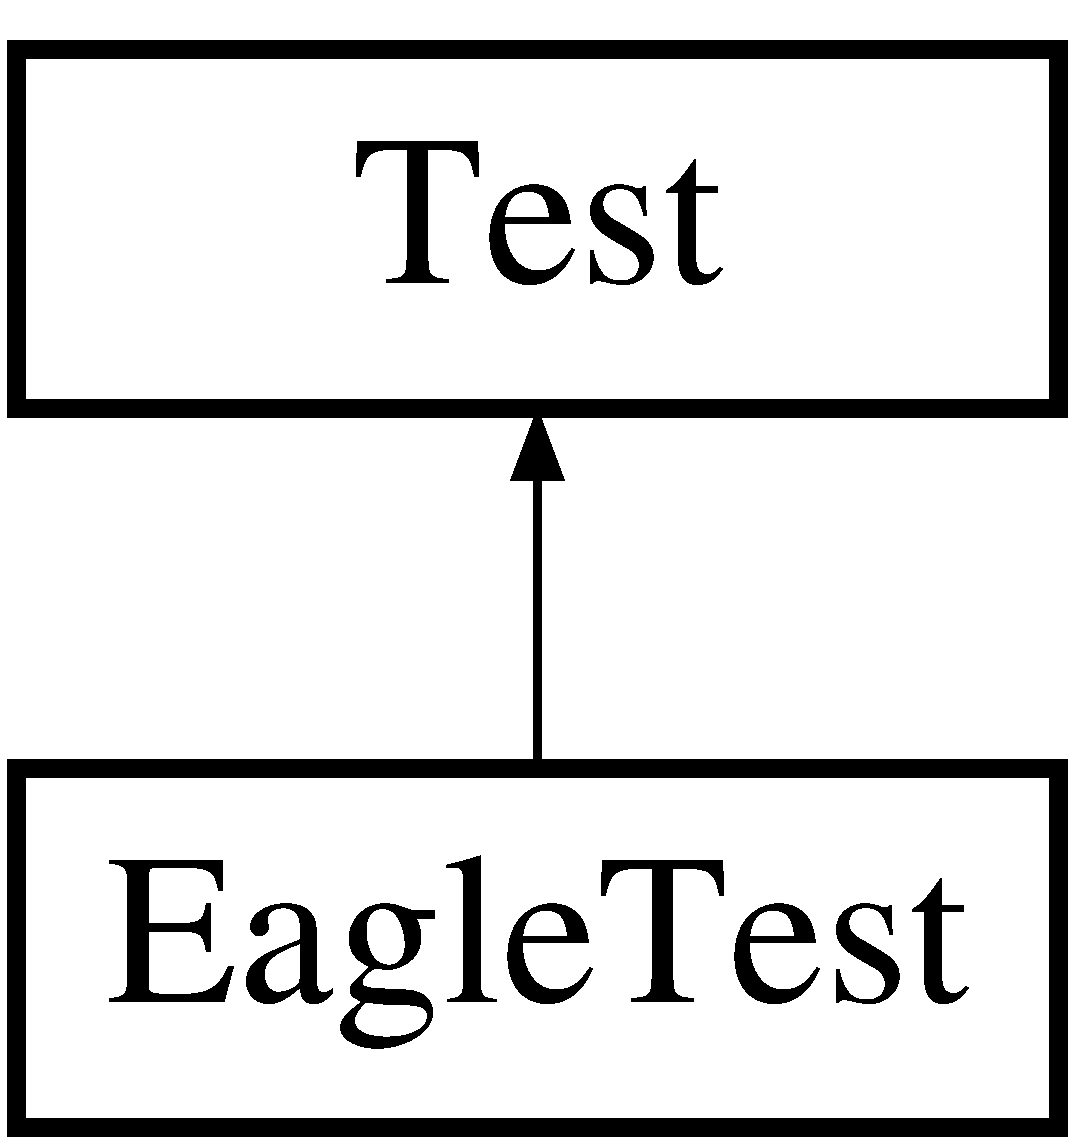
\includegraphics[height=2.000000cm]{class_eagle_test}
\end{center}
\end{figure}


The documentation for this class was generated from the following file\+:\begin{DoxyCompactItemize}
\item 
main\+\_\+test.\+cpp\end{DoxyCompactItemize}

\hypertarget{class_girrafe}{}\section{Girrafe Class Reference}
\label{class_girrafe}\index{Girrafe@{Girrafe}}
Inheritance diagram for Girrafe\+:\begin{figure}[H]
\begin{center}
\leavevmode
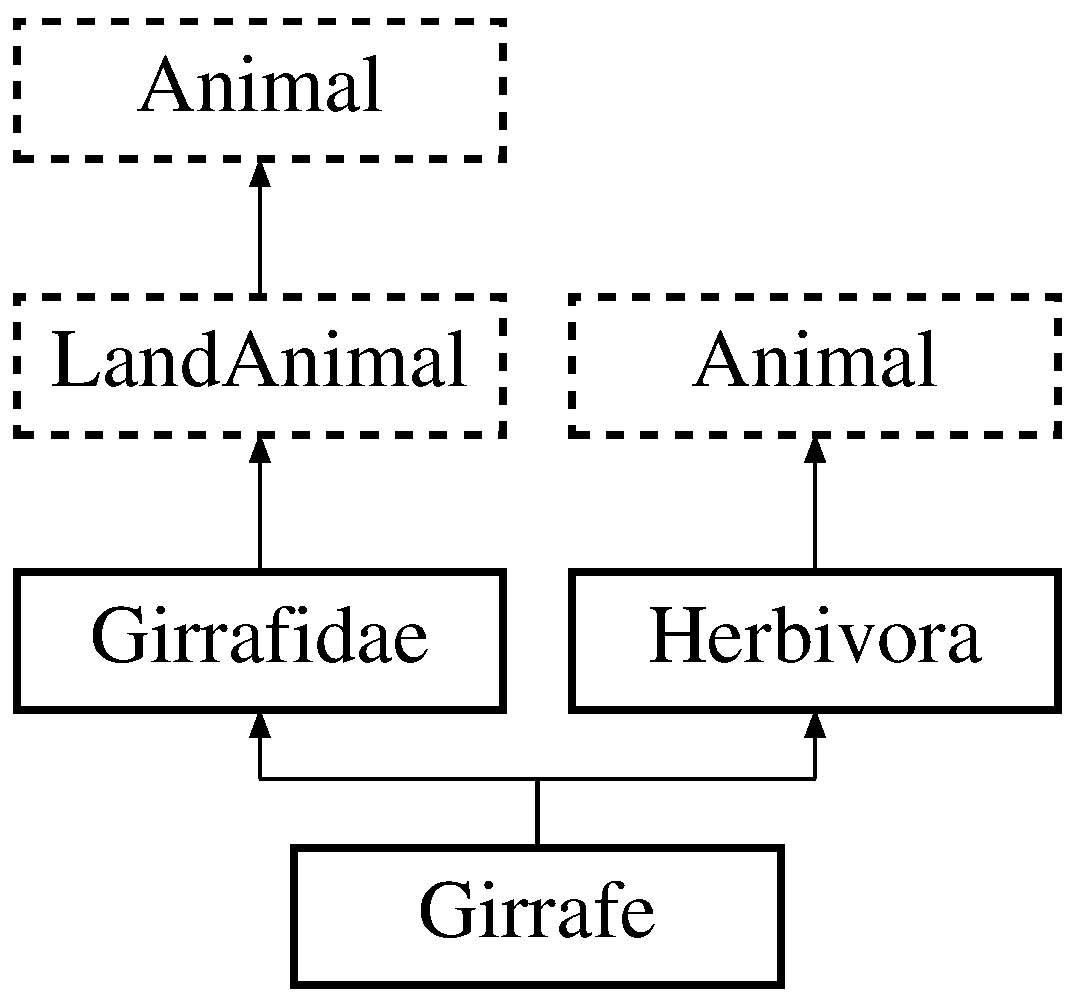
\includegraphics[height=4.000000cm]{class_girrafe}
\end{center}
\end{figure}
\subsection*{Public Member Functions}
\begin{DoxyCompactItemize}
\item 
\hyperlink{class_girrafe_a2f0f0d978d40addd7acb4c14f0080087}{Girrafe} ()\hypertarget{class_girrafe_a2f0f0d978d40addd7acb4c14f0080087}{}\label{class_girrafe_a2f0f0d978d40addd7acb4c14f0080087}

\begin{DoxyCompactList}\small\item\em Inisialisasi Hewan. \end{DoxyCompactList}\end{DoxyCompactItemize}
\subsection*{Additional Inherited Members}


The documentation for this class was generated from the following files\+:\begin{DoxyCompactItemize}
\item 
land\+\_\+animal.\+h\item 
land\+\_\+animal.\+cpp\end{DoxyCompactItemize}

\hypertarget{class_girrafe_test}{}\section{Girrafe\+Test Class Reference}
\label{class_girrafe_test}\index{Girrafe\+Test@{Girrafe\+Test}}
Inheritance diagram for Girrafe\+Test\+:\begin{figure}[H]
\begin{center}
\leavevmode
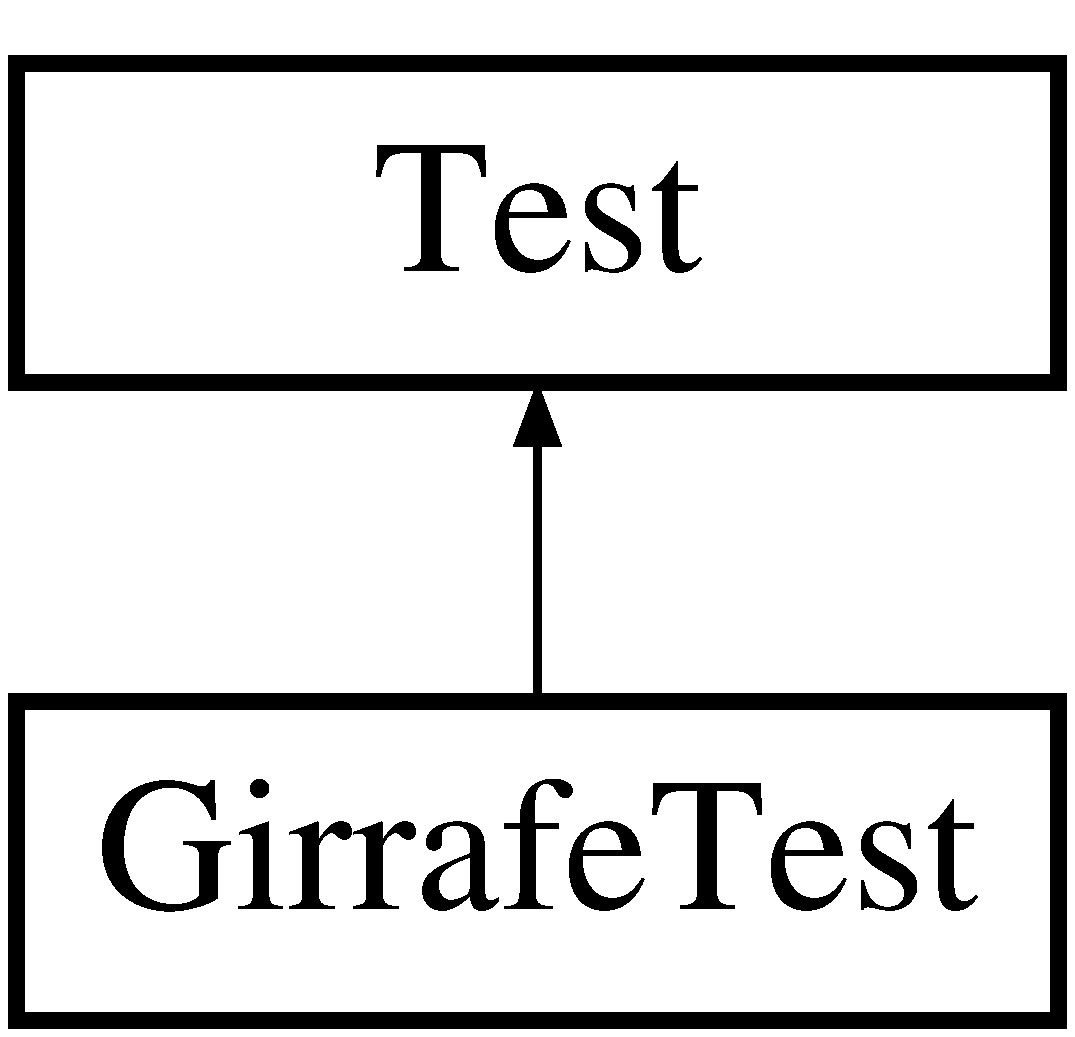
\includegraphics[height=2.000000cm]{class_girrafe_test}
\end{center}
\end{figure}


The documentation for this class was generated from the following file\+:\begin{DoxyCompactItemize}
\item 
main\+\_\+test.\+cpp\end{DoxyCompactItemize}

\hypertarget{class_gorilla}{}\section{Gorilla Class Reference}
\label{class_gorilla}\index{Gorilla@{Gorilla}}
Inheritance diagram for Gorilla\+:\begin{figure}[H]
\begin{center}
\leavevmode
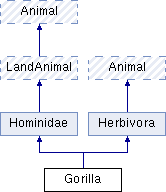
\includegraphics[height=4.000000cm]{class_gorilla}
\end{center}
\end{figure}
\subsection*{Public Member Functions}
\begin{DoxyCompactItemize}
\item 
\hyperlink{class_gorilla_a01f4f53de267d241d46256ce1bb3cc3a}{Gorilla} ()\hypertarget{class_gorilla_a01f4f53de267d241d46256ce1bb3cc3a}{}\label{class_gorilla_a01f4f53de267d241d46256ce1bb3cc3a}

\begin{DoxyCompactList}\small\item\em Inisialisasi Hewan. \end{DoxyCompactList}\end{DoxyCompactItemize}
\subsection*{Additional Inherited Members}


The documentation for this class was generated from the following files\+:\begin{DoxyCompactItemize}
\item 
land\+\_\+animal.\+h\item 
land\+\_\+animal.\+cpp\end{DoxyCompactItemize}

\hypertarget{class_gorilla_test}{}\section{Gorilla\+Test Class Reference}
\label{class_gorilla_test}\index{Gorilla\+Test@{Gorilla\+Test}}
Inheritance diagram for Gorilla\+Test\+:\begin{figure}[H]
\begin{center}
\leavevmode
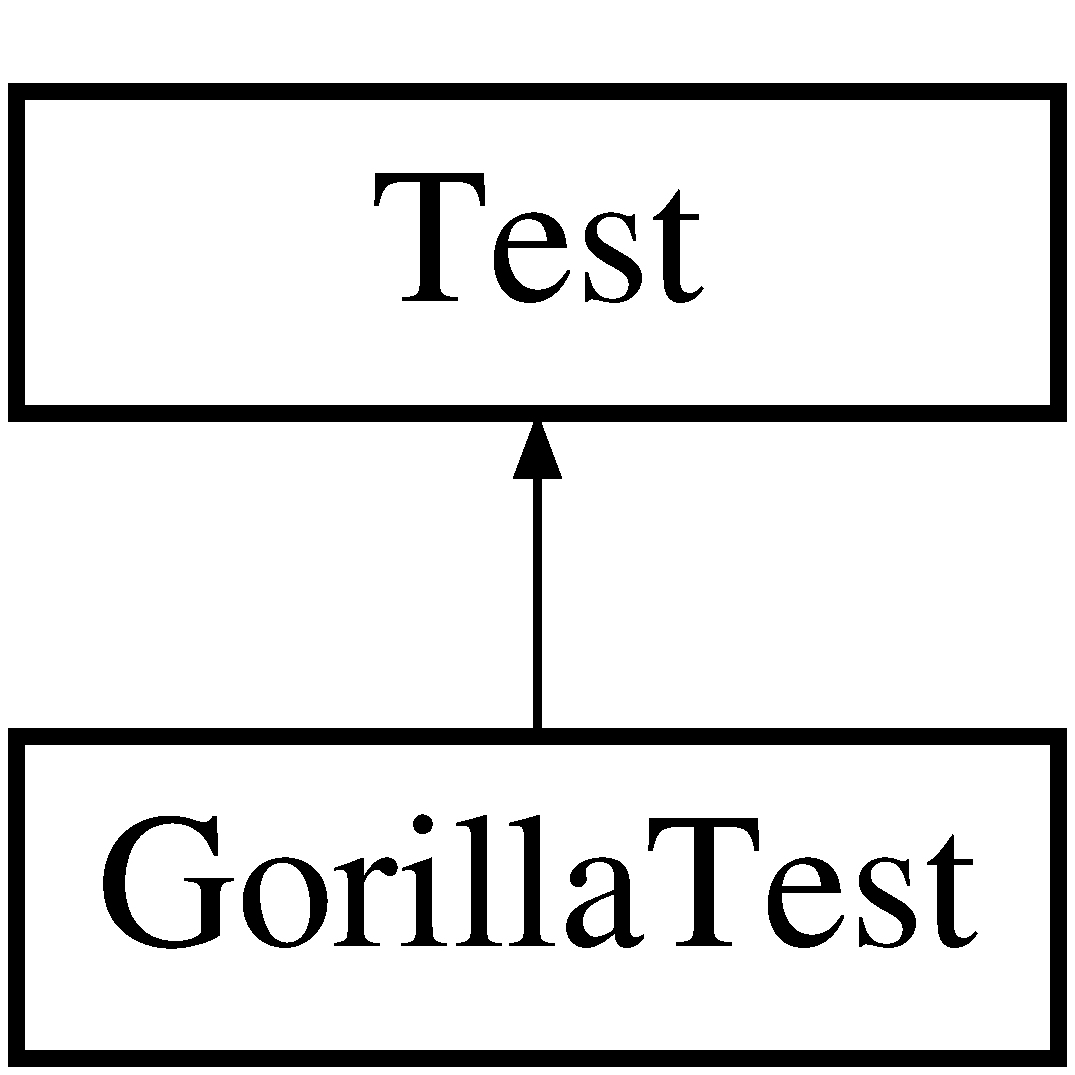
\includegraphics[height=2.000000cm]{class_gorilla_test}
\end{center}
\end{figure}


The documentation for this class was generated from the following file\+:\begin{DoxyCompactItemize}
\item 
main\+\_\+test.\+cpp\end{DoxyCompactItemize}

\hypertarget{class_indian_phyton}{}\section{Indian\+Phyton Class Reference}
\label{class_indian_phyton}\index{Indian\+Phyton@{Indian\+Phyton}}
\subsection*{Public Member Functions}
\begin{DoxyCompactItemize}
\item 
\hyperlink{class_indian_phyton_ac10885d0edb63c66f897ced1e7af87d4}{Indian\+Phyton} ()\hypertarget{class_indian_phyton_ac10885d0edb63c66f897ced1e7af87d4}{}\label{class_indian_phyton_ac10885d0edb63c66f897ced1e7af87d4}

\begin{DoxyCompactList}\small\item\em Constructor. \end{DoxyCompactList}\item 
\hyperlink{class_indian_phyton_aa22d4887553ad6fe5cd120c2ae8b953e}{$\sim$\+Indian\+Phyton} ()\hypertarget{class_indian_phyton_aa22d4887553ad6fe5cd120c2ae8b953e}{}\label{class_indian_phyton_aa22d4887553ad6fe5cd120c2ae8b953e}

\begin{DoxyCompactList}\small\item\em Destructor. \end{DoxyCompactList}\item 
string \hyperlink{class_indian_phyton_aeea982676d703fda0dff1c8d6661db81}{Get\+Experience} ()\hypertarget{class_indian_phyton_aeea982676d703fda0dff1c8d6661db81}{}\label{class_indian_phyton_aeea982676d703fda0dff1c8d6661db81}

\begin{DoxyCompactList}\small\item\em Komunikasi dengan hewan. \end{DoxyCompactList}\item 
int \hyperlink{class_indian_phyton_a2ccd63f4aa5ac5e3da05e957331c875e}{Get\+Food\+Num} ()
\begin{DoxyCompactList}\small\item\em Jumlah makanan. \end{DoxyCompactList}\item 
char \hyperlink{class_indian_phyton_a336a8f1b7bc0e7f373c7e015f52991b7}{Get\+Render} ()
\begin{DoxyCompactList}\small\item\em Print karakter. \end{DoxyCompactList}\item 
void \hyperlink{class_indian_phyton_a38b4af678533080e63697115ec492d03}{Set\+Enemy} (char cc)
\begin{DoxyCompactList}\small\item\em Set karakter hewan. \end{DoxyCompactList}\item 
char $\ast$ \hyperlink{class_indian_phyton_afb15d6bd5b66f6a2104765253c4e0557}{Get\+Enemy} ()
\begin{DoxyCompactList}\small\item\em Ambil list musuh. \end{DoxyCompactList}\end{DoxyCompactItemize}
\subsection*{Protected Attributes}
\begin{DoxyCompactItemize}
\item 
int $\ast$ \hyperlink{class_indian_phyton_a9798f27b0e5331587f03adb240deb1df}{Type}
\item 
string \hyperlink{class_indian_phyton_ab5aea03e94363bd76ffa575c66218a55}{Famili}
\item 
string \hyperlink{class_indian_phyton_a4c140a1de8195f136530bb8ea148e33f}{Species}
\item 
string \hyperlink{class_indian_phyton_a6127b783d74687a90aaa2ec962ddb316}{Experience}
\item 
short \hyperlink{class_indian_phyton_adef9db8c3e643bb0eee4bdaf6a81c06b}{Jenis\+Makanan}
\item 
int \hyperlink{class_indian_phyton_ab2bedace1b95a7961ca9033d364b39c8}{Berat}
\item 
char \hyperlink{class_indian_phyton_a200d15945544e1f74a4ae1e5507ad0aa}{Ani\+Char}
\item 
char $\ast$ \hyperlink{class_indian_phyton_a369222c3fe97923ff7b08300ae8833ad}{Enemy\+Char}
\item 
int \hyperlink{class_indian_phyton_ada8efc5d65c3c36a9b2f4c422893810c}{Top\+Enemy}
\end{DoxyCompactItemize}


\subsection{Member Function Documentation}
\index{Indian\+Phyton@{Indian\+Phyton}!Get\+Enemy@{Get\+Enemy}}
\index{Get\+Enemy@{Get\+Enemy}!Indian\+Phyton@{Indian\+Phyton}}
\subsubsection[{\texorpdfstring{Get\+Enemy()}{GetEnemy()}}]{\setlength{\rightskip}{0pt plus 5cm}char $\ast$ Indian\+Phyton\+::\+Get\+Enemy (
\begin{DoxyParamCaption}
{}
\end{DoxyParamCaption}
)}\hypertarget{class_indian_phyton_afb15d6bd5b66f6a2104765253c4e0557}{}\label{class_indian_phyton_afb15d6bd5b66f6a2104765253c4e0557}


Ambil list musuh. 

\begin{DoxyReturn}{Returns}
List Musuh 
\end{DoxyReturn}
\index{Indian\+Phyton@{Indian\+Phyton}!Get\+Food\+Num@{Get\+Food\+Num}}
\index{Get\+Food\+Num@{Get\+Food\+Num}!Indian\+Phyton@{Indian\+Phyton}}
\subsubsection[{\texorpdfstring{Get\+Food\+Num()}{GetFoodNum()}}]{\setlength{\rightskip}{0pt plus 5cm}int Indian\+Phyton\+::\+Get\+Food\+Num (
\begin{DoxyParamCaption}
{}
\end{DoxyParamCaption}
)}\hypertarget{class_indian_phyton_a2ccd63f4aa5ac5e3da05e957331c875e}{}\label{class_indian_phyton_a2ccd63f4aa5ac5e3da05e957331c875e}


Jumlah makanan. 

\begin{DoxyReturn}{Returns}
Jumlah makan

Jumlah makanan 
\end{DoxyReturn}
\index{Indian\+Phyton@{Indian\+Phyton}!Get\+Render@{Get\+Render}}
\index{Get\+Render@{Get\+Render}!Indian\+Phyton@{Indian\+Phyton}}
\subsubsection[{\texorpdfstring{Get\+Render()}{GetRender()}}]{\setlength{\rightskip}{0pt plus 5cm}char Indian\+Phyton\+::\+Get\+Render (
\begin{DoxyParamCaption}
{}
\end{DoxyParamCaption}
)}\hypertarget{class_indian_phyton_a336a8f1b7bc0e7f373c7e015f52991b7}{}\label{class_indian_phyton_a336a8f1b7bc0e7f373c7e015f52991b7}


Print karakter. 

\begin{DoxyReturn}{Returns}
char 
\end{DoxyReturn}
\index{Indian\+Phyton@{Indian\+Phyton}!Set\+Enemy@{Set\+Enemy}}
\index{Set\+Enemy@{Set\+Enemy}!Indian\+Phyton@{Indian\+Phyton}}
\subsubsection[{\texorpdfstring{Set\+Enemy(char cc)}{SetEnemy(char cc)}}]{\setlength{\rightskip}{0pt plus 5cm}void Indian\+Phyton\+::\+Set\+Enemy (
\begin{DoxyParamCaption}
\item[{char}]{cc}
\end{DoxyParamCaption}
)}\hypertarget{class_indian_phyton_a38b4af678533080e63697115ec492d03}{}\label{class_indian_phyton_a38b4af678533080e63697115ec492d03}


Set karakter hewan. 


\begin{DoxyParams}{Parameters}
{\em cc} & Karakter hewan tsb \\
\hline
\end{DoxyParams}


\subsection{Member Data Documentation}
\index{Indian\+Phyton@{Indian\+Phyton}!Ani\+Char@{Ani\+Char}}
\index{Ani\+Char@{Ani\+Char}!Indian\+Phyton@{Indian\+Phyton}}
\subsubsection[{\texorpdfstring{Ani\+Char}{AniChar}}]{\setlength{\rightskip}{0pt plus 5cm}char Indian\+Phyton\+::\+Ani\+Char\hspace{0.3cm}{\ttfamily [protected]}}\hypertarget{class_indian_phyton_a200d15945544e1f74a4ae1e5507ad0aa}{}\label{class_indian_phyton_a200d15945544e1f74a4ae1e5507ad0aa}
Char yang digunakan untuk render \index{Indian\+Phyton@{Indian\+Phyton}!Berat@{Berat}}
\index{Berat@{Berat}!Indian\+Phyton@{Indian\+Phyton}}
\subsubsection[{\texorpdfstring{Berat}{Berat}}]{\setlength{\rightskip}{0pt plus 5cm}int Indian\+Phyton\+::\+Berat\hspace{0.3cm}{\ttfamily [protected]}}\hypertarget{class_indian_phyton_ab2bedace1b95a7961ca9033d364b39c8}{}\label{class_indian_phyton_ab2bedace1b95a7961ca9033d364b39c8}
Berat hewan \index{Indian\+Phyton@{Indian\+Phyton}!Enemy\+Char@{Enemy\+Char}}
\index{Enemy\+Char@{Enemy\+Char}!Indian\+Phyton@{Indian\+Phyton}}
\subsubsection[{\texorpdfstring{Enemy\+Char}{EnemyChar}}]{\setlength{\rightskip}{0pt plus 5cm}char$\ast$ Indian\+Phyton\+::\+Enemy\+Char\hspace{0.3cm}{\ttfamily [protected]}}\hypertarget{class_indian_phyton_a369222c3fe97923ff7b08300ae8833ad}{}\label{class_indian_phyton_a369222c3fe97923ff7b08300ae8833ad}
Array of char yang berisi list musuhnya \index{Indian\+Phyton@{Indian\+Phyton}!Experience@{Experience}}
\index{Experience@{Experience}!Indian\+Phyton@{Indian\+Phyton}}
\subsubsection[{\texorpdfstring{Experience}{Experience}}]{\setlength{\rightskip}{0pt plus 5cm}string Indian\+Phyton\+::\+Experience\hspace{0.3cm}{\ttfamily [protected]}}\hypertarget{class_indian_phyton_a6127b783d74687a90aaa2ec962ddb316}{}\label{class_indian_phyton_a6127b783d74687a90aaa2ec962ddb316}
Experience hewan \index{Indian\+Phyton@{Indian\+Phyton}!Famili@{Famili}}
\index{Famili@{Famili}!Indian\+Phyton@{Indian\+Phyton}}
\subsubsection[{\texorpdfstring{Famili}{Famili}}]{\setlength{\rightskip}{0pt plus 5cm}string Indian\+Phyton\+::\+Famili\hspace{0.3cm}{\ttfamily [protected]}}\hypertarget{class_indian_phyton_ab5aea03e94363bd76ffa575c66218a55}{}\label{class_indian_phyton_ab5aea03e94363bd76ffa575c66218a55}
Family hewan \index{Indian\+Phyton@{Indian\+Phyton}!Jenis\+Makanan@{Jenis\+Makanan}}
\index{Jenis\+Makanan@{Jenis\+Makanan}!Indian\+Phyton@{Indian\+Phyton}}
\subsubsection[{\texorpdfstring{Jenis\+Makanan}{JenisMakanan}}]{\setlength{\rightskip}{0pt plus 5cm}short Indian\+Phyton\+::\+Jenis\+Makanan\hspace{0.3cm}{\ttfamily [protected]}}\hypertarget{class_indian_phyton_adef9db8c3e643bb0eee4bdaf6a81c06b}{}\label{class_indian_phyton_adef9db8c3e643bb0eee4bdaf6a81c06b}
Jenis Makanan hewan. 1 \+: herbifor, 2 \+: karnivor, 3 \+: omnifor \index{Indian\+Phyton@{Indian\+Phyton}!Species@{Species}}
\index{Species@{Species}!Indian\+Phyton@{Indian\+Phyton}}
\subsubsection[{\texorpdfstring{Species}{Species}}]{\setlength{\rightskip}{0pt plus 5cm}string Indian\+Phyton\+::\+Species\hspace{0.3cm}{\ttfamily [protected]}}\hypertarget{class_indian_phyton_a4c140a1de8195f136530bb8ea148e33f}{}\label{class_indian_phyton_a4c140a1de8195f136530bb8ea148e33f}
Species hewan \index{Indian\+Phyton@{Indian\+Phyton}!Top\+Enemy@{Top\+Enemy}}
\index{Top\+Enemy@{Top\+Enemy}!Indian\+Phyton@{Indian\+Phyton}}
\subsubsection[{\texorpdfstring{Top\+Enemy}{TopEnemy}}]{\setlength{\rightskip}{0pt plus 5cm}int Indian\+Phyton\+::\+Top\+Enemy\hspace{0.3cm}{\ttfamily [protected]}}\hypertarget{class_indian_phyton_ada8efc5d65c3c36a9b2f4c422893810c}{}\label{class_indian_phyton_ada8efc5d65c3c36a9b2f4c422893810c}
Pointer Enemy\+Char yang available \index{Indian\+Phyton@{Indian\+Phyton}!Type@{Type}}
\index{Type@{Type}!Indian\+Phyton@{Indian\+Phyton}}
\subsubsection[{\texorpdfstring{Type}{Type}}]{\setlength{\rightskip}{0pt plus 5cm}int$\ast$ Indian\+Phyton\+::\+Type\hspace{0.3cm}{\ttfamily [protected]}}\hypertarget{class_indian_phyton_a9798f27b0e5331587f03adb240deb1df}{}\label{class_indian_phyton_a9798f27b0e5331587f03adb240deb1df}
Type habitat hewan. 0 \+: darat, 1 \+: udara, 2 \+: air 

The documentation for this class was generated from the following files\+:\begin{DoxyCompactItemize}
\item 
indianphyton.\+h\item 
indianphyton.\+cpp\end{DoxyCompactItemize}

\hypertarget{class_indian_phyton_test}{}\section{Indian\+Phyton\+Test Class Reference}
\label{class_indian_phyton_test}\index{Indian\+Phyton\+Test@{Indian\+Phyton\+Test}}
Inheritance diagram for Indian\+Phyton\+Test\+:\begin{figure}[H]
\begin{center}
\leavevmode
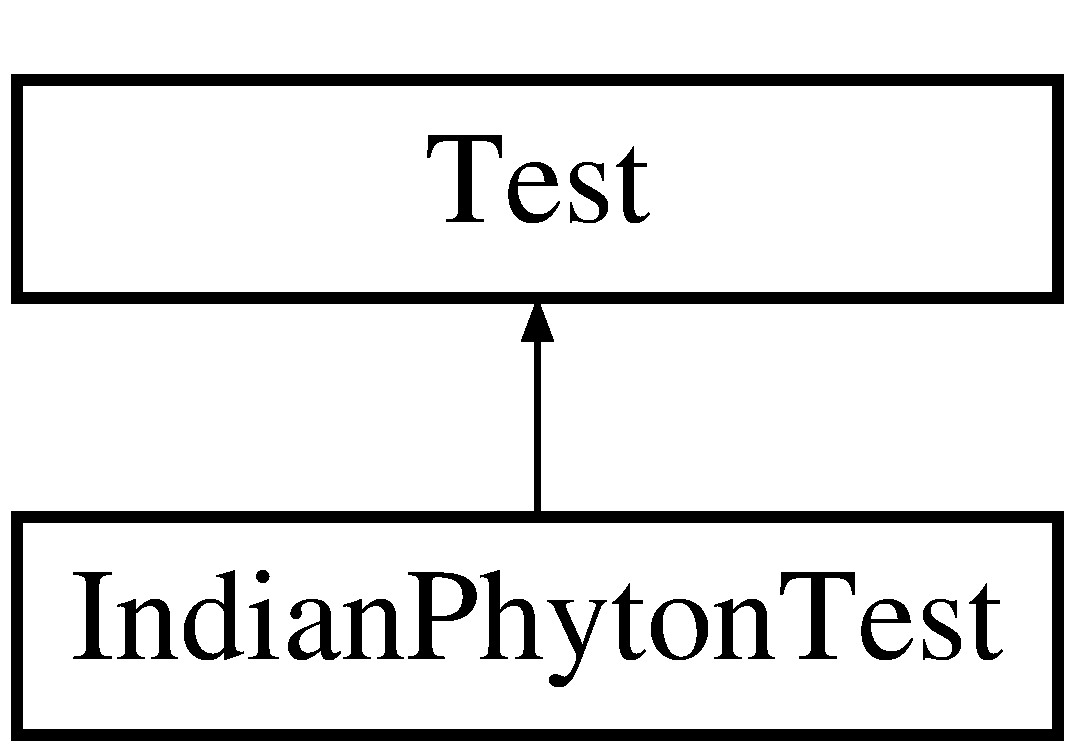
\includegraphics[height=2.000000cm]{class_indian_phyton_test}
\end{center}
\end{figure}


The documentation for this class was generated from the following file\+:\begin{DoxyCompactItemize}
\item 
main\+\_\+test.\+cpp\end{DoxyCompactItemize}

\hypertarget{class_land_habitat}{}\section{Land\+Habitat Class Reference}
\label{class_land_habitat}\index{Land\+Habitat@{Land\+Habitat}}
\subsection*{Public Member Functions}
\begin{DoxyCompactItemize}
\item 
\hyperlink{class_land_habitat_afa67ffdf6984ec7c1fcc6ec27d5628d3}{Land\+Habitat} ()
\begin{DoxyCompactList}\small\item\em constructor \end{DoxyCompactList}\item 
virtual \hyperlink{class_land_habitat_a0c1aebc080f875b9053f3a776aea627a}{$\sim$\+Land\+Habitat} ()\hypertarget{class_land_habitat_a0c1aebc080f875b9053f3a776aea627a}{}\label{class_land_habitat_a0c1aebc080f875b9053f3a776aea627a}

\begin{DoxyCompactList}\small\item\em Destructor. \end{DoxyCompactList}\item 
char \hyperlink{class_land_habitat_af338ed3cae85590e9a5f74d94913ebf8}{Get\+Render} ()
\begin{DoxyCompactList}\small\item\em render nawn \end{DoxyCompactList}\end{DoxyCompactItemize}


\subsection{Constructor \& Destructor Documentation}
\index{Land\+Habitat@{Land\+Habitat}!Land\+Habitat@{Land\+Habitat}}
\index{Land\+Habitat@{Land\+Habitat}!Land\+Habitat@{Land\+Habitat}}
\subsubsection[{\texorpdfstring{Land\+Habitat()}{LandHabitat()}}]{\setlength{\rightskip}{0pt plus 5cm}Land\+Habitat\+::\+Land\+Habitat (
\begin{DoxyParamCaption}
{}
\end{DoxyParamCaption}
)}\hypertarget{class_land_habitat_afa67ffdf6984ec7c1fcc6ec27d5628d3}{}\label{class_land_habitat_afa67ffdf6984ec7c1fcc6ec27d5628d3}


constructor 


\begin{DoxyParams}{Parameters}
{\em posx} & posisi x \\
\hline
{\em posy} & posisi y \\
\hline
\end{DoxyParams}


\subsection{Member Function Documentation}
\index{Land\+Habitat@{Land\+Habitat}!Get\+Render@{Get\+Render}}
\index{Get\+Render@{Get\+Render}!Land\+Habitat@{Land\+Habitat}}
\subsubsection[{\texorpdfstring{Get\+Render()}{GetRender()}}]{\setlength{\rightskip}{0pt plus 5cm}char Land\+Habitat\+::\+Get\+Render (
\begin{DoxyParamCaption}
{}
\end{DoxyParamCaption}
)}\hypertarget{class_land_habitat_af338ed3cae85590e9a5f74d94913ebf8}{}\label{class_land_habitat_af338ed3cae85590e9a5f74d94913ebf8}


render nawn 


\begin{DoxyParams}{Parameters}
{\em cc} & nawnnawn \\
\hline
\end{DoxyParams}


The documentation for this class was generated from the following files\+:\begin{DoxyCompactItemize}
\item 
land\+\_\+habitat.\+h\item 
land\+\_\+habitat.\+cpp\end{DoxyCompactItemize}

\hypertarget{class_land_habitat_test}{}\section{Land\+Habitat\+Test Class Reference}
\label{class_land_habitat_test}\index{Land\+Habitat\+Test@{Land\+Habitat\+Test}}
Inheritance diagram for Land\+Habitat\+Test\+:\begin{figure}[H]
\begin{center}
\leavevmode
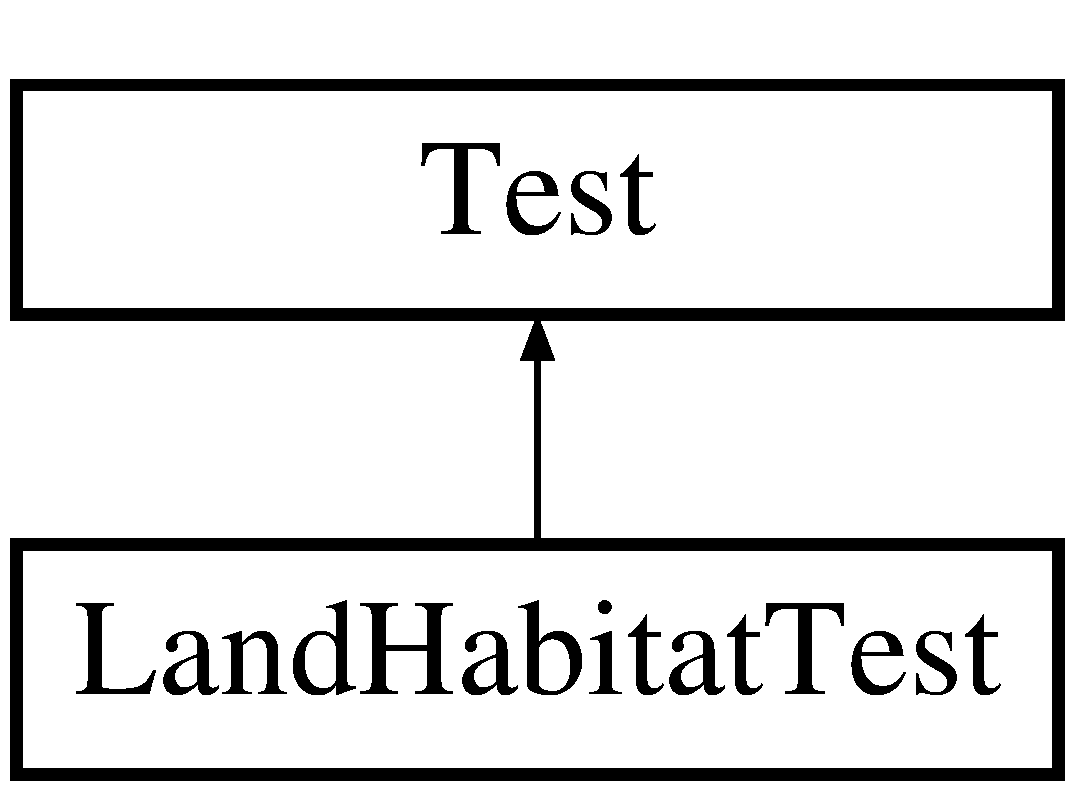
\includegraphics[height=2.000000cm]{class_land_habitat_test}
\end{center}
\end{figure}


The documentation for this class was generated from the following file\+:\begin{DoxyCompactItemize}
\item 
main\+\_\+test.\+cpp\end{DoxyCompactItemize}

\hypertarget{class_lion}{}\section{Lion Class Reference}
\label{class_lion}\index{Lion@{Lion}}
Inheritance diagram for Lion\+:\begin{figure}[H]
\begin{center}
\leavevmode
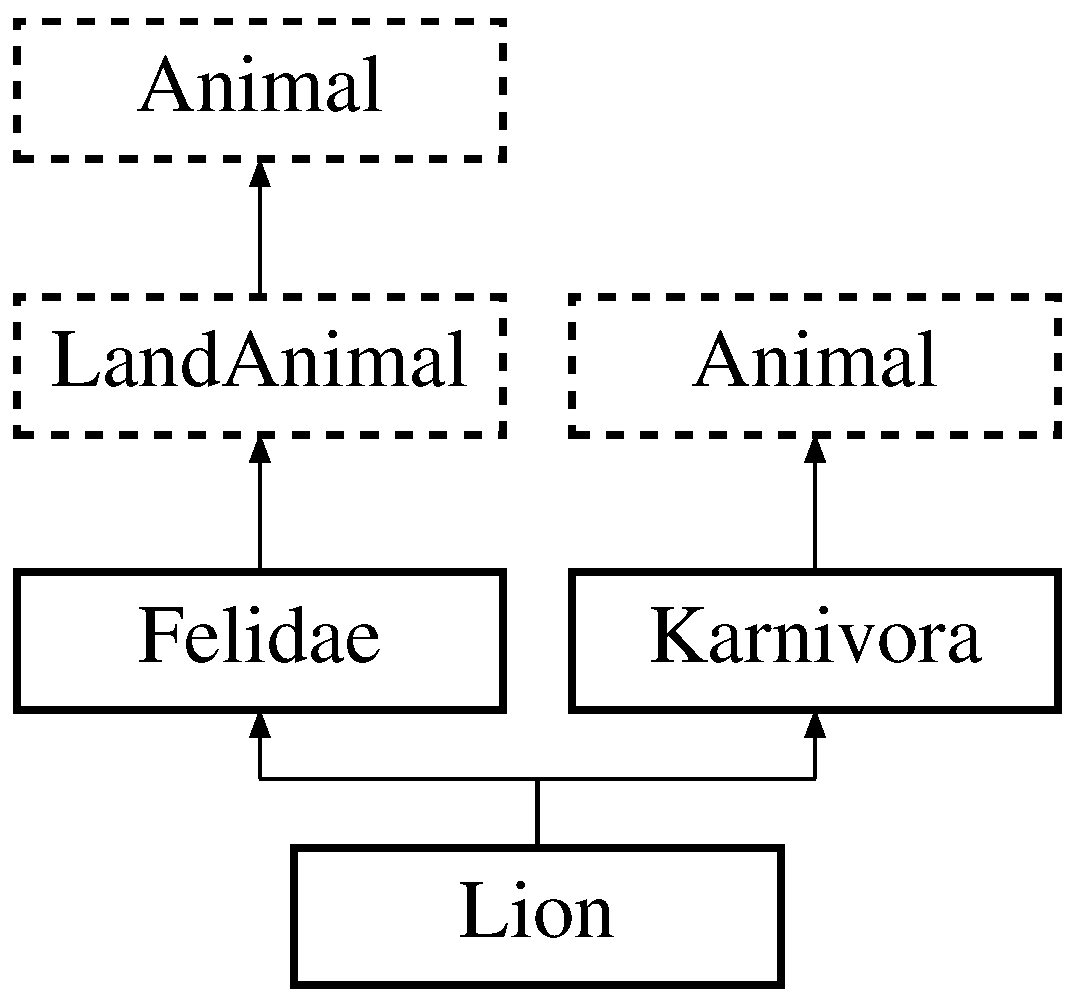
\includegraphics[height=4.000000cm]{class_lion}
\end{center}
\end{figure}
\subsection*{Public Member Functions}
\begin{DoxyCompactItemize}
\item 
\hyperlink{class_lion_a582202364024a9ce10e57f47c872dbc2}{Lion} ()\hypertarget{class_lion_a582202364024a9ce10e57f47c872dbc2}{}\label{class_lion_a582202364024a9ce10e57f47c872dbc2}

\begin{DoxyCompactList}\small\item\em Inisialisasi Hewan. \end{DoxyCompactList}\end{DoxyCompactItemize}
\subsection*{Additional Inherited Members}


The documentation for this class was generated from the following files\+:\begin{DoxyCompactItemize}
\item 
land\+\_\+animal.\+h\item 
land\+\_\+animal.\+cpp\end{DoxyCompactItemize}

\hypertarget{class_lion_test}{}\section{Lion\+Test Class Reference}
\label{class_lion_test}\index{Lion\+Test@{Lion\+Test}}
Inheritance diagram for Lion\+Test\+:\begin{figure}[H]
\begin{center}
\leavevmode
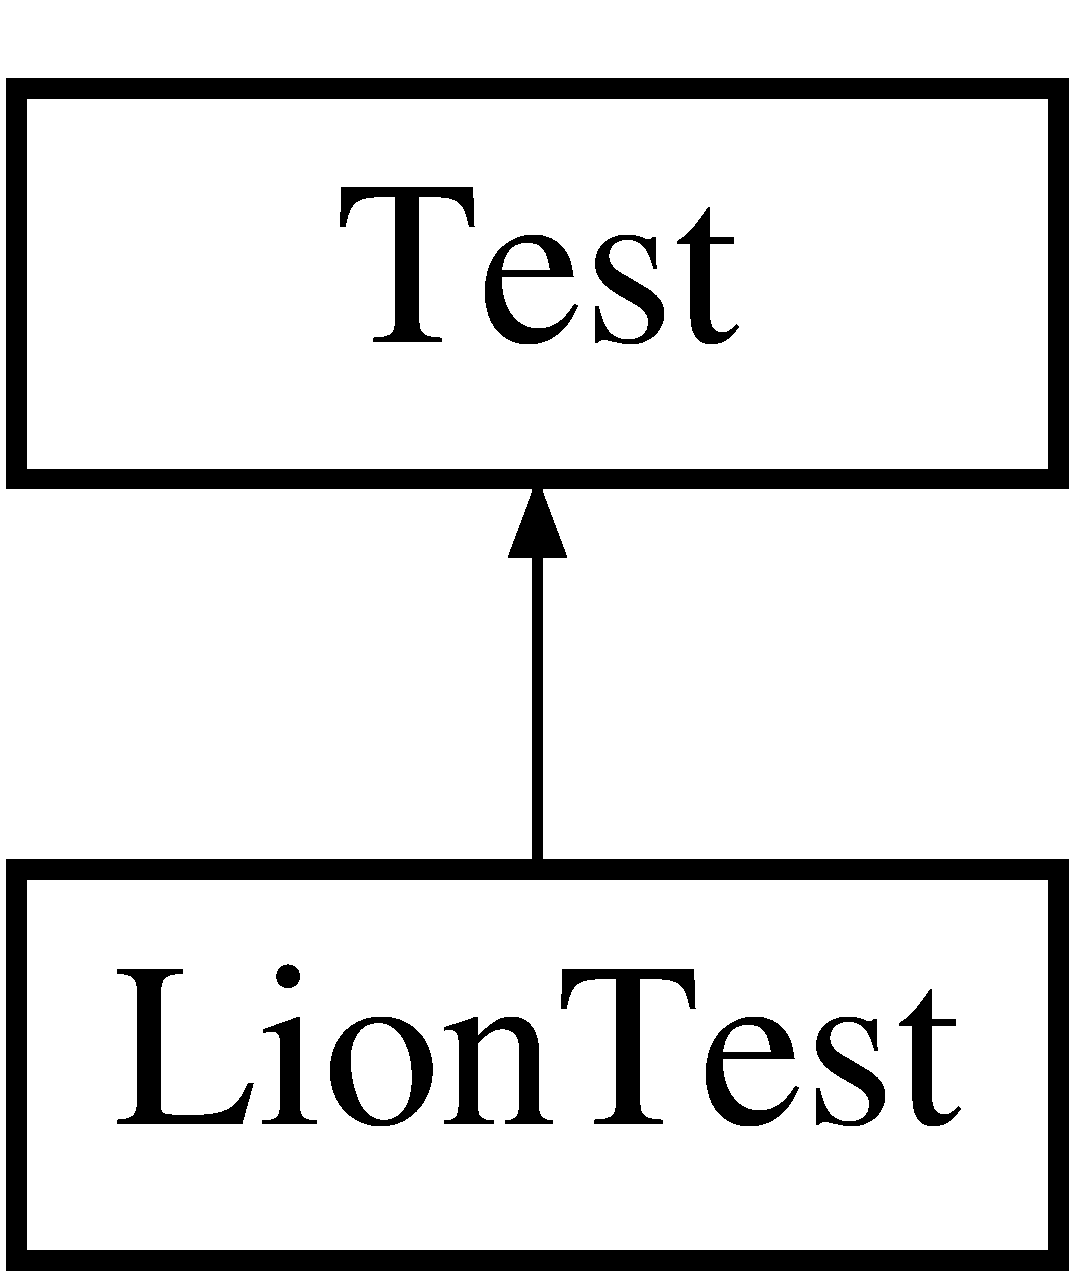
\includegraphics[height=2.000000cm]{class_lion_test}
\end{center}
\end{figure}


The documentation for this class was generated from the following file\+:\begin{DoxyCompactItemize}
\item 
main\+\_\+test.\+cpp\end{DoxyCompactItemize}

\hypertarget{class_merak}{}\section{Merak Class Reference}
\label{class_merak}\index{Merak@{Merak}}
\subsection*{Public Member Functions}
\begin{DoxyCompactItemize}
\item 
\hyperlink{class_merak_abc8e0d235b1fadd0e522f2e8f84677e6}{Merak} ()\hypertarget{class_merak_abc8e0d235b1fadd0e522f2e8f84677e6}{}\label{class_merak_abc8e0d235b1fadd0e522f2e8f84677e6}

\begin{DoxyCompactList}\small\item\em Constructor. \end{DoxyCompactList}\item 
\hyperlink{class_merak_a022375e5e76dda9db65d6d46b217eee1}{$\sim$\+Merak} ()\hypertarget{class_merak_a022375e5e76dda9db65d6d46b217eee1}{}\label{class_merak_a022375e5e76dda9db65d6d46b217eee1}

\begin{DoxyCompactList}\small\item\em Destructor. \end{DoxyCompactList}\item 
string \hyperlink{class_merak_aecc0ca605df25195981f2faeb354b8e2}{Get\+Experience} ()\hypertarget{class_merak_aecc0ca605df25195981f2faeb354b8e2}{}\label{class_merak_aecc0ca605df25195981f2faeb354b8e2}

\begin{DoxyCompactList}\small\item\em Komunikasi dengan hewan. \end{DoxyCompactList}\item 
int \hyperlink{class_merak_a26c1ae4b0ee2781c6f601b5e22deecc6}{Get\+Food\+Num} ()
\begin{DoxyCompactList}\small\item\em Jumlah makanan. \end{DoxyCompactList}\item 
char \hyperlink{class_merak_a7f39bd60fe12f24769d1f2bf42b1fdd7}{Get\+Render} ()
\begin{DoxyCompactList}\small\item\em Print karakter. \end{DoxyCompactList}\item 
void \hyperlink{class_merak_a68c00568fab98e4e02ec4a84bb582463}{Set\+Enemy} (char cc)
\begin{DoxyCompactList}\small\item\em Set karakter hewan. \end{DoxyCompactList}\item 
char $\ast$ \hyperlink{class_merak_aec4d007180b1f9dc20ed95e9e6736c00}{Get\+Enemy} ()
\begin{DoxyCompactList}\small\item\em Ambil list musuh. \end{DoxyCompactList}\end{DoxyCompactItemize}
\subsection*{Protected Attributes}
\begin{DoxyCompactItemize}
\item 
int $\ast$ \hyperlink{class_merak_afc4c29c5ceae86542a54c8f73445097e}{Type}
\item 
string \hyperlink{class_merak_ab8646f355a3376626fa1dcb65c01e05c}{Famili}
\item 
string \hyperlink{class_merak_a93a71597be852ba02e83e5ae8d34c115}{Species}
\item 
string \hyperlink{class_merak_a6e1062918be8574174f82425620eb18b}{Experience}
\item 
short \hyperlink{class_merak_a167f51348667b9244da278b166a883bd}{Jenis\+Makanan}
\item 
int \hyperlink{class_merak_a4bb6302bfe501ef6286147ea7f003a09}{Berat}
\item 
char \hyperlink{class_merak_a06809533984c3907e6c8c517273b1ba4}{Ani\+Char}
\item 
char $\ast$ \hyperlink{class_merak_aae4b84ebb17b158fd1f2c0d9a974d62a}{Enemy\+Char}
\item 
int \hyperlink{class_merak_ace55be82878a446afa663c843b7aedc1}{Top\+Enemy}
\end{DoxyCompactItemize}


\subsection{Member Function Documentation}
\index{Merak@{Merak}!Get\+Enemy@{Get\+Enemy}}
\index{Get\+Enemy@{Get\+Enemy}!Merak@{Merak}}
\subsubsection[{\texorpdfstring{Get\+Enemy()}{GetEnemy()}}]{\setlength{\rightskip}{0pt plus 5cm}char $\ast$ Merak\+::\+Get\+Enemy (
\begin{DoxyParamCaption}
{}
\end{DoxyParamCaption}
)}\hypertarget{class_merak_aec4d007180b1f9dc20ed95e9e6736c00}{}\label{class_merak_aec4d007180b1f9dc20ed95e9e6736c00}


Ambil list musuh. 

\begin{DoxyReturn}{Returns}
List Musuh 
\end{DoxyReturn}
\index{Merak@{Merak}!Get\+Food\+Num@{Get\+Food\+Num}}
\index{Get\+Food\+Num@{Get\+Food\+Num}!Merak@{Merak}}
\subsubsection[{\texorpdfstring{Get\+Food\+Num()}{GetFoodNum()}}]{\setlength{\rightskip}{0pt plus 5cm}int Merak\+::\+Get\+Food\+Num (
\begin{DoxyParamCaption}
{}
\end{DoxyParamCaption}
)}\hypertarget{class_merak_a26c1ae4b0ee2781c6f601b5e22deecc6}{}\label{class_merak_a26c1ae4b0ee2781c6f601b5e22deecc6}


Jumlah makanan. 

\begin{DoxyReturn}{Returns}
Jumlah makan

Jumlah makanan 
\end{DoxyReturn}
\index{Merak@{Merak}!Get\+Render@{Get\+Render}}
\index{Get\+Render@{Get\+Render}!Merak@{Merak}}
\subsubsection[{\texorpdfstring{Get\+Render()}{GetRender()}}]{\setlength{\rightskip}{0pt plus 5cm}char Merak\+::\+Get\+Render (
\begin{DoxyParamCaption}
{}
\end{DoxyParamCaption}
)}\hypertarget{class_merak_a7f39bd60fe12f24769d1f2bf42b1fdd7}{}\label{class_merak_a7f39bd60fe12f24769d1f2bf42b1fdd7}


Print karakter. 

\begin{DoxyReturn}{Returns}
char 
\end{DoxyReturn}
\index{Merak@{Merak}!Set\+Enemy@{Set\+Enemy}}
\index{Set\+Enemy@{Set\+Enemy}!Merak@{Merak}}
\subsubsection[{\texorpdfstring{Set\+Enemy(char cc)}{SetEnemy(char cc)}}]{\setlength{\rightskip}{0pt plus 5cm}void Merak\+::\+Set\+Enemy (
\begin{DoxyParamCaption}
\item[{char}]{cc}
\end{DoxyParamCaption}
)}\hypertarget{class_merak_a68c00568fab98e4e02ec4a84bb582463}{}\label{class_merak_a68c00568fab98e4e02ec4a84bb582463}


Set karakter hewan. 


\begin{DoxyParams}{Parameters}
{\em cc} & Karakter hewan tsb \\
\hline
\end{DoxyParams}


\subsection{Member Data Documentation}
\index{Merak@{Merak}!Ani\+Char@{Ani\+Char}}
\index{Ani\+Char@{Ani\+Char}!Merak@{Merak}}
\subsubsection[{\texorpdfstring{Ani\+Char}{AniChar}}]{\setlength{\rightskip}{0pt plus 5cm}char Merak\+::\+Ani\+Char\hspace{0.3cm}{\ttfamily [protected]}}\hypertarget{class_merak_a06809533984c3907e6c8c517273b1ba4}{}\label{class_merak_a06809533984c3907e6c8c517273b1ba4}
Char yang digunakan untuk render \index{Merak@{Merak}!Berat@{Berat}}
\index{Berat@{Berat}!Merak@{Merak}}
\subsubsection[{\texorpdfstring{Berat}{Berat}}]{\setlength{\rightskip}{0pt plus 5cm}int Merak\+::\+Berat\hspace{0.3cm}{\ttfamily [protected]}}\hypertarget{class_merak_a4bb6302bfe501ef6286147ea7f003a09}{}\label{class_merak_a4bb6302bfe501ef6286147ea7f003a09}
Berat hewan \index{Merak@{Merak}!Enemy\+Char@{Enemy\+Char}}
\index{Enemy\+Char@{Enemy\+Char}!Merak@{Merak}}
\subsubsection[{\texorpdfstring{Enemy\+Char}{EnemyChar}}]{\setlength{\rightskip}{0pt plus 5cm}char$\ast$ Merak\+::\+Enemy\+Char\hspace{0.3cm}{\ttfamily [protected]}}\hypertarget{class_merak_aae4b84ebb17b158fd1f2c0d9a974d62a}{}\label{class_merak_aae4b84ebb17b158fd1f2c0d9a974d62a}
Array of char yang berisi list musuhnya \index{Merak@{Merak}!Experience@{Experience}}
\index{Experience@{Experience}!Merak@{Merak}}
\subsubsection[{\texorpdfstring{Experience}{Experience}}]{\setlength{\rightskip}{0pt plus 5cm}string Merak\+::\+Experience\hspace{0.3cm}{\ttfamily [protected]}}\hypertarget{class_merak_a6e1062918be8574174f82425620eb18b}{}\label{class_merak_a6e1062918be8574174f82425620eb18b}
Experience hewan \index{Merak@{Merak}!Famili@{Famili}}
\index{Famili@{Famili}!Merak@{Merak}}
\subsubsection[{\texorpdfstring{Famili}{Famili}}]{\setlength{\rightskip}{0pt plus 5cm}string Merak\+::\+Famili\hspace{0.3cm}{\ttfamily [protected]}}\hypertarget{class_merak_ab8646f355a3376626fa1dcb65c01e05c}{}\label{class_merak_ab8646f355a3376626fa1dcb65c01e05c}
Family hewan \index{Merak@{Merak}!Jenis\+Makanan@{Jenis\+Makanan}}
\index{Jenis\+Makanan@{Jenis\+Makanan}!Merak@{Merak}}
\subsubsection[{\texorpdfstring{Jenis\+Makanan}{JenisMakanan}}]{\setlength{\rightskip}{0pt plus 5cm}short Merak\+::\+Jenis\+Makanan\hspace{0.3cm}{\ttfamily [protected]}}\hypertarget{class_merak_a167f51348667b9244da278b166a883bd}{}\label{class_merak_a167f51348667b9244da278b166a883bd}
Jenis Makanan hewan. 1 \+: herbifor, 2 \+: karnivor, 3 \+: omnifor \index{Merak@{Merak}!Species@{Species}}
\index{Species@{Species}!Merak@{Merak}}
\subsubsection[{\texorpdfstring{Species}{Species}}]{\setlength{\rightskip}{0pt plus 5cm}string Merak\+::\+Species\hspace{0.3cm}{\ttfamily [protected]}}\hypertarget{class_merak_a93a71597be852ba02e83e5ae8d34c115}{}\label{class_merak_a93a71597be852ba02e83e5ae8d34c115}
Species hewan \index{Merak@{Merak}!Top\+Enemy@{Top\+Enemy}}
\index{Top\+Enemy@{Top\+Enemy}!Merak@{Merak}}
\subsubsection[{\texorpdfstring{Top\+Enemy}{TopEnemy}}]{\setlength{\rightskip}{0pt plus 5cm}int Merak\+::\+Top\+Enemy\hspace{0.3cm}{\ttfamily [protected]}}\hypertarget{class_merak_ace55be82878a446afa663c843b7aedc1}{}\label{class_merak_ace55be82878a446afa663c843b7aedc1}
Pointer Enemy\+Char yang available \index{Merak@{Merak}!Type@{Type}}
\index{Type@{Type}!Merak@{Merak}}
\subsubsection[{\texorpdfstring{Type}{Type}}]{\setlength{\rightskip}{0pt plus 5cm}int$\ast$ Merak\+::\+Type\hspace{0.3cm}{\ttfamily [protected]}}\hypertarget{class_merak_afc4c29c5ceae86542a54c8f73445097e}{}\label{class_merak_afc4c29c5ceae86542a54c8f73445097e}
Type habitat hewan. 0 \+: darat, 1 \+: udara, 2 \+: air 

The documentation for this class was generated from the following files\+:\begin{DoxyCompactItemize}
\item 
merak.\+h\item 
merak.\+cpp\end{DoxyCompactItemize}

\hypertarget{class_merak_test}{}\section{Merak\+Test Class Reference}
\label{class_merak_test}\index{Merak\+Test@{Merak\+Test}}
Inheritance diagram for Merak\+Test\+:\begin{figure}[H]
\begin{center}
\leavevmode
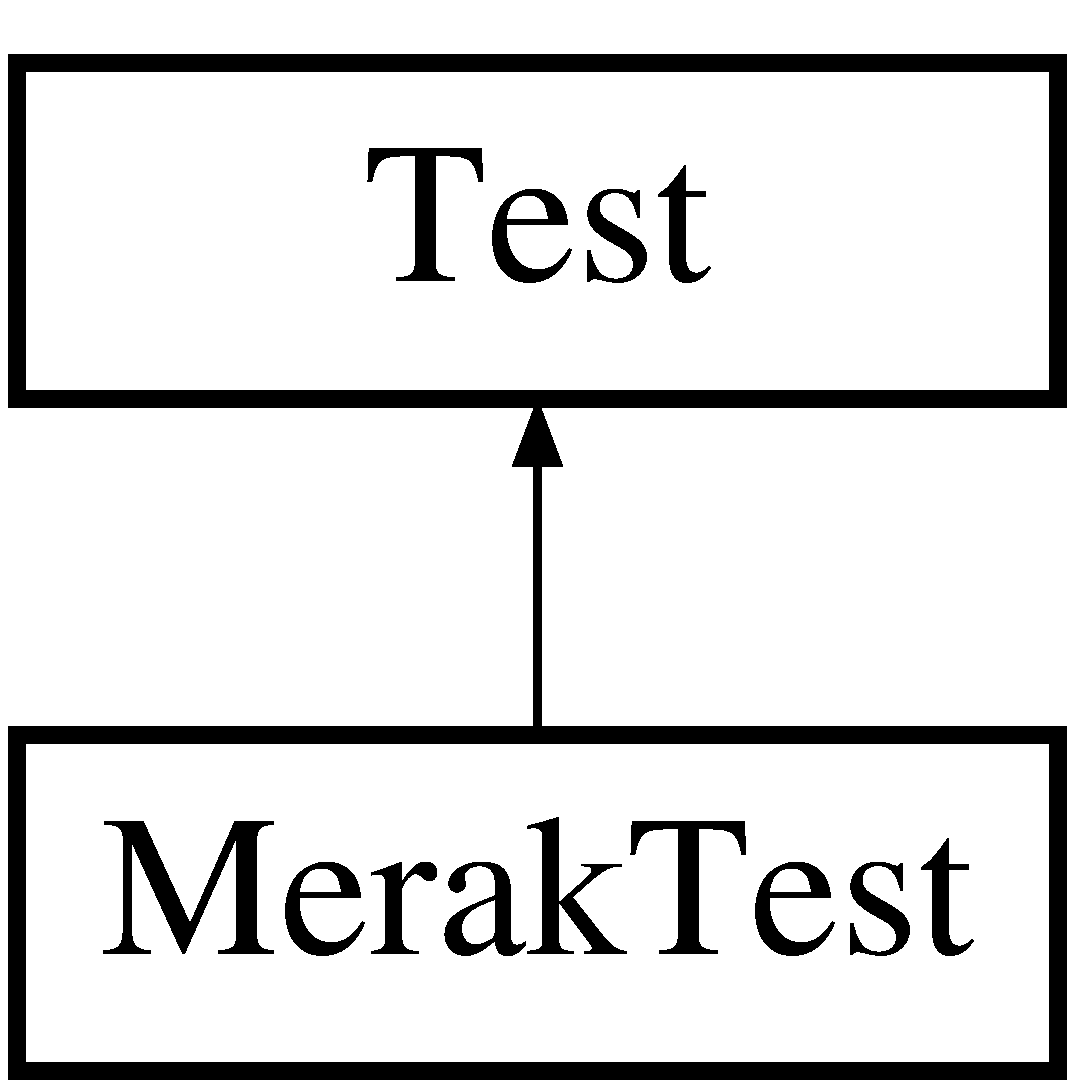
\includegraphics[height=2.000000cm]{class_merak_test}
\end{center}
\end{figure}


The documentation for this class was generated from the following file\+:\begin{DoxyCompactItemize}
\item 
main\+\_\+test.\+cpp\end{DoxyCompactItemize}

\hypertarget{class_panda}{}\section{Panda Class Reference}
\label{class_panda}\index{Panda@{Panda}}
Inheritance diagram for Panda\+:\begin{figure}[H]
\begin{center}
\leavevmode
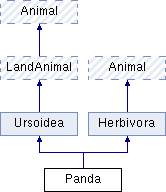
\includegraphics[height=4.000000cm]{class_panda}
\end{center}
\end{figure}
\subsection*{Public Member Functions}
\begin{DoxyCompactItemize}
\item 
\hyperlink{class_panda_a489fdb1f4fe88f0c0c99a3f0768212b4}{Panda} ()\hypertarget{class_panda_a489fdb1f4fe88f0c0c99a3f0768212b4}{}\label{class_panda_a489fdb1f4fe88f0c0c99a3f0768212b4}

\begin{DoxyCompactList}\small\item\em Inisialisasi Hewan. \end{DoxyCompactList}\end{DoxyCompactItemize}
\subsection*{Additional Inherited Members}


The documentation for this class was generated from the following files\+:\begin{DoxyCompactItemize}
\item 
land\+\_\+animal.\+h\item 
land\+\_\+animal.\+cpp\end{DoxyCompactItemize}

\hypertarget{class_panda_test}{}\section{Panda\+Test Class Reference}
\label{class_panda_test}\index{Panda\+Test@{Panda\+Test}}
Inheritance diagram for Panda\+Test\+:\begin{figure}[H]
\begin{center}
\leavevmode
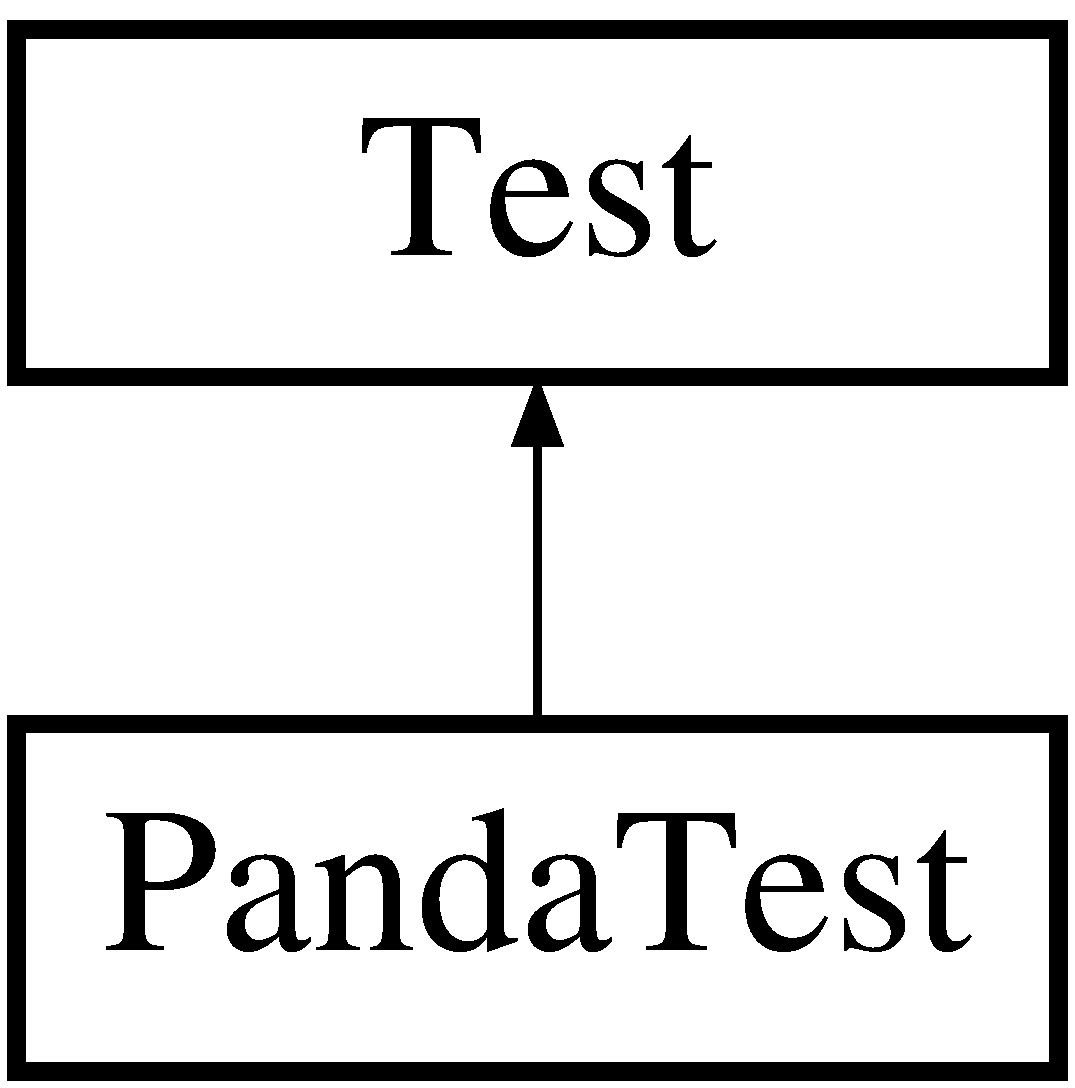
\includegraphics[height=2.000000cm]{class_panda_test}
\end{center}
\end{figure}


The documentation for this class was generated from the following file\+:\begin{DoxyCompactItemize}
\item 
main\+\_\+test.\+cpp\end{DoxyCompactItemize}

\hypertarget{class_pari}{}\section{Pari Class Reference}
\label{class_pari}\index{Pari@{Pari}}
\subsection*{Public Member Functions}
\begin{DoxyCompactItemize}
\item 
\hyperlink{class_pari_a5a119732b193e06037a00456c6606c35}{Pari} ()\hypertarget{class_pari_a5a119732b193e06037a00456c6606c35}{}\label{class_pari_a5a119732b193e06037a00456c6606c35}

\begin{DoxyCompactList}\small\item\em Constructor. \end{DoxyCompactList}\item 
\hyperlink{class_pari_a36087d3c1cef597ddbd54a735377e4cb}{$\sim$\+Pari} ()\hypertarget{class_pari_a36087d3c1cef597ddbd54a735377e4cb}{}\label{class_pari_a36087d3c1cef597ddbd54a735377e4cb}

\begin{DoxyCompactList}\small\item\em Destructor. \end{DoxyCompactList}\item 
string \hyperlink{class_pari_a4dc414c704021fe6bc46c7eaa7d916e7}{Get\+Experience} ()\hypertarget{class_pari_a4dc414c704021fe6bc46c7eaa7d916e7}{}\label{class_pari_a4dc414c704021fe6bc46c7eaa7d916e7}

\begin{DoxyCompactList}\small\item\em Komunikasi dengan hewan. \end{DoxyCompactList}\item 
int \hyperlink{class_pari_abceafaa8a5780e93c62f9d7010cb71e6}{Get\+Food\+Num} ()
\begin{DoxyCompactList}\small\item\em Jumlah makanan. \end{DoxyCompactList}\item 
char \hyperlink{class_pari_a4c4a6399d001827a5f162ef7f61f7adc}{Get\+Render} ()
\begin{DoxyCompactList}\small\item\em Print karakter. \end{DoxyCompactList}\item 
void \hyperlink{class_pari_a75009639d68712191acc97d3e2b085bd}{Set\+Enemy} (char cc)
\begin{DoxyCompactList}\small\item\em Set karakter hewan. \end{DoxyCompactList}\item 
char $\ast$ \hyperlink{class_pari_a0a925b9f16c081d70dd3fb9ed0083f8d}{Get\+Enemy} ()
\begin{DoxyCompactList}\small\item\em Ambil list musuh. \end{DoxyCompactList}\end{DoxyCompactItemize}
\subsection*{Protected Attributes}
\begin{DoxyCompactItemize}
\item 
int $\ast$ \hyperlink{class_pari_a32892923f010b6020f0ce6cb502bd40f}{Type}
\item 
string \hyperlink{class_pari_a04952b36531c2e1e11bc71765ad397ae}{Famili}
\item 
string \hyperlink{class_pari_ae19b6c0ae58cbadd11f5cee76748c08a}{Species}
\item 
string \hyperlink{class_pari_a5af7337a5d81ce05b41684caad72f693}{Experience}
\item 
short \hyperlink{class_pari_a4360fe7222e68c47d0bc708e983c6390}{Jenis\+Makanan}
\item 
int \hyperlink{class_pari_af09ebc3ca43824ed8ad595a5af618b1a}{Berat}
\item 
char \hyperlink{class_pari_adc28998e9196bb80e188140f52990dd4}{Ani\+Char}
\item 
char $\ast$ \hyperlink{class_pari_a9247e9974d727eacf825e3767d79d00d}{Enemy\+Char}
\item 
int \hyperlink{class_pari_a21188e07ff07b057c3898feb81bc8c43}{Top\+Enemy}
\end{DoxyCompactItemize}


\subsection{Member Function Documentation}
\index{Pari@{Pari}!Get\+Enemy@{Get\+Enemy}}
\index{Get\+Enemy@{Get\+Enemy}!Pari@{Pari}}
\subsubsection[{\texorpdfstring{Get\+Enemy()}{GetEnemy()}}]{\setlength{\rightskip}{0pt plus 5cm}char $\ast$ Pari\+::\+Get\+Enemy (
\begin{DoxyParamCaption}
{}
\end{DoxyParamCaption}
)}\hypertarget{class_pari_a0a925b9f16c081d70dd3fb9ed0083f8d}{}\label{class_pari_a0a925b9f16c081d70dd3fb9ed0083f8d}


Ambil list musuh. 

\begin{DoxyReturn}{Returns}
List Musuh 
\end{DoxyReturn}
\index{Pari@{Pari}!Get\+Food\+Num@{Get\+Food\+Num}}
\index{Get\+Food\+Num@{Get\+Food\+Num}!Pari@{Pari}}
\subsubsection[{\texorpdfstring{Get\+Food\+Num()}{GetFoodNum()}}]{\setlength{\rightskip}{0pt plus 5cm}int Pari\+::\+Get\+Food\+Num (
\begin{DoxyParamCaption}
{}
\end{DoxyParamCaption}
)}\hypertarget{class_pari_abceafaa8a5780e93c62f9d7010cb71e6}{}\label{class_pari_abceafaa8a5780e93c62f9d7010cb71e6}


Jumlah makanan. 

\begin{DoxyReturn}{Returns}
Jumlah makan

Jumlah makanan 
\end{DoxyReturn}
\index{Pari@{Pari}!Get\+Render@{Get\+Render}}
\index{Get\+Render@{Get\+Render}!Pari@{Pari}}
\subsubsection[{\texorpdfstring{Get\+Render()}{GetRender()}}]{\setlength{\rightskip}{0pt plus 5cm}char Pari\+::\+Get\+Render (
\begin{DoxyParamCaption}
{}
\end{DoxyParamCaption}
)}\hypertarget{class_pari_a4c4a6399d001827a5f162ef7f61f7adc}{}\label{class_pari_a4c4a6399d001827a5f162ef7f61f7adc}


Print karakter. 

\begin{DoxyReturn}{Returns}
char 
\end{DoxyReturn}
\index{Pari@{Pari}!Set\+Enemy@{Set\+Enemy}}
\index{Set\+Enemy@{Set\+Enemy}!Pari@{Pari}}
\subsubsection[{\texorpdfstring{Set\+Enemy(char cc)}{SetEnemy(char cc)}}]{\setlength{\rightskip}{0pt plus 5cm}void Pari\+::\+Set\+Enemy (
\begin{DoxyParamCaption}
\item[{char}]{cc}
\end{DoxyParamCaption}
)}\hypertarget{class_pari_a75009639d68712191acc97d3e2b085bd}{}\label{class_pari_a75009639d68712191acc97d3e2b085bd}


Set karakter hewan. 


\begin{DoxyParams}{Parameters}
{\em cc} & Karakter hewan tsb \\
\hline
\end{DoxyParams}


\subsection{Member Data Documentation}
\index{Pari@{Pari}!Ani\+Char@{Ani\+Char}}
\index{Ani\+Char@{Ani\+Char}!Pari@{Pari}}
\subsubsection[{\texorpdfstring{Ani\+Char}{AniChar}}]{\setlength{\rightskip}{0pt plus 5cm}char Pari\+::\+Ani\+Char\hspace{0.3cm}{\ttfamily [protected]}}\hypertarget{class_pari_adc28998e9196bb80e188140f52990dd4}{}\label{class_pari_adc28998e9196bb80e188140f52990dd4}
Char yang digunakan untuk render \index{Pari@{Pari}!Berat@{Berat}}
\index{Berat@{Berat}!Pari@{Pari}}
\subsubsection[{\texorpdfstring{Berat}{Berat}}]{\setlength{\rightskip}{0pt plus 5cm}int Pari\+::\+Berat\hspace{0.3cm}{\ttfamily [protected]}}\hypertarget{class_pari_af09ebc3ca43824ed8ad595a5af618b1a}{}\label{class_pari_af09ebc3ca43824ed8ad595a5af618b1a}
Berat hewan \index{Pari@{Pari}!Enemy\+Char@{Enemy\+Char}}
\index{Enemy\+Char@{Enemy\+Char}!Pari@{Pari}}
\subsubsection[{\texorpdfstring{Enemy\+Char}{EnemyChar}}]{\setlength{\rightskip}{0pt plus 5cm}char$\ast$ Pari\+::\+Enemy\+Char\hspace{0.3cm}{\ttfamily [protected]}}\hypertarget{class_pari_a9247e9974d727eacf825e3767d79d00d}{}\label{class_pari_a9247e9974d727eacf825e3767d79d00d}
Array of char yang berisi list musuhnya \index{Pari@{Pari}!Experience@{Experience}}
\index{Experience@{Experience}!Pari@{Pari}}
\subsubsection[{\texorpdfstring{Experience}{Experience}}]{\setlength{\rightskip}{0pt plus 5cm}string Pari\+::\+Experience\hspace{0.3cm}{\ttfamily [protected]}}\hypertarget{class_pari_a5af7337a5d81ce05b41684caad72f693}{}\label{class_pari_a5af7337a5d81ce05b41684caad72f693}
Experience hewan \index{Pari@{Pari}!Famili@{Famili}}
\index{Famili@{Famili}!Pari@{Pari}}
\subsubsection[{\texorpdfstring{Famili}{Famili}}]{\setlength{\rightskip}{0pt plus 5cm}string Pari\+::\+Famili\hspace{0.3cm}{\ttfamily [protected]}}\hypertarget{class_pari_a04952b36531c2e1e11bc71765ad397ae}{}\label{class_pari_a04952b36531c2e1e11bc71765ad397ae}
Family hewan \index{Pari@{Pari}!Jenis\+Makanan@{Jenis\+Makanan}}
\index{Jenis\+Makanan@{Jenis\+Makanan}!Pari@{Pari}}
\subsubsection[{\texorpdfstring{Jenis\+Makanan}{JenisMakanan}}]{\setlength{\rightskip}{0pt plus 5cm}short Pari\+::\+Jenis\+Makanan\hspace{0.3cm}{\ttfamily [protected]}}\hypertarget{class_pari_a4360fe7222e68c47d0bc708e983c6390}{}\label{class_pari_a4360fe7222e68c47d0bc708e983c6390}
Jenis Makanan hewan. 1 \+: herbifor, 2 \+: karnivor, 3 \+: omnifor \index{Pari@{Pari}!Species@{Species}}
\index{Species@{Species}!Pari@{Pari}}
\subsubsection[{\texorpdfstring{Species}{Species}}]{\setlength{\rightskip}{0pt plus 5cm}string Pari\+::\+Species\hspace{0.3cm}{\ttfamily [protected]}}\hypertarget{class_pari_ae19b6c0ae58cbadd11f5cee76748c08a}{}\label{class_pari_ae19b6c0ae58cbadd11f5cee76748c08a}
Species hewan \index{Pari@{Pari}!Top\+Enemy@{Top\+Enemy}}
\index{Top\+Enemy@{Top\+Enemy}!Pari@{Pari}}
\subsubsection[{\texorpdfstring{Top\+Enemy}{TopEnemy}}]{\setlength{\rightskip}{0pt plus 5cm}int Pari\+::\+Top\+Enemy\hspace{0.3cm}{\ttfamily [protected]}}\hypertarget{class_pari_a21188e07ff07b057c3898feb81bc8c43}{}\label{class_pari_a21188e07ff07b057c3898feb81bc8c43}
Pointer Enemy\+Char yang available \index{Pari@{Pari}!Type@{Type}}
\index{Type@{Type}!Pari@{Pari}}
\subsubsection[{\texorpdfstring{Type}{Type}}]{\setlength{\rightskip}{0pt plus 5cm}int$\ast$ Pari\+::\+Type\hspace{0.3cm}{\ttfamily [protected]}}\hypertarget{class_pari_a32892923f010b6020f0ce6cb502bd40f}{}\label{class_pari_a32892923f010b6020f0ce6cb502bd40f}
Type habitat hewan. 0 \+: darat, 1 \+: udara, 2 \+: air 

The documentation for this class was generated from the following files\+:\begin{DoxyCompactItemize}
\item 
pari.\+h\item 
pari.\+cpp\end{DoxyCompactItemize}

\hypertarget{class_pari_test}{}\section{Pari\+Test Class Reference}
\label{class_pari_test}\index{Pari\+Test@{Pari\+Test}}
Inheritance diagram for Pari\+Test\+:\begin{figure}[H]
\begin{center}
\leavevmode
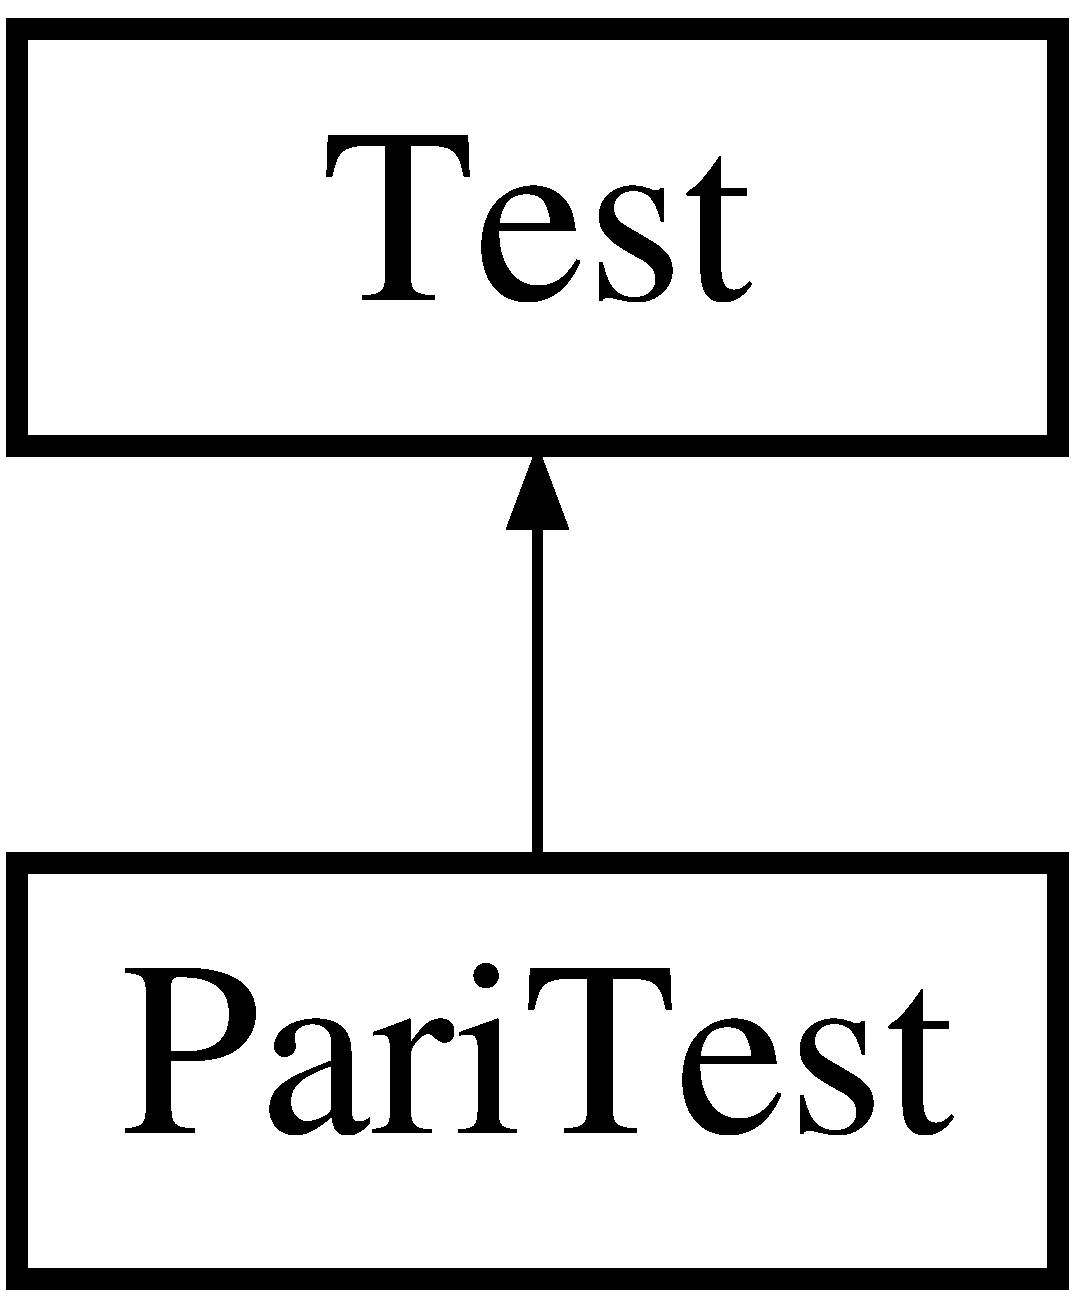
\includegraphics[height=2.000000cm]{class_pari_test}
\end{center}
\end{figure}


The documentation for this class was generated from the following file\+:\begin{DoxyCompactItemize}
\item 
main\+\_\+test.\+cpp\end{DoxyCompactItemize}

\hypertarget{class_penguin}{}\section{Penguin Class Reference}
\label{class_penguin}\index{Penguin@{Penguin}}
Inheritance diagram for Penguin\+:\begin{figure}[H]
\begin{center}
\leavevmode
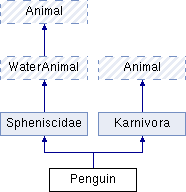
\includegraphics[height=4.000000cm]{class_penguin}
\end{center}
\end{figure}
\subsection*{Public Member Functions}
\begin{DoxyCompactItemize}
\item 
\hyperlink{class_penguin_a215ac88a9d57ac01355e414c0527e862}{Penguin} ()\hypertarget{class_penguin_a215ac88a9d57ac01355e414c0527e862}{}\label{class_penguin_a215ac88a9d57ac01355e414c0527e862}

\begin{DoxyCompactList}\small\item\em Inisialisasi Hewan. \end{DoxyCompactList}\end{DoxyCompactItemize}
\subsection*{Additional Inherited Members}


The documentation for this class was generated from the following files\+:\begin{DoxyCompactItemize}
\item 
water\+\_\+animal.\+h\item 
water\+\_\+animal.\+cpp\end{DoxyCompactItemize}

\hypertarget{class_penguin_test}{}\section{Penguin\+Test Class Reference}
\label{class_penguin_test}\index{Penguin\+Test@{Penguin\+Test}}
Inheritance diagram for Penguin\+Test\+:\begin{figure}[H]
\begin{center}
\leavevmode
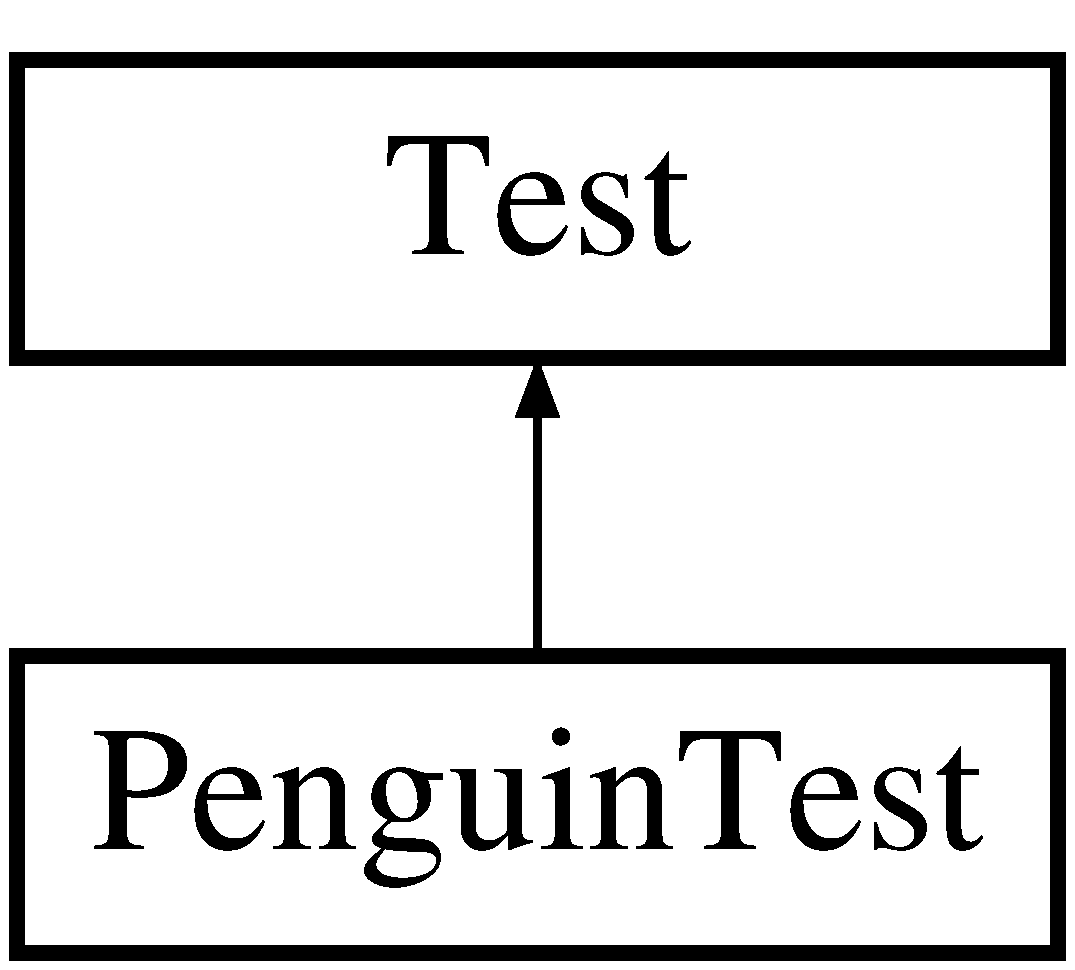
\includegraphics[height=2.000000cm]{class_penguin_test}
\end{center}
\end{figure}


The documentation for this class was generated from the following file\+:\begin{DoxyCompactItemize}
\item 
main\+\_\+test.\+cpp\end{DoxyCompactItemize}

\hypertarget{class_reindeer}{}\section{Reindeer Class Reference}
\label{class_reindeer}\index{Reindeer@{Reindeer}}
\subsection*{Public Member Functions}
\begin{DoxyCompactItemize}
\item 
\hyperlink{class_reindeer_abf6ea0887ccaa39ac9b1d927f4833aaa}{Reindeer} ()\hypertarget{class_reindeer_abf6ea0887ccaa39ac9b1d927f4833aaa}{}\label{class_reindeer_abf6ea0887ccaa39ac9b1d927f4833aaa}

\begin{DoxyCompactList}\small\item\em Constructor. \end{DoxyCompactList}\item 
\hyperlink{class_reindeer_a8459e722edfb7c824d65d24420ad082b}{$\sim$\+Reindeer} ()\hypertarget{class_reindeer_a8459e722edfb7c824d65d24420ad082b}{}\label{class_reindeer_a8459e722edfb7c824d65d24420ad082b}

\begin{DoxyCompactList}\small\item\em Destructor. \end{DoxyCompactList}\item 
string \hyperlink{class_reindeer_a2dc5a553f9ae3af3869c0f7a7f5a5401}{Get\+Experience} ()\hypertarget{class_reindeer_a2dc5a553f9ae3af3869c0f7a7f5a5401}{}\label{class_reindeer_a2dc5a553f9ae3af3869c0f7a7f5a5401}

\begin{DoxyCompactList}\small\item\em Komunikasi dengan hewan. \end{DoxyCompactList}\item 
int \hyperlink{class_reindeer_aae7b2882cbffd078f6420ec6f5ca924d}{Get\+Food\+Num} ()
\begin{DoxyCompactList}\small\item\em Jumlah makanan. \end{DoxyCompactList}\item 
char \hyperlink{class_reindeer_a9e7a92aa2ed70fe9f93d826e63918dea}{Get\+Render} ()
\begin{DoxyCompactList}\small\item\em Print karakter. \end{DoxyCompactList}\item 
void \hyperlink{class_reindeer_a074fa6ffde928eefa7b6c276030c65bc}{Set\+Enemy} (char cc)
\begin{DoxyCompactList}\small\item\em Set karakter hewan. \end{DoxyCompactList}\item 
char $\ast$ \hyperlink{class_reindeer_a94bcac7946ecf20129ee82f2fb713d22}{Get\+Enemy} ()
\begin{DoxyCompactList}\small\item\em Ambil list musuh. \end{DoxyCompactList}\end{DoxyCompactItemize}
\subsection*{Protected Attributes}
\begin{DoxyCompactItemize}
\item 
int $\ast$ \hyperlink{class_reindeer_a58390c66250434a8294b9eac8c204f70}{Type}
\item 
string \hyperlink{class_reindeer_a76954572639868570bb712fa5e9f2416}{Famili}
\item 
string \hyperlink{class_reindeer_a01c318a23a5f18c9a9a854e8f4c5530a}{Species}
\item 
string \hyperlink{class_reindeer_afd7f929fb6835b031d1a8effd2c4fca7}{Experience}
\item 
short \hyperlink{class_reindeer_a22bd8b287b1371169d059c37c4508572}{Jenis\+Makanan}
\item 
int \hyperlink{class_reindeer_a27cffba68365841555697334a54aefe8}{Berat}
\item 
char \hyperlink{class_reindeer_ac7a242c70bb7a11f259c9f407b9292fe}{Ani\+Char}
\item 
char $\ast$ \hyperlink{class_reindeer_a4d6fcc03d3596875e9ff3fe7a4c824fc}{Enemy\+Char}
\item 
int \hyperlink{class_reindeer_a5a17ac5ba35fd3f580dfb5a1cac219f5}{Top\+Enemy}
\end{DoxyCompactItemize}


\subsection{Member Function Documentation}
\index{Reindeer@{Reindeer}!Get\+Enemy@{Get\+Enemy}}
\index{Get\+Enemy@{Get\+Enemy}!Reindeer@{Reindeer}}
\subsubsection[{\texorpdfstring{Get\+Enemy()}{GetEnemy()}}]{\setlength{\rightskip}{0pt plus 5cm}char $\ast$ Reindeer\+::\+Get\+Enemy (
\begin{DoxyParamCaption}
{}
\end{DoxyParamCaption}
)}\hypertarget{class_reindeer_a94bcac7946ecf20129ee82f2fb713d22}{}\label{class_reindeer_a94bcac7946ecf20129ee82f2fb713d22}


Ambil list musuh. 

\begin{DoxyReturn}{Returns}
List Musuh 
\end{DoxyReturn}
\index{Reindeer@{Reindeer}!Get\+Food\+Num@{Get\+Food\+Num}}
\index{Get\+Food\+Num@{Get\+Food\+Num}!Reindeer@{Reindeer}}
\subsubsection[{\texorpdfstring{Get\+Food\+Num()}{GetFoodNum()}}]{\setlength{\rightskip}{0pt plus 5cm}int Reindeer\+::\+Get\+Food\+Num (
\begin{DoxyParamCaption}
{}
\end{DoxyParamCaption}
)}\hypertarget{class_reindeer_aae7b2882cbffd078f6420ec6f5ca924d}{}\label{class_reindeer_aae7b2882cbffd078f6420ec6f5ca924d}


Jumlah makanan. 

\begin{DoxyReturn}{Returns}
Jumlah makan

Jumlah makanan 
\end{DoxyReturn}
\index{Reindeer@{Reindeer}!Get\+Render@{Get\+Render}}
\index{Get\+Render@{Get\+Render}!Reindeer@{Reindeer}}
\subsubsection[{\texorpdfstring{Get\+Render()}{GetRender()}}]{\setlength{\rightskip}{0pt plus 5cm}char Reindeer\+::\+Get\+Render (
\begin{DoxyParamCaption}
{}
\end{DoxyParamCaption}
)}\hypertarget{class_reindeer_a9e7a92aa2ed70fe9f93d826e63918dea}{}\label{class_reindeer_a9e7a92aa2ed70fe9f93d826e63918dea}


Print karakter. 

\begin{DoxyReturn}{Returns}
char 
\end{DoxyReturn}
\index{Reindeer@{Reindeer}!Set\+Enemy@{Set\+Enemy}}
\index{Set\+Enemy@{Set\+Enemy}!Reindeer@{Reindeer}}
\subsubsection[{\texorpdfstring{Set\+Enemy(char cc)}{SetEnemy(char cc)}}]{\setlength{\rightskip}{0pt plus 5cm}void Reindeer\+::\+Set\+Enemy (
\begin{DoxyParamCaption}
\item[{char}]{cc}
\end{DoxyParamCaption}
)}\hypertarget{class_reindeer_a074fa6ffde928eefa7b6c276030c65bc}{}\label{class_reindeer_a074fa6ffde928eefa7b6c276030c65bc}


Set karakter hewan. 


\begin{DoxyParams}{Parameters}
{\em cc} & Karakter hewan tsb \\
\hline
\end{DoxyParams}


\subsection{Member Data Documentation}
\index{Reindeer@{Reindeer}!Ani\+Char@{Ani\+Char}}
\index{Ani\+Char@{Ani\+Char}!Reindeer@{Reindeer}}
\subsubsection[{\texorpdfstring{Ani\+Char}{AniChar}}]{\setlength{\rightskip}{0pt plus 5cm}char Reindeer\+::\+Ani\+Char\hspace{0.3cm}{\ttfamily [protected]}}\hypertarget{class_reindeer_ac7a242c70bb7a11f259c9f407b9292fe}{}\label{class_reindeer_ac7a242c70bb7a11f259c9f407b9292fe}
Char yang digunakan untuk render \index{Reindeer@{Reindeer}!Berat@{Berat}}
\index{Berat@{Berat}!Reindeer@{Reindeer}}
\subsubsection[{\texorpdfstring{Berat}{Berat}}]{\setlength{\rightskip}{0pt plus 5cm}int Reindeer\+::\+Berat\hspace{0.3cm}{\ttfamily [protected]}}\hypertarget{class_reindeer_a27cffba68365841555697334a54aefe8}{}\label{class_reindeer_a27cffba68365841555697334a54aefe8}
Berat hewan \index{Reindeer@{Reindeer}!Enemy\+Char@{Enemy\+Char}}
\index{Enemy\+Char@{Enemy\+Char}!Reindeer@{Reindeer}}
\subsubsection[{\texorpdfstring{Enemy\+Char}{EnemyChar}}]{\setlength{\rightskip}{0pt plus 5cm}char$\ast$ Reindeer\+::\+Enemy\+Char\hspace{0.3cm}{\ttfamily [protected]}}\hypertarget{class_reindeer_a4d6fcc03d3596875e9ff3fe7a4c824fc}{}\label{class_reindeer_a4d6fcc03d3596875e9ff3fe7a4c824fc}
Array of char yang berisi list musuhnya \index{Reindeer@{Reindeer}!Experience@{Experience}}
\index{Experience@{Experience}!Reindeer@{Reindeer}}
\subsubsection[{\texorpdfstring{Experience}{Experience}}]{\setlength{\rightskip}{0pt plus 5cm}string Reindeer\+::\+Experience\hspace{0.3cm}{\ttfamily [protected]}}\hypertarget{class_reindeer_afd7f929fb6835b031d1a8effd2c4fca7}{}\label{class_reindeer_afd7f929fb6835b031d1a8effd2c4fca7}
Experience hewan \index{Reindeer@{Reindeer}!Famili@{Famili}}
\index{Famili@{Famili}!Reindeer@{Reindeer}}
\subsubsection[{\texorpdfstring{Famili}{Famili}}]{\setlength{\rightskip}{0pt plus 5cm}string Reindeer\+::\+Famili\hspace{0.3cm}{\ttfamily [protected]}}\hypertarget{class_reindeer_a76954572639868570bb712fa5e9f2416}{}\label{class_reindeer_a76954572639868570bb712fa5e9f2416}
Family hewan \index{Reindeer@{Reindeer}!Jenis\+Makanan@{Jenis\+Makanan}}
\index{Jenis\+Makanan@{Jenis\+Makanan}!Reindeer@{Reindeer}}
\subsubsection[{\texorpdfstring{Jenis\+Makanan}{JenisMakanan}}]{\setlength{\rightskip}{0pt plus 5cm}short Reindeer\+::\+Jenis\+Makanan\hspace{0.3cm}{\ttfamily [protected]}}\hypertarget{class_reindeer_a22bd8b287b1371169d059c37c4508572}{}\label{class_reindeer_a22bd8b287b1371169d059c37c4508572}
Jenis Makanan hewan. 1 \+: herbifor, 2 \+: karnivor, 3 \+: omnifor \index{Reindeer@{Reindeer}!Species@{Species}}
\index{Species@{Species}!Reindeer@{Reindeer}}
\subsubsection[{\texorpdfstring{Species}{Species}}]{\setlength{\rightskip}{0pt plus 5cm}string Reindeer\+::\+Species\hspace{0.3cm}{\ttfamily [protected]}}\hypertarget{class_reindeer_a01c318a23a5f18c9a9a854e8f4c5530a}{}\label{class_reindeer_a01c318a23a5f18c9a9a854e8f4c5530a}
Species hewan \index{Reindeer@{Reindeer}!Top\+Enemy@{Top\+Enemy}}
\index{Top\+Enemy@{Top\+Enemy}!Reindeer@{Reindeer}}
\subsubsection[{\texorpdfstring{Top\+Enemy}{TopEnemy}}]{\setlength{\rightskip}{0pt plus 5cm}int Reindeer\+::\+Top\+Enemy\hspace{0.3cm}{\ttfamily [protected]}}\hypertarget{class_reindeer_a5a17ac5ba35fd3f580dfb5a1cac219f5}{}\label{class_reindeer_a5a17ac5ba35fd3f580dfb5a1cac219f5}
Pointer Enemy\+Char yang available \index{Reindeer@{Reindeer}!Type@{Type}}
\index{Type@{Type}!Reindeer@{Reindeer}}
\subsubsection[{\texorpdfstring{Type}{Type}}]{\setlength{\rightskip}{0pt plus 5cm}int$\ast$ Reindeer\+::\+Type\hspace{0.3cm}{\ttfamily [protected]}}\hypertarget{class_reindeer_a58390c66250434a8294b9eac8c204f70}{}\label{class_reindeer_a58390c66250434a8294b9eac8c204f70}
Type habitat hewan. 0 \+: darat, 1 \+: udara, 2 \+: air 

The documentation for this class was generated from the following files\+:\begin{DoxyCompactItemize}
\item 
reindeer.\+h\item 
reindeer.\+cpp\end{DoxyCompactItemize}

\hypertarget{class_reindeer_test}{}\section{Reindeer\+Test Class Reference}
\label{class_reindeer_test}\index{Reindeer\+Test@{Reindeer\+Test}}
Inheritance diagram for Reindeer\+Test\+:\begin{figure}[H]
\begin{center}
\leavevmode
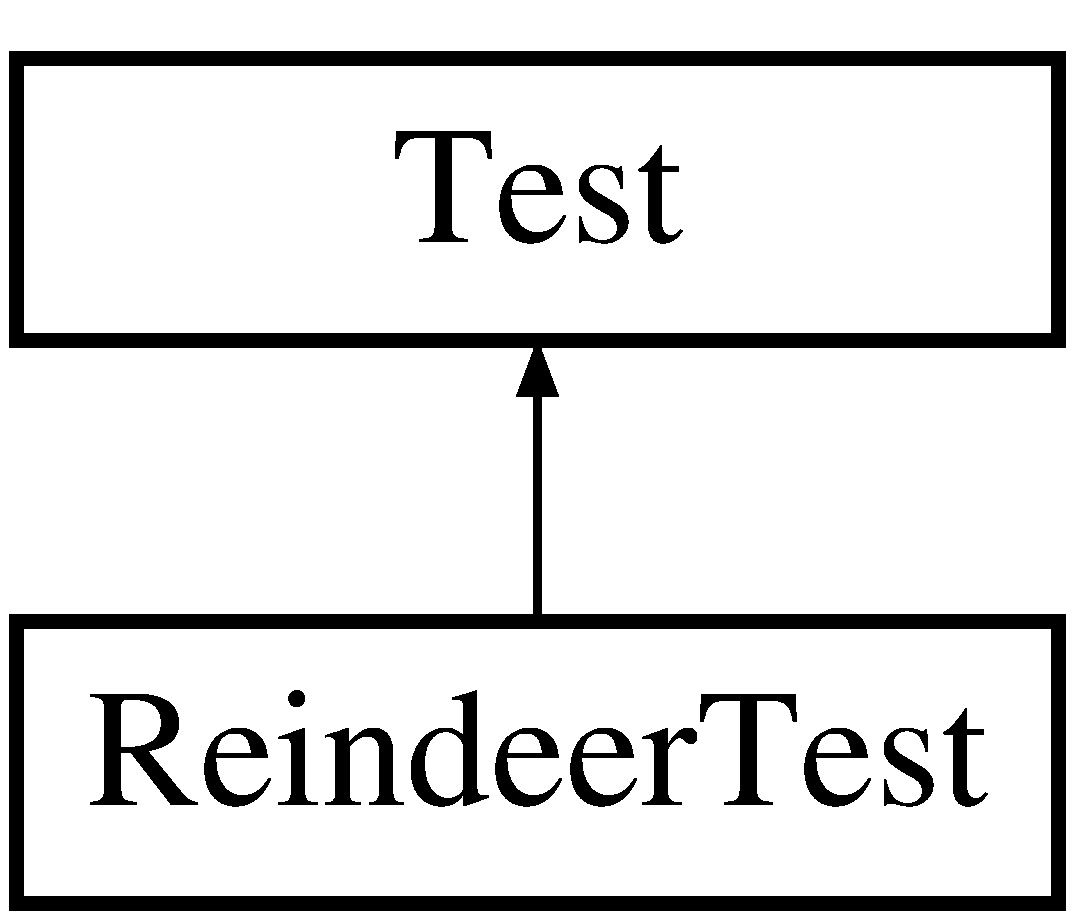
\includegraphics[height=2.000000cm]{class_reindeer_test}
\end{center}
\end{figure}


The documentation for this class was generated from the following file\+:\begin{DoxyCompactItemize}
\item 
main\+\_\+test.\+cpp\end{DoxyCompactItemize}

\hypertarget{class_rhino}{}\section{Rhino Class Reference}
\label{class_rhino}\index{Rhino@{Rhino}}
\subsection*{Public Member Functions}
\begin{DoxyCompactItemize}
\item 
\hyperlink{class_rhino_aa2db135ac8e800310f0531cdbe18bafe}{Rhino} ()\hypertarget{class_rhino_aa2db135ac8e800310f0531cdbe18bafe}{}\label{class_rhino_aa2db135ac8e800310f0531cdbe18bafe}

\begin{DoxyCompactList}\small\item\em Inisialisasi Hewan. \end{DoxyCompactList}\item 
\hyperlink{class_rhino_a6a11f0f8dcd6ed20ef99d8d698b06f28}{$\sim$\+Rhino} ()\hypertarget{class_rhino_a6a11f0f8dcd6ed20ef99d8d698b06f28}{}\label{class_rhino_a6a11f0f8dcd6ed20ef99d8d698b06f28}

\begin{DoxyCompactList}\small\item\em Destructor. \end{DoxyCompactList}\item 
string \hyperlink{class_rhino_a74c81cc9af2162e2c6815059bacf402d}{Get\+Experience} ()\hypertarget{class_rhino_a74c81cc9af2162e2c6815059bacf402d}{}\label{class_rhino_a74c81cc9af2162e2c6815059bacf402d}

\begin{DoxyCompactList}\small\item\em Komunikasi dengan hewan. \end{DoxyCompactList}\item 
int \hyperlink{class_rhino_a3a31a388e2f43865267cbc6f025fd5da}{Get\+Food\+Num} ()
\begin{DoxyCompactList}\small\item\em Jumlah makanan. \end{DoxyCompactList}\item 
char \hyperlink{class_rhino_a8b6eb9e8e19af712e93fcf192afc30b9}{Get\+Render} ()
\begin{DoxyCompactList}\small\item\em Print karakter. \end{DoxyCompactList}\item 
void \hyperlink{class_rhino_a7a19b29742ac6fdddf93142d2c2a838d}{Set\+Enemy} (char cc)
\begin{DoxyCompactList}\small\item\em Set karakter hewan. \end{DoxyCompactList}\item 
char $\ast$ \hyperlink{class_rhino_ac45bb151e13f6ec3df84ab25eb2af5d9}{Get\+Enemy} ()
\begin{DoxyCompactList}\small\item\em Ambil list musuh. \end{DoxyCompactList}\end{DoxyCompactItemize}
\subsection*{Protected Attributes}
\begin{DoxyCompactItemize}
\item 
int $\ast$ \hyperlink{class_rhino_ae1ab730d941b1f359e0b85a66055fcec}{Type}
\item 
string \hyperlink{class_rhino_a2c816e41f908b29a368b3c76e5ad64df}{Famili}
\item 
string \hyperlink{class_rhino_a8e0375e6d689c63aa136c0eaa818f0a4}{Species}
\item 
string \hyperlink{class_rhino_ad94f8ff397bf71bcc2904d45e8867ebc}{Experience}
\item 
short \hyperlink{class_rhino_aea38cb61238b4165de624eb31e9116f4}{Jenis\+Makanan}
\item 
int \hyperlink{class_rhino_ac06d9f600a60ae1dfe379f180628108e}{Berat}
\item 
char \hyperlink{class_rhino_a2784afe60a873a82ab7b8589879ef0da}{Ani\+Char}
\item 
char $\ast$ \hyperlink{class_rhino_a7d5163bf655c96d96a5ac470123ebdbf}{Enemy\+Char}
\item 
int \hyperlink{class_rhino_a68e7c24e66e2fee5a812847616dac9c8}{Top\+Enemy}
\end{DoxyCompactItemize}


\subsection{Member Function Documentation}
\index{Rhino@{Rhino}!Get\+Enemy@{Get\+Enemy}}
\index{Get\+Enemy@{Get\+Enemy}!Rhino@{Rhino}}
\subsubsection[{\texorpdfstring{Get\+Enemy()}{GetEnemy()}}]{\setlength{\rightskip}{0pt plus 5cm}char $\ast$ Rhino\+::\+Get\+Enemy (
\begin{DoxyParamCaption}
{}
\end{DoxyParamCaption}
)}\hypertarget{class_rhino_ac45bb151e13f6ec3df84ab25eb2af5d9}{}\label{class_rhino_ac45bb151e13f6ec3df84ab25eb2af5d9}


Ambil list musuh. 

\begin{DoxyReturn}{Returns}
List Musuh 
\end{DoxyReturn}
\index{Rhino@{Rhino}!Get\+Food\+Num@{Get\+Food\+Num}}
\index{Get\+Food\+Num@{Get\+Food\+Num}!Rhino@{Rhino}}
\subsubsection[{\texorpdfstring{Get\+Food\+Num()}{GetFoodNum()}}]{\setlength{\rightskip}{0pt plus 5cm}int Rhino\+::\+Get\+Food\+Num (
\begin{DoxyParamCaption}
{}
\end{DoxyParamCaption}
)}\hypertarget{class_rhino_a3a31a388e2f43865267cbc6f025fd5da}{}\label{class_rhino_a3a31a388e2f43865267cbc6f025fd5da}


Jumlah makanan. 

\begin{DoxyReturn}{Returns}
Jumlah makan

Jumlah makanan 
\end{DoxyReturn}
\index{Rhino@{Rhino}!Get\+Render@{Get\+Render}}
\index{Get\+Render@{Get\+Render}!Rhino@{Rhino}}
\subsubsection[{\texorpdfstring{Get\+Render()}{GetRender()}}]{\setlength{\rightskip}{0pt plus 5cm}char Rhino\+::\+Get\+Render (
\begin{DoxyParamCaption}
{}
\end{DoxyParamCaption}
)}\hypertarget{class_rhino_a8b6eb9e8e19af712e93fcf192afc30b9}{}\label{class_rhino_a8b6eb9e8e19af712e93fcf192afc30b9}


Print karakter. 

\begin{DoxyReturn}{Returns}
char 
\end{DoxyReturn}
\index{Rhino@{Rhino}!Set\+Enemy@{Set\+Enemy}}
\index{Set\+Enemy@{Set\+Enemy}!Rhino@{Rhino}}
\subsubsection[{\texorpdfstring{Set\+Enemy(char cc)}{SetEnemy(char cc)}}]{\setlength{\rightskip}{0pt plus 5cm}void Rhino\+::\+Set\+Enemy (
\begin{DoxyParamCaption}
\item[{char}]{cc}
\end{DoxyParamCaption}
)}\hypertarget{class_rhino_a7a19b29742ac6fdddf93142d2c2a838d}{}\label{class_rhino_a7a19b29742ac6fdddf93142d2c2a838d}


Set karakter hewan. 


\begin{DoxyParams}{Parameters}
{\em cc} & Karakter hewan tsb \\
\hline
\end{DoxyParams}


\subsection{Member Data Documentation}
\index{Rhino@{Rhino}!Ani\+Char@{Ani\+Char}}
\index{Ani\+Char@{Ani\+Char}!Rhino@{Rhino}}
\subsubsection[{\texorpdfstring{Ani\+Char}{AniChar}}]{\setlength{\rightskip}{0pt plus 5cm}char Rhino\+::\+Ani\+Char\hspace{0.3cm}{\ttfamily [protected]}}\hypertarget{class_rhino_a2784afe60a873a82ab7b8589879ef0da}{}\label{class_rhino_a2784afe60a873a82ab7b8589879ef0da}
Char yang digunakan untuk render \index{Rhino@{Rhino}!Berat@{Berat}}
\index{Berat@{Berat}!Rhino@{Rhino}}
\subsubsection[{\texorpdfstring{Berat}{Berat}}]{\setlength{\rightskip}{0pt plus 5cm}int Rhino\+::\+Berat\hspace{0.3cm}{\ttfamily [protected]}}\hypertarget{class_rhino_ac06d9f600a60ae1dfe379f180628108e}{}\label{class_rhino_ac06d9f600a60ae1dfe379f180628108e}
Berat hewan \index{Rhino@{Rhino}!Enemy\+Char@{Enemy\+Char}}
\index{Enemy\+Char@{Enemy\+Char}!Rhino@{Rhino}}
\subsubsection[{\texorpdfstring{Enemy\+Char}{EnemyChar}}]{\setlength{\rightskip}{0pt plus 5cm}char$\ast$ Rhino\+::\+Enemy\+Char\hspace{0.3cm}{\ttfamily [protected]}}\hypertarget{class_rhino_a7d5163bf655c96d96a5ac470123ebdbf}{}\label{class_rhino_a7d5163bf655c96d96a5ac470123ebdbf}
Array of char yang berisi list musuhnya \index{Rhino@{Rhino}!Experience@{Experience}}
\index{Experience@{Experience}!Rhino@{Rhino}}
\subsubsection[{\texorpdfstring{Experience}{Experience}}]{\setlength{\rightskip}{0pt plus 5cm}string Rhino\+::\+Experience\hspace{0.3cm}{\ttfamily [protected]}}\hypertarget{class_rhino_ad94f8ff397bf71bcc2904d45e8867ebc}{}\label{class_rhino_ad94f8ff397bf71bcc2904d45e8867ebc}
Experience hewan \index{Rhino@{Rhino}!Famili@{Famili}}
\index{Famili@{Famili}!Rhino@{Rhino}}
\subsubsection[{\texorpdfstring{Famili}{Famili}}]{\setlength{\rightskip}{0pt plus 5cm}string Rhino\+::\+Famili\hspace{0.3cm}{\ttfamily [protected]}}\hypertarget{class_rhino_a2c816e41f908b29a368b3c76e5ad64df}{}\label{class_rhino_a2c816e41f908b29a368b3c76e5ad64df}
Family hewan \index{Rhino@{Rhino}!Jenis\+Makanan@{Jenis\+Makanan}}
\index{Jenis\+Makanan@{Jenis\+Makanan}!Rhino@{Rhino}}
\subsubsection[{\texorpdfstring{Jenis\+Makanan}{JenisMakanan}}]{\setlength{\rightskip}{0pt plus 5cm}short Rhino\+::\+Jenis\+Makanan\hspace{0.3cm}{\ttfamily [protected]}}\hypertarget{class_rhino_aea38cb61238b4165de624eb31e9116f4}{}\label{class_rhino_aea38cb61238b4165de624eb31e9116f4}
Jenis Makanan hewan. 1 \+: herbifor, 2 \+: karnivor, 3 \+: omnifor \index{Rhino@{Rhino}!Species@{Species}}
\index{Species@{Species}!Rhino@{Rhino}}
\subsubsection[{\texorpdfstring{Species}{Species}}]{\setlength{\rightskip}{0pt plus 5cm}string Rhino\+::\+Species\hspace{0.3cm}{\ttfamily [protected]}}\hypertarget{class_rhino_a8e0375e6d689c63aa136c0eaa818f0a4}{}\label{class_rhino_a8e0375e6d689c63aa136c0eaa818f0a4}
Species hewan \index{Rhino@{Rhino}!Top\+Enemy@{Top\+Enemy}}
\index{Top\+Enemy@{Top\+Enemy}!Rhino@{Rhino}}
\subsubsection[{\texorpdfstring{Top\+Enemy}{TopEnemy}}]{\setlength{\rightskip}{0pt plus 5cm}int Rhino\+::\+Top\+Enemy\hspace{0.3cm}{\ttfamily [protected]}}\hypertarget{class_rhino_a68e7c24e66e2fee5a812847616dac9c8}{}\label{class_rhino_a68e7c24e66e2fee5a812847616dac9c8}
Pointer Enemy\+Char yang available \index{Rhino@{Rhino}!Type@{Type}}
\index{Type@{Type}!Rhino@{Rhino}}
\subsubsection[{\texorpdfstring{Type}{Type}}]{\setlength{\rightskip}{0pt plus 5cm}int$\ast$ Rhino\+::\+Type\hspace{0.3cm}{\ttfamily [protected]}}\hypertarget{class_rhino_ae1ab730d941b1f359e0b85a66055fcec}{}\label{class_rhino_ae1ab730d941b1f359e0b85a66055fcec}
Type habitat hewan. 0 \+: darat, 1 \+: udara, 2 \+: air 

The documentation for this class was generated from the following files\+:\begin{DoxyCompactItemize}
\item 
rhino.\+h\item 
rhino.\+cpp\end{DoxyCompactItemize}

\hypertarget{class_rhino_test}{}\section{Rhino\+Test Class Reference}
\label{class_rhino_test}\index{Rhino\+Test@{Rhino\+Test}}
Inheritance diagram for Rhino\+Test\+:\begin{figure}[H]
\begin{center}
\leavevmode
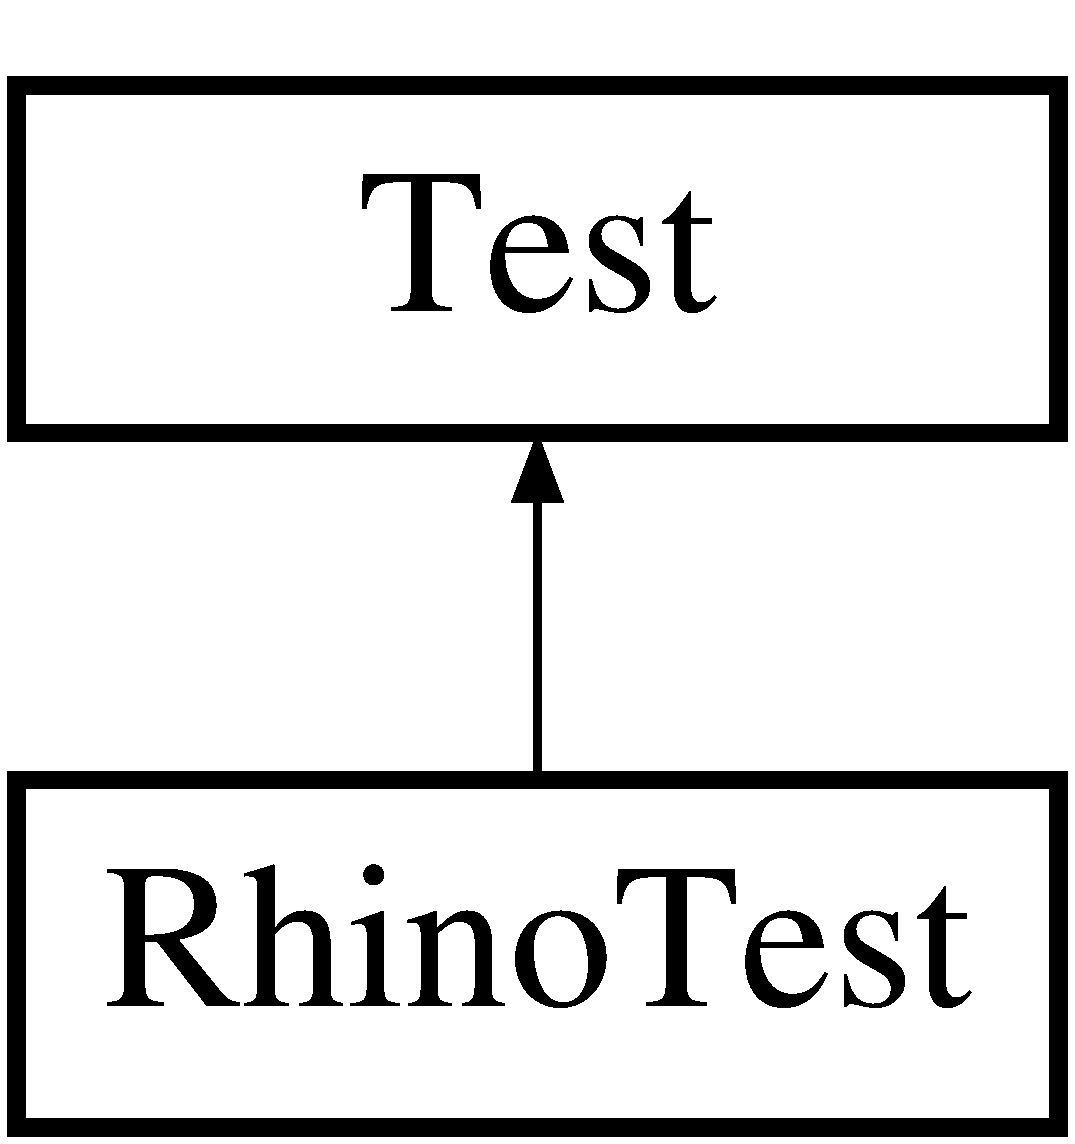
\includegraphics[height=2.000000cm]{class_rhino_test}
\end{center}
\end{figure}


The documentation for this class was generated from the following file\+:\begin{DoxyCompactItemize}
\item 
main\+\_\+test.\+cpp\end{DoxyCompactItemize}

\hypertarget{class_road}{}\section{Road Class Reference}
\label{class_road}\index{Road@{Road}}
Inheritance diagram for Road\+:\begin{figure}[H]
\begin{center}
\leavevmode
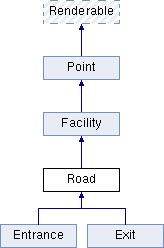
\includegraphics[height=5.000000cm]{class_road}
\end{center}
\end{figure}
\subsection*{Public Member Functions}
\begin{DoxyCompactItemize}
\item 
\hyperlink{class_road_a667617723b2471143dac5dacf97fe8d8}{Road} (int pos\+\_\+x, int pos\+\_\+y)
\begin{DoxyCompactList}\small\item\em jalan \end{DoxyCompactList}\item 
virtual bool \hyperlink{class_road_a0363fc19374b8fa525ee66a3eb255258}{Is\+Jalan} ()
\begin{DoxyCompactList}\small\item\em Is\+Jalan. \end{DoxyCompactList}\item 
char \hyperlink{class_road_ad280899c91650d6f0968c54680db74d6}{Render} ()
\begin{DoxyCompactList}\small\item\em Kelas virtual render. \end{DoxyCompactList}\end{DoxyCompactItemize}
\subsection*{Additional Inherited Members}


\subsection{Constructor \& Destructor Documentation}
\index{Road@{Road}!Road@{Road}}
\index{Road@{Road}!Road@{Road}}
\subsubsection[{\texorpdfstring{Road(int pos\+\_\+x, int pos\+\_\+y)}{Road(int pos_x, int pos_y)}}]{\setlength{\rightskip}{0pt plus 5cm}Road\+::\+Road (
\begin{DoxyParamCaption}
\item[{int}]{pos\+\_\+x, }
\item[{int}]{pos\+\_\+y}
\end{DoxyParamCaption}
)}\hypertarget{class_road_a667617723b2471143dac5dacf97fe8d8}{}\label{class_road_a667617723b2471143dac5dacf97fe8d8}


jalan 


\begin{DoxyParams}{Parameters}
{\em pos\+\_\+x} & posisi x \\
\hline
{\em pos\+\_\+y} & posisi y \\
\hline
\end{DoxyParams}


\subsection{Member Function Documentation}
\index{Road@{Road}!Is\+Jalan@{Is\+Jalan}}
\index{Is\+Jalan@{Is\+Jalan}!Road@{Road}}
\subsubsection[{\texorpdfstring{Is\+Jalan()}{IsJalan()}}]{\setlength{\rightskip}{0pt plus 5cm}bool Road\+::\+Is\+Jalan (
\begin{DoxyParamCaption}
{}
\end{DoxyParamCaption}
)\hspace{0.3cm}{\ttfamily [virtual]}}\hypertarget{class_road_a0363fc19374b8fa525ee66a3eb255258}{}\label{class_road_a0363fc19374b8fa525ee66a3eb255258}


Is\+Jalan. 

\begin{DoxyReturn}{Returns}
true jika jalan. 
\end{DoxyReturn}


Reimplemented from \hyperlink{class_point_a09d84d2aa58ff1257e4c08ff472c6530}{Point}.

\index{Road@{Road}!Render@{Render}}
\index{Render@{Render}!Road@{Road}}
\subsubsection[{\texorpdfstring{Render()}{Render()}}]{\setlength{\rightskip}{0pt plus 5cm}char Road\+::\+Render (
\begin{DoxyParamCaption}
{}
\end{DoxyParamCaption}
)\hspace{0.3cm}{\ttfamily [virtual]}}\hypertarget{class_road_ad280899c91650d6f0968c54680db74d6}{}\label{class_road_ad280899c91650d6f0968c54680db74d6}


Kelas virtual render. 


\begin{DoxyParams}{Parameters}
{\em cc} & matriks yang akan diprint \\
\hline
\end{DoxyParams}


Reimplemented from \hyperlink{class_renderable_aee3f28b28858ab23039ba8416ff93ec2}{Renderable}.



The documentation for this class was generated from the following files\+:\begin{DoxyCompactItemize}
\item 
road.\+h\item 
road.\+cpp\end{DoxyCompactItemize}

\hypertarget{class_road_test}{}\section{Road\+Test Class Reference}
\label{class_road_test}\index{Road\+Test@{Road\+Test}}
Inheritance diagram for Road\+Test\+:\begin{figure}[H]
\begin{center}
\leavevmode
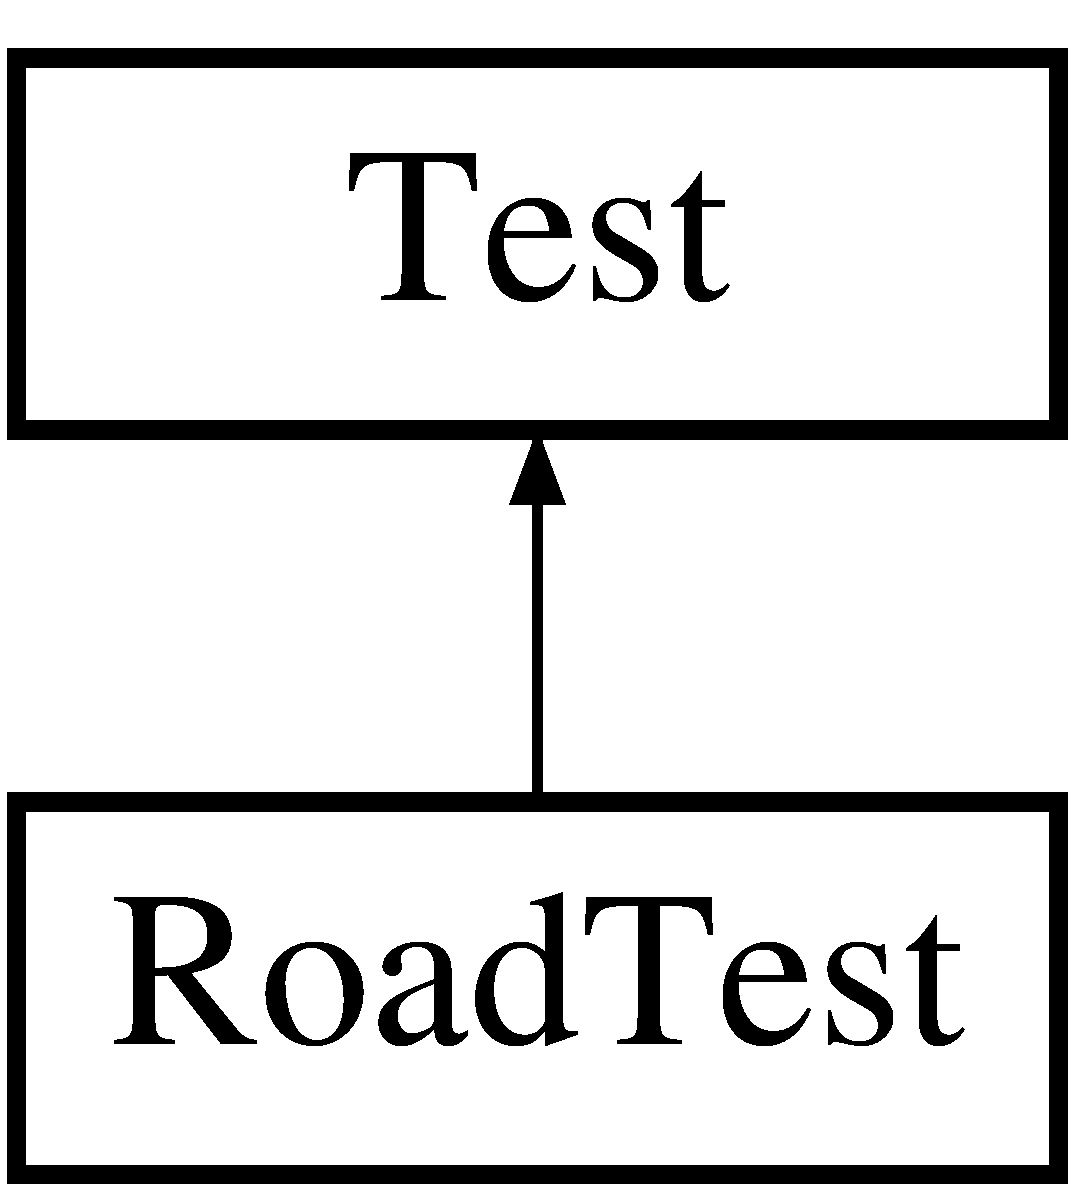
\includegraphics[height=2.000000cm]{class_road_test}
\end{center}
\end{figure}


The documentation for this class was generated from the following file\+:\begin{DoxyCompactItemize}
\item 
main\+\_\+test.\+cpp\end{DoxyCompactItemize}

\hypertarget{class_sample}{}\section{Sample Class Reference}
\label{class_sample}\index{Sample@{Sample}}
\subsection*{Public Member Functions}
\begin{DoxyCompactItemize}
\item 
void {\bfseries Add} (int x)\hypertarget{class_sample_aaef14f95b2f52d048de8b0f43519fe35}{}\label{class_sample_aaef14f95b2f52d048de8b0f43519fe35}

\item 
void {\bfseries Min} (int x)\hypertarget{class_sample_ac2f36c7cea143a69151f5db38b8337e9}{}\label{class_sample_ac2f36c7cea143a69151f5db38b8337e9}

\item 
void {\bfseries Print} ()\hypertarget{class_sample_a4fb8a2e8d124ae41c13e7e5abb3dce08}{}\label{class_sample_a4fb8a2e8d124ae41c13e7e5abb3dce08}

\item 
int {\bfseries get\+Val} ()\hypertarget{class_sample_ab25087ebc51588d3cabe557ef516d4d9}{}\label{class_sample_ab25087ebc51588d3cabe557ef516d4d9}

\end{DoxyCompactItemize}


The documentation for this class was generated from the following files\+:\begin{DoxyCompactItemize}
\item 
sample.\+h\item 
sample.\+cpp\end{DoxyCompactItemize}

\hypertarget{class_sea_dragon}{}\section{Sea\+Dragon Class Reference}
\label{class_sea_dragon}\index{Sea\+Dragon@{Sea\+Dragon}}
\subsection*{Public Member Functions}
\begin{DoxyCompactItemize}
\item 
\hyperlink{class_sea_dragon_a87c431ca8f3a6449abac5a55df87349b}{Sea\+Dragon} ()\hypertarget{class_sea_dragon_a87c431ca8f3a6449abac5a55df87349b}{}\label{class_sea_dragon_a87c431ca8f3a6449abac5a55df87349b}

\begin{DoxyCompactList}\small\item\em Constructor. \end{DoxyCompactList}\item 
\hyperlink{class_sea_dragon_a32875e956b9d03aff59005f90dcd7869}{$\sim$\+Sea\+Dragon} ()\hypertarget{class_sea_dragon_a32875e956b9d03aff59005f90dcd7869}{}\label{class_sea_dragon_a32875e956b9d03aff59005f90dcd7869}

\begin{DoxyCompactList}\small\item\em Destructor. \end{DoxyCompactList}\item 
string \hyperlink{class_sea_dragon_a0c65956887dc12ef009ed25821f8f4a8}{Get\+Experience} ()\hypertarget{class_sea_dragon_a0c65956887dc12ef009ed25821f8f4a8}{}\label{class_sea_dragon_a0c65956887dc12ef009ed25821f8f4a8}

\begin{DoxyCompactList}\small\item\em Komunikasi dengan hewan. \end{DoxyCompactList}\item 
int \hyperlink{class_sea_dragon_abef8ebb7593ca99a79bf5460de84194f}{Get\+Food\+Num} ()
\begin{DoxyCompactList}\small\item\em Jumlah makanan. \end{DoxyCompactList}\item 
char \hyperlink{class_sea_dragon_a524a79b35a2d9ae060edb2378c3e622a}{Get\+Render} ()
\begin{DoxyCompactList}\small\item\em Print karakter. \end{DoxyCompactList}\item 
void \hyperlink{class_sea_dragon_af3f0afbb67cc6c52646f02c82c265c89}{Set\+Enemy} (char cc)
\begin{DoxyCompactList}\small\item\em Set karakter hewan. \end{DoxyCompactList}\item 
char $\ast$ \hyperlink{class_sea_dragon_a51b8efd7a8a0fc47e2b3df0b4d8b8abd}{Get\+Enemy} ()
\begin{DoxyCompactList}\small\item\em Ambil list musuh. \end{DoxyCompactList}\end{DoxyCompactItemize}
\subsection*{Protected Attributes}
\begin{DoxyCompactItemize}
\item 
int $\ast$ \hyperlink{class_sea_dragon_a637d2f83f9e3ac2a24c981dd7fc6313b}{Type}
\item 
string \hyperlink{class_sea_dragon_a40ff623ba2816d34c630569da6c13bcd}{Famili}
\item 
string \hyperlink{class_sea_dragon_a7f5f1a4022a09dbfed539a25ed2aba17}{Species}
\item 
string \hyperlink{class_sea_dragon_a6e46d2d7a8807dfd4020a71699cae2ae}{Experience}
\item 
short \hyperlink{class_sea_dragon_ac834a54d7353af6282c1842b8ea411e7}{Jenis\+Makanan}
\item 
int \hyperlink{class_sea_dragon_a1cc4f1dc2b2f02045e4ad060cc754744}{Berat}
\item 
char \hyperlink{class_sea_dragon_aad356a8af44231e1bbde40567f0af7c1}{Ani\+Char}
\item 
char $\ast$ \hyperlink{class_sea_dragon_a0f81865d76a2f786aa0d095caf2c1607}{Enemy\+Char}
\item 
int \hyperlink{class_sea_dragon_a0848b59807364d124c40d0d4b344d22e}{Top\+Enemy}
\end{DoxyCompactItemize}


\subsection{Member Function Documentation}
\index{Sea\+Dragon@{Sea\+Dragon}!Get\+Enemy@{Get\+Enemy}}
\index{Get\+Enemy@{Get\+Enemy}!Sea\+Dragon@{Sea\+Dragon}}
\subsubsection[{\texorpdfstring{Get\+Enemy()}{GetEnemy()}}]{\setlength{\rightskip}{0pt plus 5cm}char $\ast$ Sea\+Dragon\+::\+Get\+Enemy (
\begin{DoxyParamCaption}
{}
\end{DoxyParamCaption}
)}\hypertarget{class_sea_dragon_a51b8efd7a8a0fc47e2b3df0b4d8b8abd}{}\label{class_sea_dragon_a51b8efd7a8a0fc47e2b3df0b4d8b8abd}


Ambil list musuh. 

\begin{DoxyReturn}{Returns}
List Musuh 
\end{DoxyReturn}
\index{Sea\+Dragon@{Sea\+Dragon}!Get\+Food\+Num@{Get\+Food\+Num}}
\index{Get\+Food\+Num@{Get\+Food\+Num}!Sea\+Dragon@{Sea\+Dragon}}
\subsubsection[{\texorpdfstring{Get\+Food\+Num()}{GetFoodNum()}}]{\setlength{\rightskip}{0pt plus 5cm}int Sea\+Dragon\+::\+Get\+Food\+Num (
\begin{DoxyParamCaption}
{}
\end{DoxyParamCaption}
)}\hypertarget{class_sea_dragon_abef8ebb7593ca99a79bf5460de84194f}{}\label{class_sea_dragon_abef8ebb7593ca99a79bf5460de84194f}


Jumlah makanan. 

\begin{DoxyReturn}{Returns}
Jumlah makan

Jumlah makanan 
\end{DoxyReturn}
\index{Sea\+Dragon@{Sea\+Dragon}!Get\+Render@{Get\+Render}}
\index{Get\+Render@{Get\+Render}!Sea\+Dragon@{Sea\+Dragon}}
\subsubsection[{\texorpdfstring{Get\+Render()}{GetRender()}}]{\setlength{\rightskip}{0pt plus 5cm}char Sea\+Dragon\+::\+Get\+Render (
\begin{DoxyParamCaption}
{}
\end{DoxyParamCaption}
)}\hypertarget{class_sea_dragon_a524a79b35a2d9ae060edb2378c3e622a}{}\label{class_sea_dragon_a524a79b35a2d9ae060edb2378c3e622a}


Print karakter. 

\begin{DoxyReturn}{Returns}
char 
\end{DoxyReturn}
\index{Sea\+Dragon@{Sea\+Dragon}!Set\+Enemy@{Set\+Enemy}}
\index{Set\+Enemy@{Set\+Enemy}!Sea\+Dragon@{Sea\+Dragon}}
\subsubsection[{\texorpdfstring{Set\+Enemy(char cc)}{SetEnemy(char cc)}}]{\setlength{\rightskip}{0pt plus 5cm}void Sea\+Dragon\+::\+Set\+Enemy (
\begin{DoxyParamCaption}
\item[{char}]{cc}
\end{DoxyParamCaption}
)}\hypertarget{class_sea_dragon_af3f0afbb67cc6c52646f02c82c265c89}{}\label{class_sea_dragon_af3f0afbb67cc6c52646f02c82c265c89}


Set karakter hewan. 


\begin{DoxyParams}{Parameters}
{\em cc} & Karakter hewan tsb \\
\hline
\end{DoxyParams}


\subsection{Member Data Documentation}
\index{Sea\+Dragon@{Sea\+Dragon}!Ani\+Char@{Ani\+Char}}
\index{Ani\+Char@{Ani\+Char}!Sea\+Dragon@{Sea\+Dragon}}
\subsubsection[{\texorpdfstring{Ani\+Char}{AniChar}}]{\setlength{\rightskip}{0pt plus 5cm}char Sea\+Dragon\+::\+Ani\+Char\hspace{0.3cm}{\ttfamily [protected]}}\hypertarget{class_sea_dragon_aad356a8af44231e1bbde40567f0af7c1}{}\label{class_sea_dragon_aad356a8af44231e1bbde40567f0af7c1}
Char yang digunakan untuk render \index{Sea\+Dragon@{Sea\+Dragon}!Berat@{Berat}}
\index{Berat@{Berat}!Sea\+Dragon@{Sea\+Dragon}}
\subsubsection[{\texorpdfstring{Berat}{Berat}}]{\setlength{\rightskip}{0pt plus 5cm}int Sea\+Dragon\+::\+Berat\hspace{0.3cm}{\ttfamily [protected]}}\hypertarget{class_sea_dragon_a1cc4f1dc2b2f02045e4ad060cc754744}{}\label{class_sea_dragon_a1cc4f1dc2b2f02045e4ad060cc754744}
Berat hewan \index{Sea\+Dragon@{Sea\+Dragon}!Enemy\+Char@{Enemy\+Char}}
\index{Enemy\+Char@{Enemy\+Char}!Sea\+Dragon@{Sea\+Dragon}}
\subsubsection[{\texorpdfstring{Enemy\+Char}{EnemyChar}}]{\setlength{\rightskip}{0pt plus 5cm}char$\ast$ Sea\+Dragon\+::\+Enemy\+Char\hspace{0.3cm}{\ttfamily [protected]}}\hypertarget{class_sea_dragon_a0f81865d76a2f786aa0d095caf2c1607}{}\label{class_sea_dragon_a0f81865d76a2f786aa0d095caf2c1607}
Array of char yang berisi list musuhnya \index{Sea\+Dragon@{Sea\+Dragon}!Experience@{Experience}}
\index{Experience@{Experience}!Sea\+Dragon@{Sea\+Dragon}}
\subsubsection[{\texorpdfstring{Experience}{Experience}}]{\setlength{\rightskip}{0pt plus 5cm}string Sea\+Dragon\+::\+Experience\hspace{0.3cm}{\ttfamily [protected]}}\hypertarget{class_sea_dragon_a6e46d2d7a8807dfd4020a71699cae2ae}{}\label{class_sea_dragon_a6e46d2d7a8807dfd4020a71699cae2ae}
Experience hewan \index{Sea\+Dragon@{Sea\+Dragon}!Famili@{Famili}}
\index{Famili@{Famili}!Sea\+Dragon@{Sea\+Dragon}}
\subsubsection[{\texorpdfstring{Famili}{Famili}}]{\setlength{\rightskip}{0pt plus 5cm}string Sea\+Dragon\+::\+Famili\hspace{0.3cm}{\ttfamily [protected]}}\hypertarget{class_sea_dragon_a40ff623ba2816d34c630569da6c13bcd}{}\label{class_sea_dragon_a40ff623ba2816d34c630569da6c13bcd}
Family hewan \index{Sea\+Dragon@{Sea\+Dragon}!Jenis\+Makanan@{Jenis\+Makanan}}
\index{Jenis\+Makanan@{Jenis\+Makanan}!Sea\+Dragon@{Sea\+Dragon}}
\subsubsection[{\texorpdfstring{Jenis\+Makanan}{JenisMakanan}}]{\setlength{\rightskip}{0pt plus 5cm}short Sea\+Dragon\+::\+Jenis\+Makanan\hspace{0.3cm}{\ttfamily [protected]}}\hypertarget{class_sea_dragon_ac834a54d7353af6282c1842b8ea411e7}{}\label{class_sea_dragon_ac834a54d7353af6282c1842b8ea411e7}
Jenis Makanan hewan. 1 \+: herbifor, 2 \+: karnivor, 3 \+: omnifor \index{Sea\+Dragon@{Sea\+Dragon}!Species@{Species}}
\index{Species@{Species}!Sea\+Dragon@{Sea\+Dragon}}
\subsubsection[{\texorpdfstring{Species}{Species}}]{\setlength{\rightskip}{0pt plus 5cm}string Sea\+Dragon\+::\+Species\hspace{0.3cm}{\ttfamily [protected]}}\hypertarget{class_sea_dragon_a7f5f1a4022a09dbfed539a25ed2aba17}{}\label{class_sea_dragon_a7f5f1a4022a09dbfed539a25ed2aba17}
Species hewan \index{Sea\+Dragon@{Sea\+Dragon}!Top\+Enemy@{Top\+Enemy}}
\index{Top\+Enemy@{Top\+Enemy}!Sea\+Dragon@{Sea\+Dragon}}
\subsubsection[{\texorpdfstring{Top\+Enemy}{TopEnemy}}]{\setlength{\rightskip}{0pt plus 5cm}int Sea\+Dragon\+::\+Top\+Enemy\hspace{0.3cm}{\ttfamily [protected]}}\hypertarget{class_sea_dragon_a0848b59807364d124c40d0d4b344d22e}{}\label{class_sea_dragon_a0848b59807364d124c40d0d4b344d22e}
Pointer Enemy\+Char yang available \index{Sea\+Dragon@{Sea\+Dragon}!Type@{Type}}
\index{Type@{Type}!Sea\+Dragon@{Sea\+Dragon}}
\subsubsection[{\texorpdfstring{Type}{Type}}]{\setlength{\rightskip}{0pt plus 5cm}int$\ast$ Sea\+Dragon\+::\+Type\hspace{0.3cm}{\ttfamily [protected]}}\hypertarget{class_sea_dragon_a637d2f83f9e3ac2a24c981dd7fc6313b}{}\label{class_sea_dragon_a637d2f83f9e3ac2a24c981dd7fc6313b}
Type habitat hewan. 0 \+: darat, 1 \+: udara, 2 \+: air 

The documentation for this class was generated from the following files\+:\begin{DoxyCompactItemize}
\item 
seadragon.\+h\item 
seadragon.\+cpp\end{DoxyCompactItemize}

\hypertarget{class_sea_dragon_test}{}\section{Sea\+Dragon\+Test Class Reference}
\label{class_sea_dragon_test}\index{Sea\+Dragon\+Test@{Sea\+Dragon\+Test}}
Inheritance diagram for Sea\+Dragon\+Test\+:\begin{figure}[H]
\begin{center}
\leavevmode
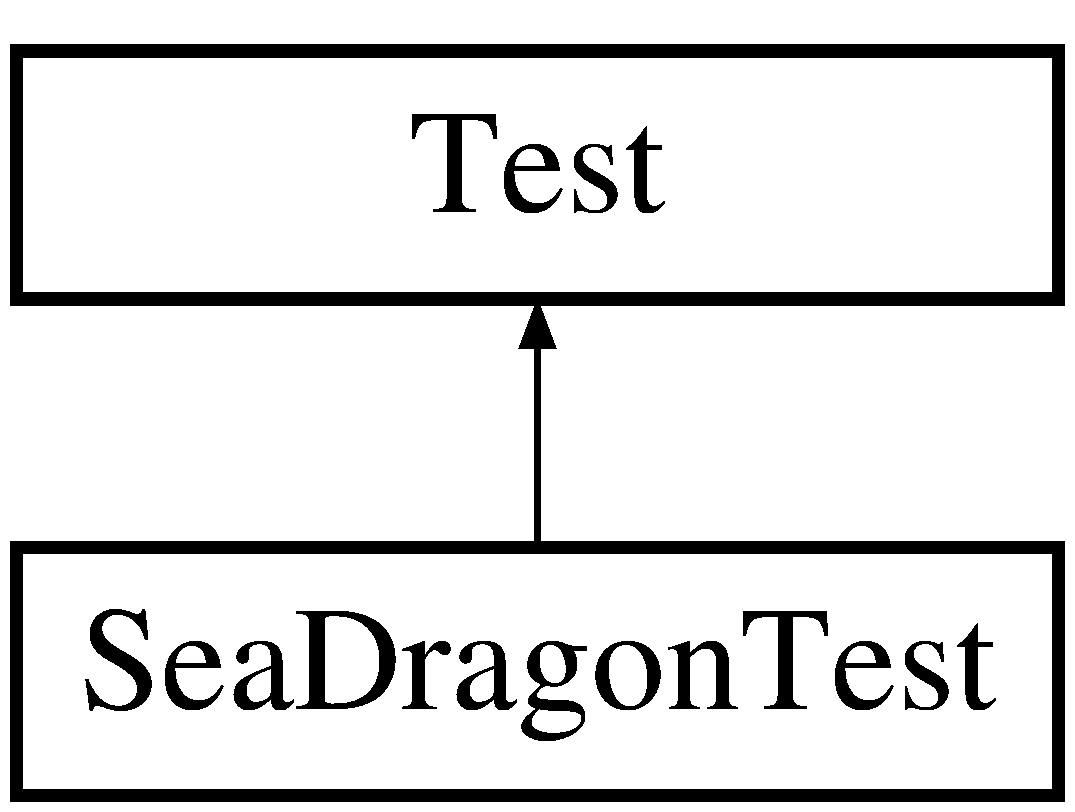
\includegraphics[height=2.000000cm]{class_sea_dragon_test}
\end{center}
\end{figure}


The documentation for this class was generated from the following file\+:\begin{DoxyCompactItemize}
\item 
main\+\_\+test.\+cpp\end{DoxyCompactItemize}

\hypertarget{class_squirrel_monkey}{}\section{Squirrel\+Monkey Class Reference}
\label{class_squirrel_monkey}\index{Squirrel\+Monkey@{Squirrel\+Monkey}}
\subsection*{Public Member Functions}
\begin{DoxyCompactItemize}
\item 
\hyperlink{class_squirrel_monkey_afe630290b17ed0802a1377da5f654629}{Squirrel\+Monkey} ()\hypertarget{class_squirrel_monkey_afe630290b17ed0802a1377da5f654629}{}\label{class_squirrel_monkey_afe630290b17ed0802a1377da5f654629}

\begin{DoxyCompactList}\small\item\em Inisialisasi Hewan. \end{DoxyCompactList}\item 
\hyperlink{class_squirrel_monkey_a591d18d732931da408ed1ff8c81ff753}{$\sim$\+Squirrel\+Monkey} ()\hypertarget{class_squirrel_monkey_a591d18d732931da408ed1ff8c81ff753}{}\label{class_squirrel_monkey_a591d18d732931da408ed1ff8c81ff753}

\begin{DoxyCompactList}\small\item\em Destructor. \end{DoxyCompactList}\item 
string \hyperlink{class_squirrel_monkey_a4336dd1d873b63589b421488ba6717ca}{Get\+Experience} ()\hypertarget{class_squirrel_monkey_a4336dd1d873b63589b421488ba6717ca}{}\label{class_squirrel_monkey_a4336dd1d873b63589b421488ba6717ca}

\begin{DoxyCompactList}\small\item\em Komunikasi dengan hewan. \end{DoxyCompactList}\item 
int \hyperlink{class_squirrel_monkey_a3d33cbedeb2cc2f12715ae456f1dc918}{Get\+Food\+Num} ()
\begin{DoxyCompactList}\small\item\em Jumlah makanan. \end{DoxyCompactList}\item 
char \hyperlink{class_squirrel_monkey_acfb53f4a7d03c8fd41811b70b87b3ce6}{Get\+Render} ()
\begin{DoxyCompactList}\small\item\em Print karakter. \end{DoxyCompactList}\item 
void \hyperlink{class_squirrel_monkey_a79b1ada89d2b5a04ee8fa5970ae74358}{Set\+Enemy} (char cc)
\begin{DoxyCompactList}\small\item\em Set karakter hewan. \end{DoxyCompactList}\item 
char $\ast$ \hyperlink{class_squirrel_monkey_a8669fa3d098c4af3c10f44fdac4ca21e}{Get\+Enemy} ()
\begin{DoxyCompactList}\small\item\em Ambil list musuh. \end{DoxyCompactList}\end{DoxyCompactItemize}
\subsection*{Protected Attributes}
\begin{DoxyCompactItemize}
\item 
int $\ast$ \hyperlink{class_squirrel_monkey_a976f90af80d2665bd2f30340ebc2f8ca}{Type}
\item 
string \hyperlink{class_squirrel_monkey_a2fffa2370eed2fc2e18d9a5f95c50aec}{Famili}
\item 
string \hyperlink{class_squirrel_monkey_a2d5a588234e73bb6a7314bde566df5e4}{Species}
\item 
string \hyperlink{class_squirrel_monkey_ab2bff3349257cff1ca81526e65b14518}{Experience}
\item 
short \hyperlink{class_squirrel_monkey_a000ae715b4b00c9161921859353861d6}{Jenis\+Makanan}
\item 
int \hyperlink{class_squirrel_monkey_a7b042b085902dc1bf3e784adb8a5a61f}{Berat}
\item 
char \hyperlink{class_squirrel_monkey_a46e6c5265b6475baef79e32ea7b0ce43}{Ani\+Char}
\item 
char $\ast$ \hyperlink{class_squirrel_monkey_a8f86426293e656d52b0bee7f1ed1de95}{Enemy\+Char}
\item 
int \hyperlink{class_squirrel_monkey_a68bf6d84b4b0c03126fa172339c80754}{Top\+Enemy}
\end{DoxyCompactItemize}


\subsection{Member Function Documentation}
\index{Squirrel\+Monkey@{Squirrel\+Monkey}!Get\+Enemy@{Get\+Enemy}}
\index{Get\+Enemy@{Get\+Enemy}!Squirrel\+Monkey@{Squirrel\+Monkey}}
\subsubsection[{\texorpdfstring{Get\+Enemy()}{GetEnemy()}}]{\setlength{\rightskip}{0pt plus 5cm}char $\ast$ Squirrel\+Monkey\+::\+Get\+Enemy (
\begin{DoxyParamCaption}
{}
\end{DoxyParamCaption}
)}\hypertarget{class_squirrel_monkey_a8669fa3d098c4af3c10f44fdac4ca21e}{}\label{class_squirrel_monkey_a8669fa3d098c4af3c10f44fdac4ca21e}


Ambil list musuh. 

\begin{DoxyReturn}{Returns}
List Musuh 
\end{DoxyReturn}
\index{Squirrel\+Monkey@{Squirrel\+Monkey}!Get\+Food\+Num@{Get\+Food\+Num}}
\index{Get\+Food\+Num@{Get\+Food\+Num}!Squirrel\+Monkey@{Squirrel\+Monkey}}
\subsubsection[{\texorpdfstring{Get\+Food\+Num()}{GetFoodNum()}}]{\setlength{\rightskip}{0pt plus 5cm}int Squirrel\+Monkey\+::\+Get\+Food\+Num (
\begin{DoxyParamCaption}
{}
\end{DoxyParamCaption}
)}\hypertarget{class_squirrel_monkey_a3d33cbedeb2cc2f12715ae456f1dc918}{}\label{class_squirrel_monkey_a3d33cbedeb2cc2f12715ae456f1dc918}


Jumlah makanan. 

\begin{DoxyReturn}{Returns}
Jumlah makan

Jumlah makanan 
\end{DoxyReturn}
\index{Squirrel\+Monkey@{Squirrel\+Monkey}!Get\+Render@{Get\+Render}}
\index{Get\+Render@{Get\+Render}!Squirrel\+Monkey@{Squirrel\+Monkey}}
\subsubsection[{\texorpdfstring{Get\+Render()}{GetRender()}}]{\setlength{\rightskip}{0pt plus 5cm}char Squirrel\+Monkey\+::\+Get\+Render (
\begin{DoxyParamCaption}
{}
\end{DoxyParamCaption}
)}\hypertarget{class_squirrel_monkey_acfb53f4a7d03c8fd41811b70b87b3ce6}{}\label{class_squirrel_monkey_acfb53f4a7d03c8fd41811b70b87b3ce6}


Print karakter. 

\begin{DoxyReturn}{Returns}
char 
\end{DoxyReturn}
\index{Squirrel\+Monkey@{Squirrel\+Monkey}!Set\+Enemy@{Set\+Enemy}}
\index{Set\+Enemy@{Set\+Enemy}!Squirrel\+Monkey@{Squirrel\+Monkey}}
\subsubsection[{\texorpdfstring{Set\+Enemy(char cc)}{SetEnemy(char cc)}}]{\setlength{\rightskip}{0pt plus 5cm}void Squirrel\+Monkey\+::\+Set\+Enemy (
\begin{DoxyParamCaption}
\item[{char}]{cc}
\end{DoxyParamCaption}
)}\hypertarget{class_squirrel_monkey_a79b1ada89d2b5a04ee8fa5970ae74358}{}\label{class_squirrel_monkey_a79b1ada89d2b5a04ee8fa5970ae74358}


Set karakter hewan. 


\begin{DoxyParams}{Parameters}
{\em cc} & Karakter hewan tsb \\
\hline
\end{DoxyParams}


\subsection{Member Data Documentation}
\index{Squirrel\+Monkey@{Squirrel\+Monkey}!Ani\+Char@{Ani\+Char}}
\index{Ani\+Char@{Ani\+Char}!Squirrel\+Monkey@{Squirrel\+Monkey}}
\subsubsection[{\texorpdfstring{Ani\+Char}{AniChar}}]{\setlength{\rightskip}{0pt plus 5cm}char Squirrel\+Monkey\+::\+Ani\+Char\hspace{0.3cm}{\ttfamily [protected]}}\hypertarget{class_squirrel_monkey_a46e6c5265b6475baef79e32ea7b0ce43}{}\label{class_squirrel_monkey_a46e6c5265b6475baef79e32ea7b0ce43}
Char yang digunakan untuk render \index{Squirrel\+Monkey@{Squirrel\+Monkey}!Berat@{Berat}}
\index{Berat@{Berat}!Squirrel\+Monkey@{Squirrel\+Monkey}}
\subsubsection[{\texorpdfstring{Berat}{Berat}}]{\setlength{\rightskip}{0pt plus 5cm}int Squirrel\+Monkey\+::\+Berat\hspace{0.3cm}{\ttfamily [protected]}}\hypertarget{class_squirrel_monkey_a7b042b085902dc1bf3e784adb8a5a61f}{}\label{class_squirrel_monkey_a7b042b085902dc1bf3e784adb8a5a61f}
Berat hewan \index{Squirrel\+Monkey@{Squirrel\+Monkey}!Enemy\+Char@{Enemy\+Char}}
\index{Enemy\+Char@{Enemy\+Char}!Squirrel\+Monkey@{Squirrel\+Monkey}}
\subsubsection[{\texorpdfstring{Enemy\+Char}{EnemyChar}}]{\setlength{\rightskip}{0pt plus 5cm}char$\ast$ Squirrel\+Monkey\+::\+Enemy\+Char\hspace{0.3cm}{\ttfamily [protected]}}\hypertarget{class_squirrel_monkey_a8f86426293e656d52b0bee7f1ed1de95}{}\label{class_squirrel_monkey_a8f86426293e656d52b0bee7f1ed1de95}
Array of char yang berisi list musuhnya \index{Squirrel\+Monkey@{Squirrel\+Monkey}!Experience@{Experience}}
\index{Experience@{Experience}!Squirrel\+Monkey@{Squirrel\+Monkey}}
\subsubsection[{\texorpdfstring{Experience}{Experience}}]{\setlength{\rightskip}{0pt plus 5cm}string Squirrel\+Monkey\+::\+Experience\hspace{0.3cm}{\ttfamily [protected]}}\hypertarget{class_squirrel_monkey_ab2bff3349257cff1ca81526e65b14518}{}\label{class_squirrel_monkey_ab2bff3349257cff1ca81526e65b14518}
Experience hewan \index{Squirrel\+Monkey@{Squirrel\+Monkey}!Famili@{Famili}}
\index{Famili@{Famili}!Squirrel\+Monkey@{Squirrel\+Monkey}}
\subsubsection[{\texorpdfstring{Famili}{Famili}}]{\setlength{\rightskip}{0pt plus 5cm}string Squirrel\+Monkey\+::\+Famili\hspace{0.3cm}{\ttfamily [protected]}}\hypertarget{class_squirrel_monkey_a2fffa2370eed2fc2e18d9a5f95c50aec}{}\label{class_squirrel_monkey_a2fffa2370eed2fc2e18d9a5f95c50aec}
Family hewan \index{Squirrel\+Monkey@{Squirrel\+Monkey}!Jenis\+Makanan@{Jenis\+Makanan}}
\index{Jenis\+Makanan@{Jenis\+Makanan}!Squirrel\+Monkey@{Squirrel\+Monkey}}
\subsubsection[{\texorpdfstring{Jenis\+Makanan}{JenisMakanan}}]{\setlength{\rightskip}{0pt plus 5cm}short Squirrel\+Monkey\+::\+Jenis\+Makanan\hspace{0.3cm}{\ttfamily [protected]}}\hypertarget{class_squirrel_monkey_a000ae715b4b00c9161921859353861d6}{}\label{class_squirrel_monkey_a000ae715b4b00c9161921859353861d6}
Jenis Makanan hewan. 1 \+: herbifor, 2 \+: karnivor, 3 \+: omnifor \index{Squirrel\+Monkey@{Squirrel\+Monkey}!Species@{Species}}
\index{Species@{Species}!Squirrel\+Monkey@{Squirrel\+Monkey}}
\subsubsection[{\texorpdfstring{Species}{Species}}]{\setlength{\rightskip}{0pt plus 5cm}string Squirrel\+Monkey\+::\+Species\hspace{0.3cm}{\ttfamily [protected]}}\hypertarget{class_squirrel_monkey_a2d5a588234e73bb6a7314bde566df5e4}{}\label{class_squirrel_monkey_a2d5a588234e73bb6a7314bde566df5e4}
Species hewan \index{Squirrel\+Monkey@{Squirrel\+Monkey}!Top\+Enemy@{Top\+Enemy}}
\index{Top\+Enemy@{Top\+Enemy}!Squirrel\+Monkey@{Squirrel\+Monkey}}
\subsubsection[{\texorpdfstring{Top\+Enemy}{TopEnemy}}]{\setlength{\rightskip}{0pt plus 5cm}int Squirrel\+Monkey\+::\+Top\+Enemy\hspace{0.3cm}{\ttfamily [protected]}}\hypertarget{class_squirrel_monkey_a68bf6d84b4b0c03126fa172339c80754}{}\label{class_squirrel_monkey_a68bf6d84b4b0c03126fa172339c80754}
Pointer Enemy\+Char yang available \index{Squirrel\+Monkey@{Squirrel\+Monkey}!Type@{Type}}
\index{Type@{Type}!Squirrel\+Monkey@{Squirrel\+Monkey}}
\subsubsection[{\texorpdfstring{Type}{Type}}]{\setlength{\rightskip}{0pt plus 5cm}int$\ast$ Squirrel\+Monkey\+::\+Type\hspace{0.3cm}{\ttfamily [protected]}}\hypertarget{class_squirrel_monkey_a976f90af80d2665bd2f30340ebc2f8ca}{}\label{class_squirrel_monkey_a976f90af80d2665bd2f30340ebc2f8ca}
Type habitat hewan. 0 \+: darat, 1 \+: udara, 2 \+: air 

The documentation for this class was generated from the following files\+:\begin{DoxyCompactItemize}
\item 
squirrelmonkey.\+h\item 
squirrelmonkey.\+cpp\end{DoxyCompactItemize}

\hypertarget{class_squirrel_monkey_test}{}\section{Squirrel\+Monkey\+Test Class Reference}
\label{class_squirrel_monkey_test}\index{Squirrel\+Monkey\+Test@{Squirrel\+Monkey\+Test}}
Inheritance diagram for Squirrel\+Monkey\+Test\+:\begin{figure}[H]
\begin{center}
\leavevmode
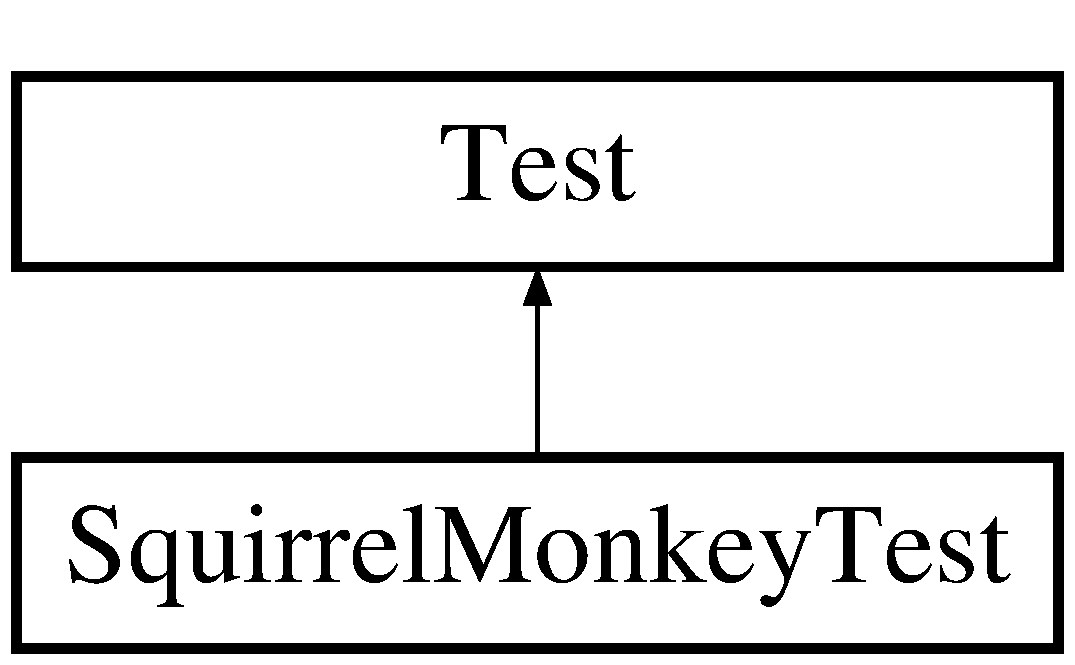
\includegraphics[height=2.000000cm]{class_squirrel_monkey_test}
\end{center}
\end{figure}


The documentation for this class was generated from the following file\+:\begin{DoxyCompactItemize}
\item 
main\+\_\+test.\+cpp\end{DoxyCompactItemize}

\hypertarget{class_tiger}{}\section{Tiger Class Reference}
\label{class_tiger}\index{Tiger@{Tiger}}
\subsection*{Public Member Functions}
\begin{DoxyCompactItemize}
\item 
\hyperlink{class_tiger_ab2b455a0cdbd21f2052eef2a176f0eeb}{Tiger} ()\hypertarget{class_tiger_ab2b455a0cdbd21f2052eef2a176f0eeb}{}\label{class_tiger_ab2b455a0cdbd21f2052eef2a176f0eeb}

\begin{DoxyCompactList}\small\item\em Inisialisasi Hewan. \end{DoxyCompactList}\item 
\hyperlink{class_tiger_acb6310bff243b1d14ea8f783a22c62b4}{$\sim$\+Tiger} ()\hypertarget{class_tiger_acb6310bff243b1d14ea8f783a22c62b4}{}\label{class_tiger_acb6310bff243b1d14ea8f783a22c62b4}

\begin{DoxyCompactList}\small\item\em Destructor. \end{DoxyCompactList}\item 
string \hyperlink{class_tiger_acd585f0b4c5388b87626e0d0a8434daa}{Get\+Experience} ()\hypertarget{class_tiger_acd585f0b4c5388b87626e0d0a8434daa}{}\label{class_tiger_acd585f0b4c5388b87626e0d0a8434daa}

\begin{DoxyCompactList}\small\item\em Komunikasi dengan hewan. \end{DoxyCompactList}\item 
int \hyperlink{class_tiger_a71039b4cfa967f7c2060e7c4b198e033}{Get\+Food\+Num} ()
\begin{DoxyCompactList}\small\item\em Jumlah makanan. \end{DoxyCompactList}\item 
char \hyperlink{class_tiger_a8a6d245d21eb4407c299189ca1c52e1b}{Get\+Render} ()
\begin{DoxyCompactList}\small\item\em Print karakter. \end{DoxyCompactList}\item 
void \hyperlink{class_tiger_aeee182899a035f0471c761fa073e19f9}{Set\+Enemy} (char cc)
\begin{DoxyCompactList}\small\item\em Set karakter hewan. \end{DoxyCompactList}\item 
char $\ast$ \hyperlink{class_tiger_a053a83818fe6415121e01d726a04dbd5}{Get\+Enemy} ()
\begin{DoxyCompactList}\small\item\em Ambil list musuh. \end{DoxyCompactList}\end{DoxyCompactItemize}
\subsection*{Protected Attributes}
\begin{DoxyCompactItemize}
\item 
int $\ast$ \hyperlink{class_tiger_afada3a13aec9f2a57bd878686b4de88d}{Type}
\item 
string \hyperlink{class_tiger_a508ded11631e75ca8def9d08382fe53e}{Famili}
\item 
string \hyperlink{class_tiger_a8311889e0a734ced0a434b4d244ed0ec}{Species}
\item 
string \hyperlink{class_tiger_a94e7d699e66aa4d3027f64837c2d5f11}{Experience}
\item 
short \hyperlink{class_tiger_afb03e7b01934b4b95c021986c8ca9dae}{Jenis\+Makanan}
\item 
int \hyperlink{class_tiger_ad84a8d5962f7de935246be3682dbdd15}{Berat}
\item 
char \hyperlink{class_tiger_a5a0cb7d341ab62aeff1f9762f24d4bf9}{Ani\+Char}
\item 
char $\ast$ \hyperlink{class_tiger_a418b4305ac370e8a64621c24984115a1}{Enemy\+Char}
\item 
int \hyperlink{class_tiger_aeb3c4e72880d8be516844dd0898e71f4}{Top\+Enemy}
\end{DoxyCompactItemize}


\subsection{Member Function Documentation}
\index{Tiger@{Tiger}!Get\+Enemy@{Get\+Enemy}}
\index{Get\+Enemy@{Get\+Enemy}!Tiger@{Tiger}}
\subsubsection[{\texorpdfstring{Get\+Enemy()}{GetEnemy()}}]{\setlength{\rightskip}{0pt plus 5cm}char $\ast$ Tiger\+::\+Get\+Enemy (
\begin{DoxyParamCaption}
{}
\end{DoxyParamCaption}
)}\hypertarget{class_tiger_a053a83818fe6415121e01d726a04dbd5}{}\label{class_tiger_a053a83818fe6415121e01d726a04dbd5}


Ambil list musuh. 

\begin{DoxyReturn}{Returns}
List Musuh 
\end{DoxyReturn}
\index{Tiger@{Tiger}!Get\+Food\+Num@{Get\+Food\+Num}}
\index{Get\+Food\+Num@{Get\+Food\+Num}!Tiger@{Tiger}}
\subsubsection[{\texorpdfstring{Get\+Food\+Num()}{GetFoodNum()}}]{\setlength{\rightskip}{0pt plus 5cm}int Tiger\+::\+Get\+Food\+Num (
\begin{DoxyParamCaption}
{}
\end{DoxyParamCaption}
)}\hypertarget{class_tiger_a71039b4cfa967f7c2060e7c4b198e033}{}\label{class_tiger_a71039b4cfa967f7c2060e7c4b198e033}


Jumlah makanan. 

\begin{DoxyReturn}{Returns}
Jumlah makan

Jumlah makanan 
\end{DoxyReturn}
\index{Tiger@{Tiger}!Get\+Render@{Get\+Render}}
\index{Get\+Render@{Get\+Render}!Tiger@{Tiger}}
\subsubsection[{\texorpdfstring{Get\+Render()}{GetRender()}}]{\setlength{\rightskip}{0pt plus 5cm}char Tiger\+::\+Get\+Render (
\begin{DoxyParamCaption}
{}
\end{DoxyParamCaption}
)}\hypertarget{class_tiger_a8a6d245d21eb4407c299189ca1c52e1b}{}\label{class_tiger_a8a6d245d21eb4407c299189ca1c52e1b}


Print karakter. 

\begin{DoxyReturn}{Returns}
char 
\end{DoxyReturn}
\index{Tiger@{Tiger}!Set\+Enemy@{Set\+Enemy}}
\index{Set\+Enemy@{Set\+Enemy}!Tiger@{Tiger}}
\subsubsection[{\texorpdfstring{Set\+Enemy(char cc)}{SetEnemy(char cc)}}]{\setlength{\rightskip}{0pt plus 5cm}void Tiger\+::\+Set\+Enemy (
\begin{DoxyParamCaption}
\item[{char}]{cc}
\end{DoxyParamCaption}
)}\hypertarget{class_tiger_aeee182899a035f0471c761fa073e19f9}{}\label{class_tiger_aeee182899a035f0471c761fa073e19f9}


Set karakter hewan. 


\begin{DoxyParams}{Parameters}
{\em cc} & Karakter hewan tsb \\
\hline
\end{DoxyParams}


\subsection{Member Data Documentation}
\index{Tiger@{Tiger}!Ani\+Char@{Ani\+Char}}
\index{Ani\+Char@{Ani\+Char}!Tiger@{Tiger}}
\subsubsection[{\texorpdfstring{Ani\+Char}{AniChar}}]{\setlength{\rightskip}{0pt plus 5cm}char Tiger\+::\+Ani\+Char\hspace{0.3cm}{\ttfamily [protected]}}\hypertarget{class_tiger_a5a0cb7d341ab62aeff1f9762f24d4bf9}{}\label{class_tiger_a5a0cb7d341ab62aeff1f9762f24d4bf9}
Char yang digunakan untuk render \index{Tiger@{Tiger}!Berat@{Berat}}
\index{Berat@{Berat}!Tiger@{Tiger}}
\subsubsection[{\texorpdfstring{Berat}{Berat}}]{\setlength{\rightskip}{0pt plus 5cm}int Tiger\+::\+Berat\hspace{0.3cm}{\ttfamily [protected]}}\hypertarget{class_tiger_ad84a8d5962f7de935246be3682dbdd15}{}\label{class_tiger_ad84a8d5962f7de935246be3682dbdd15}
Berat hewan \index{Tiger@{Tiger}!Enemy\+Char@{Enemy\+Char}}
\index{Enemy\+Char@{Enemy\+Char}!Tiger@{Tiger}}
\subsubsection[{\texorpdfstring{Enemy\+Char}{EnemyChar}}]{\setlength{\rightskip}{0pt plus 5cm}char$\ast$ Tiger\+::\+Enemy\+Char\hspace{0.3cm}{\ttfamily [protected]}}\hypertarget{class_tiger_a418b4305ac370e8a64621c24984115a1}{}\label{class_tiger_a418b4305ac370e8a64621c24984115a1}
Array of char yang berisi list musuhnya \index{Tiger@{Tiger}!Experience@{Experience}}
\index{Experience@{Experience}!Tiger@{Tiger}}
\subsubsection[{\texorpdfstring{Experience}{Experience}}]{\setlength{\rightskip}{0pt plus 5cm}string Tiger\+::\+Experience\hspace{0.3cm}{\ttfamily [protected]}}\hypertarget{class_tiger_a94e7d699e66aa4d3027f64837c2d5f11}{}\label{class_tiger_a94e7d699e66aa4d3027f64837c2d5f11}
Experience hewan \index{Tiger@{Tiger}!Famili@{Famili}}
\index{Famili@{Famili}!Tiger@{Tiger}}
\subsubsection[{\texorpdfstring{Famili}{Famili}}]{\setlength{\rightskip}{0pt plus 5cm}string Tiger\+::\+Famili\hspace{0.3cm}{\ttfamily [protected]}}\hypertarget{class_tiger_a508ded11631e75ca8def9d08382fe53e}{}\label{class_tiger_a508ded11631e75ca8def9d08382fe53e}
Family hewan \index{Tiger@{Tiger}!Jenis\+Makanan@{Jenis\+Makanan}}
\index{Jenis\+Makanan@{Jenis\+Makanan}!Tiger@{Tiger}}
\subsubsection[{\texorpdfstring{Jenis\+Makanan}{JenisMakanan}}]{\setlength{\rightskip}{0pt plus 5cm}short Tiger\+::\+Jenis\+Makanan\hspace{0.3cm}{\ttfamily [protected]}}\hypertarget{class_tiger_afb03e7b01934b4b95c021986c8ca9dae}{}\label{class_tiger_afb03e7b01934b4b95c021986c8ca9dae}
Jenis Makanan hewan. 1 \+: herbifor, 2 \+: karnivor, 3 \+: omnifor \index{Tiger@{Tiger}!Species@{Species}}
\index{Species@{Species}!Tiger@{Tiger}}
\subsubsection[{\texorpdfstring{Species}{Species}}]{\setlength{\rightskip}{0pt plus 5cm}string Tiger\+::\+Species\hspace{0.3cm}{\ttfamily [protected]}}\hypertarget{class_tiger_a8311889e0a734ced0a434b4d244ed0ec}{}\label{class_tiger_a8311889e0a734ced0a434b4d244ed0ec}
Species hewan \index{Tiger@{Tiger}!Top\+Enemy@{Top\+Enemy}}
\index{Top\+Enemy@{Top\+Enemy}!Tiger@{Tiger}}
\subsubsection[{\texorpdfstring{Top\+Enemy}{TopEnemy}}]{\setlength{\rightskip}{0pt plus 5cm}int Tiger\+::\+Top\+Enemy\hspace{0.3cm}{\ttfamily [protected]}}\hypertarget{class_tiger_aeb3c4e72880d8be516844dd0898e71f4}{}\label{class_tiger_aeb3c4e72880d8be516844dd0898e71f4}
Pointer Enemy\+Char yang available \index{Tiger@{Tiger}!Type@{Type}}
\index{Type@{Type}!Tiger@{Tiger}}
\subsubsection[{\texorpdfstring{Type}{Type}}]{\setlength{\rightskip}{0pt plus 5cm}int$\ast$ Tiger\+::\+Type\hspace{0.3cm}{\ttfamily [protected]}}\hypertarget{class_tiger_afada3a13aec9f2a57bd878686b4de88d}{}\label{class_tiger_afada3a13aec9f2a57bd878686b4de88d}
Type habitat hewan. 0 \+: darat, 1 \+: udara, 2 \+: air 

The documentation for this class was generated from the following files\+:\begin{DoxyCompactItemize}
\item 
tiger.\+h\item 
tiger.\+cpp\end{DoxyCompactItemize}

\hypertarget{class_tiger_test}{}\section{Tiger\+Test Class Reference}
\label{class_tiger_test}\index{Tiger\+Test@{Tiger\+Test}}
Inheritance diagram for Tiger\+Test\+:\begin{figure}[H]
\begin{center}
\leavevmode
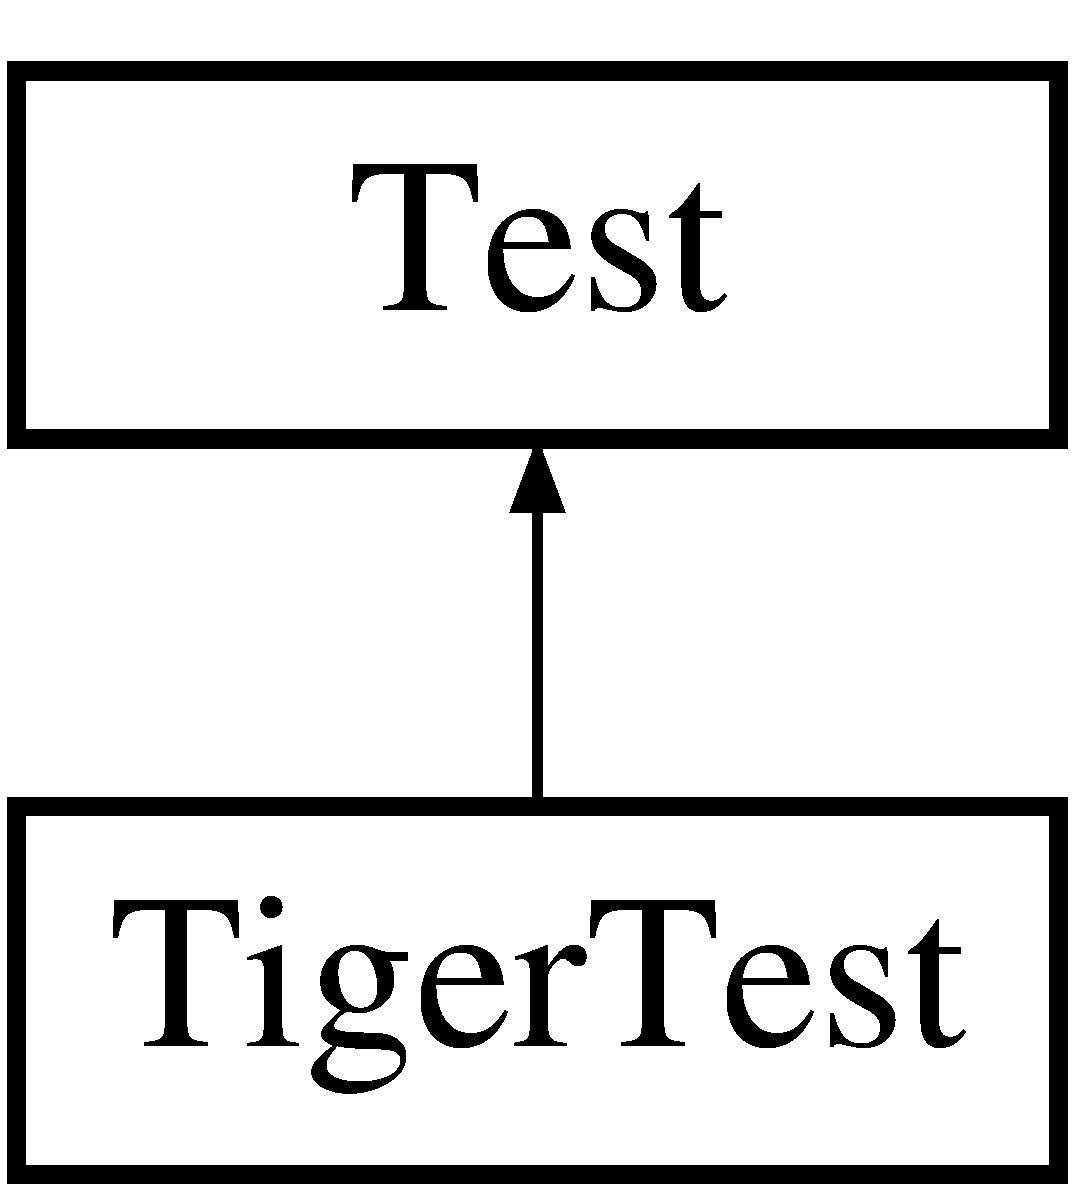
\includegraphics[height=2.000000cm]{class_tiger_test}
\end{center}
\end{figure}


The documentation for this class was generated from the following file\+:\begin{DoxyCompactItemize}
\item 
main\+\_\+test.\+cpp\end{DoxyCompactItemize}

\hypertarget{class_water_habitat}{}\section{Water\+Habitat Class Reference}
\label{class_water_habitat}\index{Water\+Habitat@{Water\+Habitat}}
\subsection*{Public Member Functions}
\begin{DoxyCompactItemize}
\item 
\hyperlink{class_water_habitat_a57a0d15fae5e17531835be2284df0fd1}{Water\+Habitat} ()
\begin{DoxyCompactList}\small\item\em constructor \end{DoxyCompactList}\item 
virtual \hyperlink{class_water_habitat_abf6341b18b2fe62110998db3ffbde4b7}{$\sim$\+Water\+Habitat} ()\hypertarget{class_water_habitat_abf6341b18b2fe62110998db3ffbde4b7}{}\label{class_water_habitat_abf6341b18b2fe62110998db3ffbde4b7}

\begin{DoxyCompactList}\small\item\em Destructor. \end{DoxyCompactList}\item 
char \hyperlink{class_water_habitat_af580b4a2a182052805b47b8ef9eded1e}{Get\+Render} ()
\begin{DoxyCompactList}\small\item\em render nawn \end{DoxyCompactList}\end{DoxyCompactItemize}


\subsection{Constructor \& Destructor Documentation}
\index{Water\+Habitat@{Water\+Habitat}!Water\+Habitat@{Water\+Habitat}}
\index{Water\+Habitat@{Water\+Habitat}!Water\+Habitat@{Water\+Habitat}}
\subsubsection[{\texorpdfstring{Water\+Habitat()}{WaterHabitat()}}]{\setlength{\rightskip}{0pt plus 5cm}Water\+Habitat\+::\+Water\+Habitat (
\begin{DoxyParamCaption}
{}
\end{DoxyParamCaption}
)}\hypertarget{class_water_habitat_a57a0d15fae5e17531835be2284df0fd1}{}\label{class_water_habitat_a57a0d15fae5e17531835be2284df0fd1}


constructor 


\begin{DoxyParams}{Parameters}
{\em posx} & posisi x \\
\hline
{\em posy} & posisi y \\
\hline
\end{DoxyParams}


\subsection{Member Function Documentation}
\index{Water\+Habitat@{Water\+Habitat}!Get\+Render@{Get\+Render}}
\index{Get\+Render@{Get\+Render}!Water\+Habitat@{Water\+Habitat}}
\subsubsection[{\texorpdfstring{Get\+Render()}{GetRender()}}]{\setlength{\rightskip}{0pt plus 5cm}char Water\+Habitat\+::\+Get\+Render (
\begin{DoxyParamCaption}
{}
\end{DoxyParamCaption}
)}\hypertarget{class_water_habitat_af580b4a2a182052805b47b8ef9eded1e}{}\label{class_water_habitat_af580b4a2a182052805b47b8ef9eded1e}


render nawn 


\begin{DoxyParams}{Parameters}
{\em cc} & nawnnawn \\
\hline
\end{DoxyParams}


The documentation for this class was generated from the following files\+:\begin{DoxyCompactItemize}
\item 
water\+\_\+habitat.\+h\item 
water\+\_\+habitat.\+cpp\end{DoxyCompactItemize}

\hypertarget{class_water_habitat_test}{}\section{Water\+Habitat\+Test Class Reference}
\label{class_water_habitat_test}\index{Water\+Habitat\+Test@{Water\+Habitat\+Test}}
Inheritance diagram for Water\+Habitat\+Test\+:\begin{figure}[H]
\begin{center}
\leavevmode
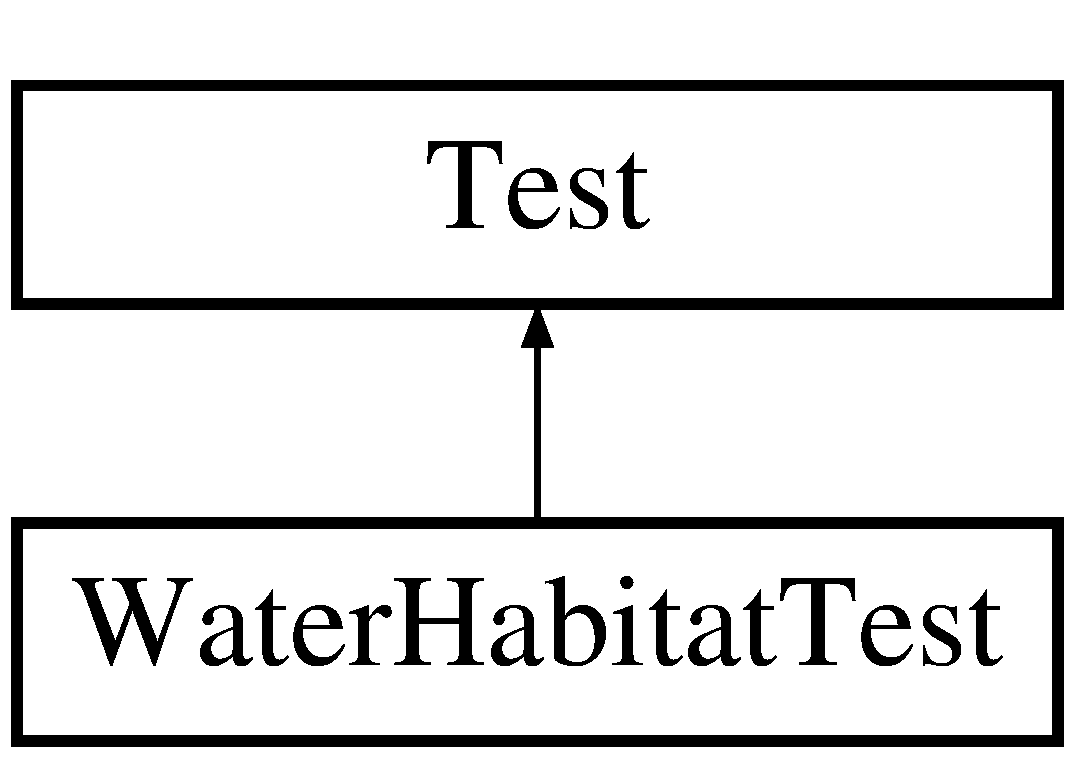
\includegraphics[height=2.000000cm]{class_water_habitat_test}
\end{center}
\end{figure}


The documentation for this class was generated from the following file\+:\begin{DoxyCompactItemize}
\item 
main\+\_\+test.\+cpp\end{DoxyCompactItemize}

\hypertarget{class_whale}{}\section{Whale Class Reference}
\label{class_whale}\index{Whale@{Whale}}
Inheritance diagram for Whale\+:\begin{figure}[H]
\begin{center}
\leavevmode
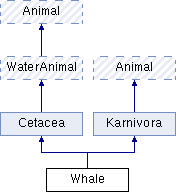
\includegraphics[height=4.000000cm]{class_whale}
\end{center}
\end{figure}
\subsection*{Public Member Functions}
\begin{DoxyCompactItemize}
\item 
\hyperlink{class_whale_a1a3ee57b92f6fb72ccf0fa12ea118cd7}{Whale} ()\hypertarget{class_whale_a1a3ee57b92f6fb72ccf0fa12ea118cd7}{}\label{class_whale_a1a3ee57b92f6fb72ccf0fa12ea118cd7}

\begin{DoxyCompactList}\small\item\em Inisialisasi Hewan. \end{DoxyCompactList}\end{DoxyCompactItemize}
\subsection*{Additional Inherited Members}


The documentation for this class was generated from the following files\+:\begin{DoxyCompactItemize}
\item 
water\+\_\+animal.\+h\item 
water\+\_\+animal.\+cpp\end{DoxyCompactItemize}

\hypertarget{class_whale_test}{}\section{Whale\+Test Class Reference}
\label{class_whale_test}\index{Whale\+Test@{Whale\+Test}}
Inheritance diagram for Whale\+Test\+:\begin{figure}[H]
\begin{center}
\leavevmode
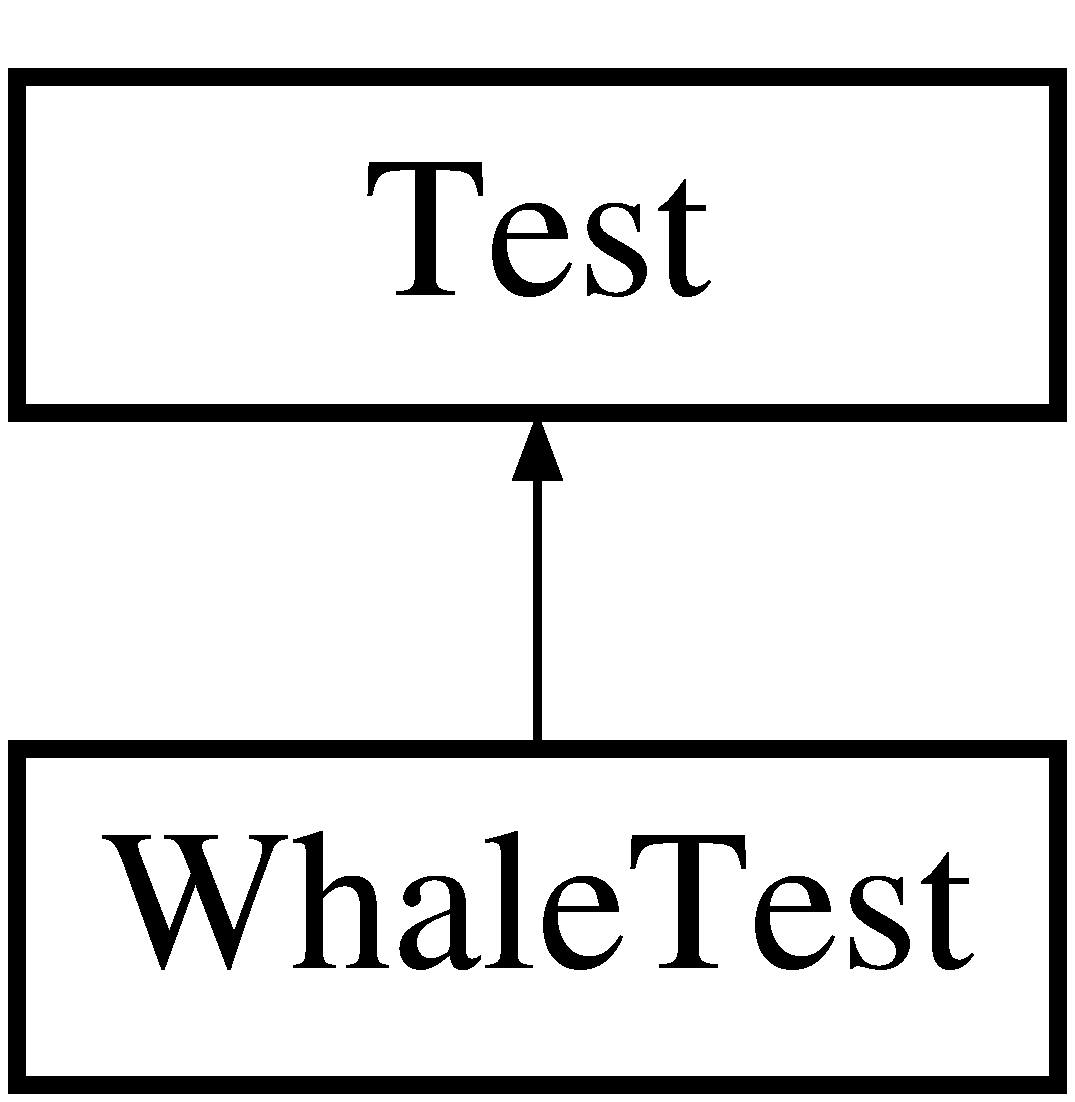
\includegraphics[height=2.000000cm]{class_whale_test}
\end{center}
\end{figure}


The documentation for this class was generated from the following file\+:\begin{DoxyCompactItemize}
\item 
main\+\_\+test.\+cpp\end{DoxyCompactItemize}

\hypertarget{class_white_shark}{}\section{White\+Shark Class Reference}
\label{class_white_shark}\index{White\+Shark@{White\+Shark}}
Inheritance diagram for White\+Shark\+:\begin{figure}[H]
\begin{center}
\leavevmode
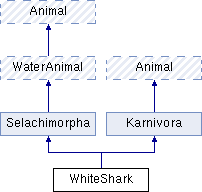
\includegraphics[height=4.000000cm]{class_white_shark}
\end{center}
\end{figure}
\subsection*{Public Member Functions}
\begin{DoxyCompactItemize}
\item 
\hyperlink{class_white_shark_abd3e920a0808c805c07350003157057c}{White\+Shark} ()\hypertarget{class_white_shark_abd3e920a0808c805c07350003157057c}{}\label{class_white_shark_abd3e920a0808c805c07350003157057c}

\begin{DoxyCompactList}\small\item\em Inisialisasi Hewan. \end{DoxyCompactList}\end{DoxyCompactItemize}
\subsection*{Additional Inherited Members}


The documentation for this class was generated from the following files\+:\begin{DoxyCompactItemize}
\item 
water\+\_\+animal.\+h\item 
water\+\_\+animal.\+cpp\end{DoxyCompactItemize}

\hypertarget{class_white_shark_test}{}\section{White\+Shark\+Test Class Reference}
\label{class_white_shark_test}\index{White\+Shark\+Test@{White\+Shark\+Test}}
Inheritance diagram for White\+Shark\+Test\+:\begin{figure}[H]
\begin{center}
\leavevmode
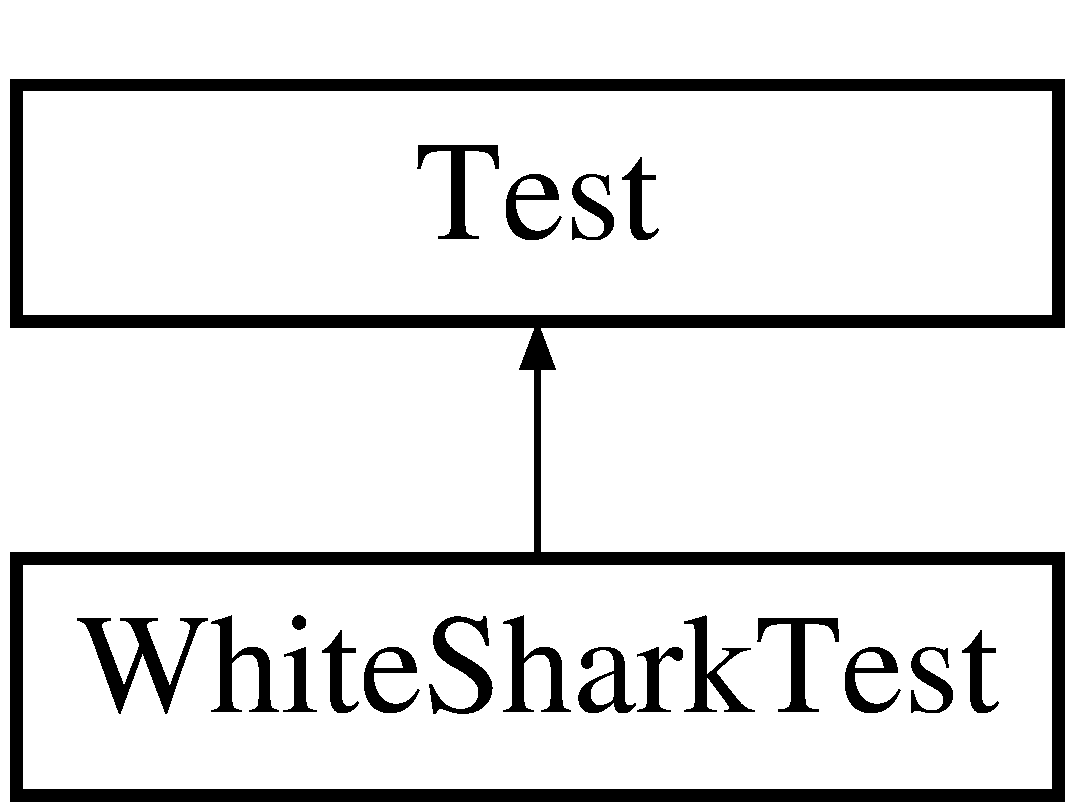
\includegraphics[height=2.000000cm]{class_white_shark_test}
\end{center}
\end{figure}


The documentation for this class was generated from the following file\+:\begin{DoxyCompactItemize}
\item 
main\+\_\+test.\+cpp\end{DoxyCompactItemize}

\hypertarget{class_zebra}{}\section{Zebra Class Reference}
\label{class_zebra}\index{Zebra@{Zebra}}
\subsection*{Public Member Functions}
\begin{DoxyCompactItemize}
\item 
\hyperlink{class_zebra_a06481320d8c665bb5f39e85f83c14ca5}{Zebra} ()\hypertarget{class_zebra_a06481320d8c665bb5f39e85f83c14ca5}{}\label{class_zebra_a06481320d8c665bb5f39e85f83c14ca5}

\begin{DoxyCompactList}\small\item\em Constructor. \end{DoxyCompactList}\item 
\hyperlink{class_zebra_a888564ecb889c3c897267b6619deeb6c}{$\sim$\+Zebra} ()\hypertarget{class_zebra_a888564ecb889c3c897267b6619deeb6c}{}\label{class_zebra_a888564ecb889c3c897267b6619deeb6c}

\begin{DoxyCompactList}\small\item\em Destructor. \end{DoxyCompactList}\item 
string \hyperlink{class_zebra_a6d99c6b3b8e69282eec191982a1922e8}{Get\+Experience} ()\hypertarget{class_zebra_a6d99c6b3b8e69282eec191982a1922e8}{}\label{class_zebra_a6d99c6b3b8e69282eec191982a1922e8}

\begin{DoxyCompactList}\small\item\em Komunikasi dengan hewan. \end{DoxyCompactList}\item 
int \hyperlink{class_zebra_a7ad579e63018f0d666b9d49ddcc01b01}{Get\+Food\+Num} ()
\begin{DoxyCompactList}\small\item\em Jumlah makanan. \end{DoxyCompactList}\item 
char \hyperlink{class_zebra_a264f0cd18f38fc81466d867e08e61806}{Get\+Render} ()
\begin{DoxyCompactList}\small\item\em Print karakter. \end{DoxyCompactList}\item 
void \hyperlink{class_zebra_a110c8832246ce8e762fddff02ffec54e}{Set\+Enemy} (char cc)
\begin{DoxyCompactList}\small\item\em Set karakter hewan. \end{DoxyCompactList}\item 
char $\ast$ \hyperlink{class_zebra_a2e7d4a246b1ed6eb3377f475087c36f0}{Get\+Enemy} ()
\begin{DoxyCompactList}\small\item\em Ambil list musuh. \end{DoxyCompactList}\end{DoxyCompactItemize}
\subsection*{Protected Attributes}
\begin{DoxyCompactItemize}
\item 
int $\ast$ \hyperlink{class_zebra_a6794a0b724c4bc903f225b9b0a04c841}{Type}
\item 
string \hyperlink{class_zebra_afd28ca34e1bbf0e7ef6ae41f697345d2}{Famili}
\item 
string \hyperlink{class_zebra_a0d6e5b92efa4df0f092caf24c5015491}{Species}
\item 
string \hyperlink{class_zebra_a9be71c3f041c760f4096179647f21532}{Experience}
\item 
short \hyperlink{class_zebra_af50d97630fd5fdbb3cb7f977e8689575}{Jenis\+Makanan}
\item 
int \hyperlink{class_zebra_ae450c8048eda3d54f3dc2ec7eb92d79f}{Berat}
\item 
char \hyperlink{class_zebra_aec6d713965ae1fcb374d9911b4880b29}{Ani\+Char}
\item 
char $\ast$ \hyperlink{class_zebra_a3caeeff6684cd124449f2717787bed00}{Enemy\+Char}
\item 
int \hyperlink{class_zebra_a0d13a21f03c66cc28a7b1085f4e05449}{Top\+Enemy}
\end{DoxyCompactItemize}


\subsection{Member Function Documentation}
\index{Zebra@{Zebra}!Get\+Enemy@{Get\+Enemy}}
\index{Get\+Enemy@{Get\+Enemy}!Zebra@{Zebra}}
\subsubsection[{\texorpdfstring{Get\+Enemy()}{GetEnemy()}}]{\setlength{\rightskip}{0pt plus 5cm}char $\ast$ Zebra\+::\+Get\+Enemy (
\begin{DoxyParamCaption}
{}
\end{DoxyParamCaption}
)}\hypertarget{class_zebra_a2e7d4a246b1ed6eb3377f475087c36f0}{}\label{class_zebra_a2e7d4a246b1ed6eb3377f475087c36f0}


Ambil list musuh. 

\begin{DoxyReturn}{Returns}
List Musuh 
\end{DoxyReturn}
\index{Zebra@{Zebra}!Get\+Food\+Num@{Get\+Food\+Num}}
\index{Get\+Food\+Num@{Get\+Food\+Num}!Zebra@{Zebra}}
\subsubsection[{\texorpdfstring{Get\+Food\+Num()}{GetFoodNum()}}]{\setlength{\rightskip}{0pt plus 5cm}int Zebra\+::\+Get\+Food\+Num (
\begin{DoxyParamCaption}
{}
\end{DoxyParamCaption}
)}\hypertarget{class_zebra_a7ad579e63018f0d666b9d49ddcc01b01}{}\label{class_zebra_a7ad579e63018f0d666b9d49ddcc01b01}


Jumlah makanan. 

\begin{DoxyReturn}{Returns}
Jumlah makan

Jumlah makanan 
\end{DoxyReturn}
\index{Zebra@{Zebra}!Get\+Render@{Get\+Render}}
\index{Get\+Render@{Get\+Render}!Zebra@{Zebra}}
\subsubsection[{\texorpdfstring{Get\+Render()}{GetRender()}}]{\setlength{\rightskip}{0pt plus 5cm}char Zebra\+::\+Get\+Render (
\begin{DoxyParamCaption}
{}
\end{DoxyParamCaption}
)}\hypertarget{class_zebra_a264f0cd18f38fc81466d867e08e61806}{}\label{class_zebra_a264f0cd18f38fc81466d867e08e61806}


Print karakter. 

\begin{DoxyReturn}{Returns}
char 
\end{DoxyReturn}
\index{Zebra@{Zebra}!Set\+Enemy@{Set\+Enemy}}
\index{Set\+Enemy@{Set\+Enemy}!Zebra@{Zebra}}
\subsubsection[{\texorpdfstring{Set\+Enemy(char cc)}{SetEnemy(char cc)}}]{\setlength{\rightskip}{0pt plus 5cm}void Zebra\+::\+Set\+Enemy (
\begin{DoxyParamCaption}
\item[{char}]{cc}
\end{DoxyParamCaption}
)}\hypertarget{class_zebra_a110c8832246ce8e762fddff02ffec54e}{}\label{class_zebra_a110c8832246ce8e762fddff02ffec54e}


Set karakter hewan. 


\begin{DoxyParams}{Parameters}
{\em cc} & Karakter hewan tsb \\
\hline
\end{DoxyParams}


\subsection{Member Data Documentation}
\index{Zebra@{Zebra}!Ani\+Char@{Ani\+Char}}
\index{Ani\+Char@{Ani\+Char}!Zebra@{Zebra}}
\subsubsection[{\texorpdfstring{Ani\+Char}{AniChar}}]{\setlength{\rightskip}{0pt plus 5cm}char Zebra\+::\+Ani\+Char\hspace{0.3cm}{\ttfamily [protected]}}\hypertarget{class_zebra_aec6d713965ae1fcb374d9911b4880b29}{}\label{class_zebra_aec6d713965ae1fcb374d9911b4880b29}
Char yang digunakan untuk render \index{Zebra@{Zebra}!Berat@{Berat}}
\index{Berat@{Berat}!Zebra@{Zebra}}
\subsubsection[{\texorpdfstring{Berat}{Berat}}]{\setlength{\rightskip}{0pt plus 5cm}int Zebra\+::\+Berat\hspace{0.3cm}{\ttfamily [protected]}}\hypertarget{class_zebra_ae450c8048eda3d54f3dc2ec7eb92d79f}{}\label{class_zebra_ae450c8048eda3d54f3dc2ec7eb92d79f}
Berat hewan \index{Zebra@{Zebra}!Enemy\+Char@{Enemy\+Char}}
\index{Enemy\+Char@{Enemy\+Char}!Zebra@{Zebra}}
\subsubsection[{\texorpdfstring{Enemy\+Char}{EnemyChar}}]{\setlength{\rightskip}{0pt plus 5cm}char$\ast$ Zebra\+::\+Enemy\+Char\hspace{0.3cm}{\ttfamily [protected]}}\hypertarget{class_zebra_a3caeeff6684cd124449f2717787bed00}{}\label{class_zebra_a3caeeff6684cd124449f2717787bed00}
Array of char yang berisi list musuhnya \index{Zebra@{Zebra}!Experience@{Experience}}
\index{Experience@{Experience}!Zebra@{Zebra}}
\subsubsection[{\texorpdfstring{Experience}{Experience}}]{\setlength{\rightskip}{0pt plus 5cm}string Zebra\+::\+Experience\hspace{0.3cm}{\ttfamily [protected]}}\hypertarget{class_zebra_a9be71c3f041c760f4096179647f21532}{}\label{class_zebra_a9be71c3f041c760f4096179647f21532}
Experience hewan \index{Zebra@{Zebra}!Famili@{Famili}}
\index{Famili@{Famili}!Zebra@{Zebra}}
\subsubsection[{\texorpdfstring{Famili}{Famili}}]{\setlength{\rightskip}{0pt plus 5cm}string Zebra\+::\+Famili\hspace{0.3cm}{\ttfamily [protected]}}\hypertarget{class_zebra_afd28ca34e1bbf0e7ef6ae41f697345d2}{}\label{class_zebra_afd28ca34e1bbf0e7ef6ae41f697345d2}
Family hewan \index{Zebra@{Zebra}!Jenis\+Makanan@{Jenis\+Makanan}}
\index{Jenis\+Makanan@{Jenis\+Makanan}!Zebra@{Zebra}}
\subsubsection[{\texorpdfstring{Jenis\+Makanan}{JenisMakanan}}]{\setlength{\rightskip}{0pt plus 5cm}short Zebra\+::\+Jenis\+Makanan\hspace{0.3cm}{\ttfamily [protected]}}\hypertarget{class_zebra_af50d97630fd5fdbb3cb7f977e8689575}{}\label{class_zebra_af50d97630fd5fdbb3cb7f977e8689575}
Jenis Makanan hewan. 1 \+: herbifor, 2 \+: karnivor, 3 \+: omnifor \index{Zebra@{Zebra}!Species@{Species}}
\index{Species@{Species}!Zebra@{Zebra}}
\subsubsection[{\texorpdfstring{Species}{Species}}]{\setlength{\rightskip}{0pt plus 5cm}string Zebra\+::\+Species\hspace{0.3cm}{\ttfamily [protected]}}\hypertarget{class_zebra_a0d6e5b92efa4df0f092caf24c5015491}{}\label{class_zebra_a0d6e5b92efa4df0f092caf24c5015491}
Species hewan \index{Zebra@{Zebra}!Top\+Enemy@{Top\+Enemy}}
\index{Top\+Enemy@{Top\+Enemy}!Zebra@{Zebra}}
\subsubsection[{\texorpdfstring{Top\+Enemy}{TopEnemy}}]{\setlength{\rightskip}{0pt plus 5cm}int Zebra\+::\+Top\+Enemy\hspace{0.3cm}{\ttfamily [protected]}}\hypertarget{class_zebra_a0d13a21f03c66cc28a7b1085f4e05449}{}\label{class_zebra_a0d13a21f03c66cc28a7b1085f4e05449}
Pointer Enemy\+Char yang available \index{Zebra@{Zebra}!Type@{Type}}
\index{Type@{Type}!Zebra@{Zebra}}
\subsubsection[{\texorpdfstring{Type}{Type}}]{\setlength{\rightskip}{0pt plus 5cm}int$\ast$ Zebra\+::\+Type\hspace{0.3cm}{\ttfamily [protected]}}\hypertarget{class_zebra_a6794a0b724c4bc903f225b9b0a04c841}{}\label{class_zebra_a6794a0b724c4bc903f225b9b0a04c841}
Type habitat hewan. 0 \+: darat, 1 \+: udara, 2 \+: air 

The documentation for this class was generated from the following files\+:\begin{DoxyCompactItemize}
\item 
zebra.\+h\item 
zebra.\+cpp\end{DoxyCompactItemize}

\hypertarget{class_zebra_test}{}\section{Zebra\+Test Class Reference}
\label{class_zebra_test}\index{Zebra\+Test@{Zebra\+Test}}
Inheritance diagram for Zebra\+Test\+:\begin{figure}[H]
\begin{center}
\leavevmode
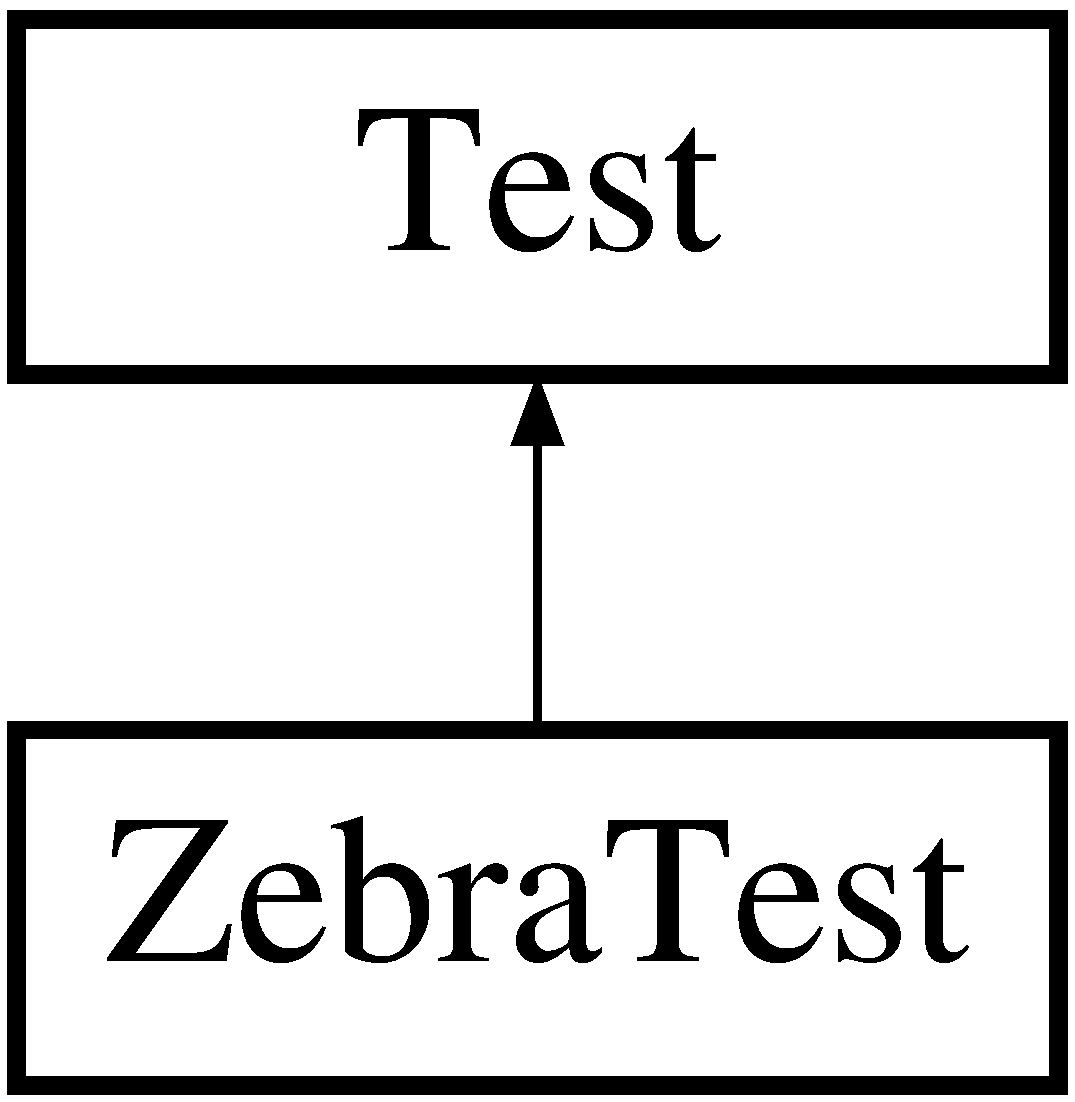
\includegraphics[height=2.000000cm]{class_zebra_test}
\end{center}
\end{figure}


The documentation for this class was generated from the following file\+:\begin{DoxyCompactItemize}
\item 
main\+\_\+test.\+cpp\end{DoxyCompactItemize}

%--- End generated contents ---

% Index
\backmatter
\newpage
\phantomsection
\clearemptydoublepage
\addcontentsline{toc}{chapter}{Index}
\printindex

\end{document}
